\section{Experiment Details}
\subsection{Benchmark}\label{subapp:benchmark}
\noindent\textbf{NeurIPS 2025 Papers.} We utilize 38 papers accepted at NeurIPS 2025. Specifically, these papers are drawn from benchmarks used in AutoSOTA \citep{li2026autosota}. We provide the full list of papers below.

\begin{table}[h]
\centering
\caption{\textbf{NeurIPS 2025 Papers.} We utilize 38 accepted papers.}\label{tab:neurips}
\resizebox{\textwidth}{!}{
\begin{tabular}{l}
\toprule
\textbf{Title}\\
\midrule
SAVVY: Spatial Awareness via Audio-Visual LLMs through Seeing and Hearing \citep{chen2025savvy}\\
PhySense: Sensor Placement Optimization for Accurate Physics Sensing \citep{ma2025physense}\\
Hogwild! Inference: Parallel LLM Generation via Concurrent Attention \citep{rodionov2025hogwild}\\
On the Integration of Spatial-Temporal Knowledge: A Lightweight Approach to Atmospheric Time Series Forecasting \citep{fu2025on}\\
CausalPFN: Amortized Causal Effect Estimation via In-Context Learning \citep{balazadeh2025causalpfn}\\
Accelerating Feature Conformal Prediction via Taylor Approximation \citep{tang2025accelerating}\\
Multi-Task Vehicle Routing Solver via Mixture of Specialized Experts under State-Decomposable MDP \citep{pan2025multitask}\\
Stochastic Forward-Forward Learning through Representational Dimensionality Compression \citep{zhu2025stochastic}\\
Tree Ensemble Explainability through the Hoeffding Functional Decomposition and TreeHFD Algorithm \citep{benard2025tree}\\
X-Mahalanobis: Transformer Feature Mixing for Reliable OOD Detection \citep{wei2025xmahalanobis}\\
Iterative Missing Data Imputation with Model Form Adaptation and Non-Missing Feature Supervision \citep{wang2025iterative}\\
Neural MJD: Neural Non-Stationary Merton Jump Diffusion for Time Series Prediction \citep{gao2025neural}\\
Mind-the-Glitch: Visual Correspondence for Detecting Inconsistencies in Subject-Driven Generation \citep{eldesokey2025mindtheglitch}\\
Tree-Sliced Entropy Partial Transport \citep{tran2025treesliced}\\
Balanced Active Inference \citep{chen2025balanced}\\
Wasserstein Transfer Learning \citep{zhang2025wasserstein}\\
Fast Non-Log-Concave Sampling under Nonconvex Equality and Inequality Constraints with Landing \citep{jeon2025fast}\\
Efficient Training-Free Online Routing for High-Volume Multi-LLM Serving \citep{wu2025efficient}\\
Multi-Class Support Vector Machine with Differential Privacy \citep{park2025multiclass}\\
FedWMSAM: Fast and Flat Federated Learning via Weighted Momentum and Sharpness-Aware Minimization \citep{li2025fedwmsam}\\
MDReID: Modality-Decoupled Learning for Any-to-Any Multi-Modal Object Re-Identification \citep{feng2025mdreid}\\
Aligning Evaluation with Clinical Priorities: Calibration, Label Shift, and Error Costs \citep{flores2025aligning}\\
Measure-Theoretic Anti-Causal Representation Learning \citep{behnam2025measuretheoretic}\\
STaRFormer: Semi-Supervised Task-Informed Representation Learning via Dynamic Attention-Based Regional Masking for Sequential Data \citep{forstenhausler2025starformer}\\
Improving Time Series Forecasting via Instance-aware Post-hoc Revision \citep{liu2025improving}\\
Tropical Attention: Neural Algorithmic Reasoning for Combinatorial Algorithms \citep{hashemi2025tropical}\\
AANet: Virtual Screening under Structural Uncertainty via Alignment and Aggregation \citep{zhu2025aanet}\\
NeuralSurv: Deep Survival Analysis with Bayesian Uncertainty Quantification \citep{monod2025neuralsurv}\\
TS-RAG: Retrieval-Augmented Generation based Time Series Foundation Models are Stronger Zero-Shot Forecaster \citep{ning2025tsrag}\\
SEMPO: Lightweight Foundation Models for Time Series Forecasting \citep{he2025sempo}\\
IA-GGAD: Zero-shot Generalist Graph Anomaly Detection via Invariant and Affinity Learning \citep{zhang2025iaggad}\\
Mean Flows for One-step Generative Modeling \citep{geng2025mean}\\
ProxySPEX: Inference-Efficient Interpretability via Sparse Feature Interactions in LLMs \citep{butler2025proxyspex}\\
Not All Data are Good Labels: On the Self-supervised Labeling for Time Series Forecasting \citep{yang2025not}\\
Towards Accurate Time Series Forecasting via Implicit Decoding \citep{li2025towards}\\
Least squares variational inference \citep{fay2025least}\\
CSBrain: A Cross-scale Spatiotemporal Brain Foundation Model for EEG Decoding \citep{zhou2025csbrain}\\
Hierarchical Shortest-Path Graph Kernel Network \citep{wang2025hierarchical}\\
\bottomrule
\end{tabular}}
\end{table}

\noindent\textbf{ICLR 2026 Papers.} We utilize 5 papers accepted at ICLR 2026. Specifically, these papers are drawn from benchmakrs used in AutoSOTA \citep{li2026autosota}. We provide the full list of papers below.

\begin{table}[h]
\centering
\caption{\textbf{ICLR 2026 Papers.} We utilize 5 accepted papers.}\label{tab:iclr}
\resizebox{\textwidth}{!}{
\begin{tabular}{l}
\toprule
\textbf{Title}\\
\midrule
Temporal Sparse Autoencoders: Leveraging the Sequential Nature of Language for Interpretability \citep{bhalla2026temporal}\\
Pinet: Optimizing hard-constrained neural networks with orthogonal projection layers \citep{grontas2026pinet}\\
Discount Model Search for Quality Diversity Optimization in High-Dimensional Measure Spaces \citep{tjanaka2026discount}\\
Reasoning as Representation: Rethinking Visual Reinforcement Learning in Image Quality Assessment \citep{zhao2026reasoning}\\
Decentralized Attention Fails Centralized Signals: Rethinking Transformers for Medical Time Series \citep{yu2026decentralized}\\
\bottomrule
\end{tabular}}
\end{table}

\noindent\textbf{ICML 2026 Spotlight Papers.} We utilize 64 papers accepted as spotlight presentations at ICML 2026. Specifically, these 64 papers were selected from among all spotlight papers by strictly adhering to AutoSOTA's filtering process (e.g., verifying reproducibility).
We provide the full list of papers below.

\begin{table}[!ht]
\centering
\caption{\textbf{ICML 2026 Spotlight Papers.} We utilize 64 papers accepted as spotlight presentations.}\label{tab:icml}
\resizebox{\textwidth}{!}{
\begin{tabular}{l}
\toprule
\textbf{Title}\\
\midrule
A Fully First-Order Layer for Differentiable Optimization \citep{zhao2025fully}\\
Mixture of Concept Bottleneck Experts \citep{santis2026mixture}\\
Mechanistic Data Attribution: Tracing the Training Origins of Interpretable LLM Units \citep{chen2026mechanistic}\\
Loss-Aware Distributionally Robust Optimization via Trainable Optimal Transport Ambiguity Sets \citep{ohnemus2026lossaware}\\
SceneSmith: Agentic Generation of Simulation-Ready Indoor Scenes \citep{pfaff2026scenesmith}\\
Reward Redistribution for CVaR MDPs using a Bellman Operator on L-infinity \citep{muni2026reward}\\
Incremental BPE Tokenization \citep{jiang2026incremental}\\
Towards Optimal Robustness in Learning-Augmented Paging \citep{chen2026towards}\\
Many Experiments, Few Repetitions, Unpaired Data, and Sparse Effects: Is Causal Inference Possible? \citep{schur2026many}\\
AI Engram: In Search of Memory Traces in Artificial Intelligence \citep{kwon2026ai}\\
OC-space: a Unifying Perspective on Verification of Tree Ensembles \citep{martens2026ocspace}\\
RED-HDP-HMM: Observation-Dependent Durations for Bayesian Nonparametric Sequential Models \citep{supinski2026redhdphmm}\\
Optimal Decision-Making Based on Prediction Sets \citep{wang2026optimal}\\
Protein Fold Classification at Scale: Benchmarking and Pretraining \citep{chen2026protein}\\
Geometry-Aware Decoding with Wasserstein-Regularized Truncation and Mass Penalties for Large Language Models \citep{davoodi2026geometryaware}\\
Conformal Policy Control \citep{prinster2026conformal}\\
Towards Long-Horizon Interpretability: Efficient and Faithful Multi-Token Attribution for Reasoning LLMs \citep{pan2026towards}\\
Rare Event Analysis of Large Language Models \citep{dorman2026rare}\\
When to Trust the Cheap Check: Weak and Strong Verification for Reasoning \citep{kiyani2026when}\\
Harnessing Non-Adversarial Robustness in Large Language Models \citep{zhou2026harnessing}\\
DAVE: Distribution-Aware Attribution via ViT Gradient Decomposition \citep{wrobel2026dave}\\
Balancing Understanding and Generation in Discrete Diffusion Models \citep{liu2026balancing}\\
Exact Functional ANOVA Decomposition for Categorical Inputs Models \citep{ferrere2026exact}\\
Asymmetric Perturbation in Solving Bilinear Saddle-Point Optimization \citep{abe2026asymmetric}\\
Control Consistency Losses for Diffusion Bridges \citep{howard2026control}\\
Deep Flow Networks \citep{candogan2026deep}\\
A Factorized Low-Rank RNN Framework for Uncovering Independent Neural Latent Dynamics and Connectivity \citep{li2026a}\\
FlashSinkhorn: IO-Aware Entropic Optimal Transport on GPU \citep{ye2026flashsinkhorn}\\
Near-Optimal Private Linear Regression via Iterative Hessian Mixing \citep{lev2026nearoptimal}\\
Rethinking LLM Ensembling from the Perspective of Mixture Models \citep{fu2026rethinking}\\
Controlled LLM Training on Spectral Sphere \citep{xie2026controlled}\\
TG-RAG: A Retrieval-Augmented Framework for Reasoning Guidance in Specialized Domains \citep{su2026tgrag}\\
Time series saliency maps: Explaining models across multiple domains \citep{kechris2026time}\\
Online Conformal Prediction via Universal Portfolio Algorithms \citep{liu2026online}\\
Characterizing, Evaluating, and Optimizing Complex Reasoning \citep{zhang2026characterizing}\\
The Value of Variance: Mitigating Debate Collapse in Multi-Agent Systems via Uncertainty-Driven Policy Optimization \citep{tang2026the}\\
EEmo-Logic: A Unified Dataset and Multi-Stage Framework for Comprehensive Image-Evoked Emotion Assessment \citep{gao2026eemologic}\\
From Text to Forecasts: Bridging Modality Gap with Temporal Evolution Semantic Space \citep{li2026from}\\
3ViewSense: Spatial and Mental Perspective Reasoning from Orthographic Views in Vision-Language Models \citep{zhan2026viewsense}\\
Efficient numeracy in language models through single-token number embeddings \citep{kreitner2026efficient}\\
EgoTactile: Learning Grasp Pressure for Everyday Objects from Egocentric Video \citep{zeng2026egotactile}\\
Learning to Discover at Test Time \citep{yuksekgonul2026learning}\\
OPUS: Towards Efficient and Principled Data Selection in Large Language Model Pre-training in Every Iteration \citep{wang2026opus}\\
GEM: Geometric Erasure by Contrastive Velocity Matching in Rectified Flows \citep{grebe2026gem}\\
Steer Like the LLM: Activation Steering that Mimics Prompting \citep{heyman2026steer}\\
The Flexibility Trap: Rethinking the Value of Arbitrary Order in Diffusion Language Models \citep{ni2026the}\\
Scalable Option Learning in High-Throughput Environments \citep{henaff2026scalable}\\
On the Difficulty of Learning a Meta-network for Training Data Selection \citep{du2026on}\\
Reinforced Sequential Monte Carlo for Amortised Sampling \citep{choi2026reinforced}\\
Language Model Circuits Are Sparse in the Neuron Basis \citep{arora2026language}\\
Unifying and Optimizing Data Values for Selection via Sequential Decision-Making \citep{chi2026unifying}\\
Neural Thickets: Diverse Task Experts Are Dense Around Pretrained Weights \citep{gan2026neural}\\
Initialization is Half the Battle: Generating Diverse Images from a Guidance Potential Posterior \citep{li2026initialization}\\
FlashOptim: Optimizers for Memory-Efficient Training \citep{ortiz2026flashoptim}\\
Bulk-Calibrated Credal Ambiguity Sets: Fast, Tractable Decision Making under Out-of-Sample Contamination \citep{chen2026bulkcalibrated}\\
Maximum Likelihood Reinforcement Learning \citep{tajwar2026maximum}\\
Learning Randomized Reductions \citep{erata2024learning}\\
SVL: Empowering Spiking Neural Networks for Efficient 3D Open-World Understanding \citep{qiu2026svl}\\
TabSwift: An Efficient Tabular Foundation Model with Row-Wise Attention \citep{liu2026tabswift}\\
Thinking in Flow: A Dissipative Stabilization Operator for Robust Autoregressive Reasoning \citep{huang2026thinking}\\
VALUEFLOW: Toward Pluralistic and Steerable Value-based Alignment in Large Language Models \citep{kim2026valueflow}\\
Mixtures Closest To A Given Measure: A Semidefinite Programming Approach \citep{durasinovic2026mixtures}\\
Welfare-Optimal Classification with Accuracy Auctions \citep{sadi2026welfareoptimal}\\
Efficient Parallel Samplers for Recurrent-Depth Models and Their Connection to Diffusion Language Models \citep{geiping2026efficient}\\
\bottomrule
\end{tabular}}
\end{table}

\newpage
\subsection{Configuration}\label{subapp:config}
Unless otherwise specified, we employ Gemini 3.6 Flash for all agents, except for the Idea Experiment Coding Agent, the Ablation Study Agent, the Rebuttal Agent, and the Draft Enhancer, which use Claude Code with Opus 4.8. To evaluate novelty, \sname~retrieves two reference papers via Google Search. We extract limitations for a maximum of 16 rounds. In each idea experimentation round, we evaluate two candidates: one selected from the seed ideas and the other an evolved idea. We run this experimentation loop for up to four rounds, terminating early once four successful ideas are obtained. If the Idea Critic Agent flags an idea for engineering refinement, we apply engineering techniques for at most two rounds. Similarly, when the Ablation Critic Agent recommends refinement based on ablation results, we refine the idea at most once. Finally, the peer-review simulation runs for at most two rounds and terminates early if the ScholarPeer review score reaches 8, with review-based refinement conducted at most once. We use the ICLR 2025 format for drafting, following the PaperOrchestra.





% ---------------------------------------------------------------------------
% Detailed comparison: ScientistTwo vs. AutoSOTA on the 5 ICLR-2026 papers.
% Requires: booktabs.
% ---------------------------------------------------------------------------

\section{Detailed Comparison with AutoSOTA}
\label{sec:autosota}

\begin{table}[h]
\centering
\small
\setlength{\tabcolsep}{5pt}
\renewcommand{\arraystretch}{1.1}
\caption{\textbf{Aggregate differences} over the five papers. The two systems apply different
acceptance rules: AutoSOTA halts as soon as a pre-registered numerical target is cleared (e.g. after a
single iteration on DMSQD~\citep{tjanaka2026discount}), whereas ScientistTwo has no target metric
and additionally requires the gain to be attributable to the proposed mechanism in ablation.}
\label{tab:autosota-quant}
\begin{tabular}{@{}lcc@{}}
\toprule
& \textbf{AutoSOTA} & \textbf{ScientistTwo} \\
\midrule
Papers with a reported gain             & 5\,/\,5 & 4\,/\,5 \\
Typical change                     & config & new modules \\
New algorithmic component               & 0\,/\,5 & 4\,/\,4 \\
Modifies the evaluation protocol        & 1\,/\,5 & forbidden (audit) \\
Evaluated on the full benchmark         & 0\,/\,5 & 4\,/\,4 \\
Component-level attribution             & none & 5--6 ablations per paper \\
Produces a reviewable paper             & no & yes   \\
\bottomrule
\end{tabular}
\end{table}

\noindent We run ScientistTwo on the same five ICLR~2026 submissions (Table~\ref{tab:iclr}) that
AutoSOTA reports. The two systems are built for different objectives. AutoSOTA is an
end-to-end, metric-driven optimizer: starting from a raw paper, it locates the repository,
reconstructs a runnable baseline, and distills the paper's headline result into a single
numerical target, then proposes and benchmarks edits until that target is cleared. It does
construct a multi-dimensional rubric, but the optimization loop is driven by that one
result-match number. In contrast, ScientistTwo operates without predefined numerical targets—it must independently diagnose research limitations, formulate a novel methodology, implement and ablate the proposed approach, and produce a complete scientific manuscript.

Table~\ref{tab:autosota-quant} summarizes the quantitative differences, while Table~\ref{tab:autosota-qual} provides a qualitative comparison of the modifications introduced by each system. Because each system measures against its own reproduced baseline on different hardware, the two $\Delta$ columns are not a head-to-head on a common metric; they characterize the \emph{nature} and \emph{scope} of each change.


\textbf{What gets optimized.}
For these ICLR2026 papers, every AutoSOTA improvement is a configuration change inside an existing code path: solver
iterations and float precision~\citep{grontas2026pinet}, emitter count~\citep{tjanaka2026discount},
model width and optimizer~\citep{yu2026decentralized}, a threshold in the evaluation
harness~\citep{bhalla2026temporal}, and the mixing weights of three already-implemented pooling
paths~\citep{zhao2026reasoning}. No new algorithmic component appears in any of the five, and the
median change is under ten lines. ScientistTwo's accepted solutions instead introduce
transferable mechanisms: a nullspace re-parameterization that makes the equality constraints of
Pinet~\citep{grontas2026pinet} exact by construction, a sheaf-Laplacian/Koopman training
objective for T-SAE~\citep{bhalla2026temporal}, adversarial content--quality disentanglement
with region-level quality segmentation for RALI~\citep{zhao2026reasoning}, and a dimension-adaptive
smoothness penalty on the discount model for DMSQD~\citep{tjanaka2026discount}.

\noindent\textbf{What counts as success.}
The two systems disagree about what a success \emph{is}, and this drives
most of the divergence. On TeCh~\citep{yu2026decentralized}, AutoSOTA reports $+4.45\%$ accuracy
from widening the backbone and adding label smoothing. ScientistTwo found the same lever: its
\textsc{DMC-TeCh} variant beat the baseline on 5 of 6 metrics, but the ablation critic rejected
it because ``the gains were primarily driven by general training controls (EMA and label
smoothing) rather than the multi-core architectural innovation itself,'' so it was not accepted
as a contribution. A metric-movement criterion and an attribution criterion score generic
capacity tuning in opposite directions.

\noindent\textbf{Robustness and scope.}
Optimizing a single registered number exposes two classic failure modes. \emph{Unmeasured
trade-offs}: on Pinet~\citep{grontas2026pinet} the dominant edit removes exactly the solver work
that controls constraint violation, which is not in the registered metric, so the $-16.7\%$
latency is reported with no feasibility number. \emph{Optimizing the evaluator}: on
T-SAE~\citep{bhalla2026temporal} the winning change alters how activations are displayed to the
LLM judge, leaving the SAE untouched, and AutoSOTA's own re-evaluation returns $0.7557$, below the
$0.7586$ baseline. AutoSOTA does declare red lines against exactly these failures (R1--R2 forbid
altering the evaluation script or metric parameters, and R4 constrains cross-metric trade-offs), but they fail empirically on both cases here. ScientistTwo instead blocks both structurally, via a
reproduction re-run (I1), a protocol-immutability audit (I2), and a method--code alignment audit
(I4) rather than a prompt-level list of prohibitions, and evaluates on the paper's full benchmark
grid rather than the single registered split.

\noindent\textbf{Complementarity.}
The two systems are not strictly ordered, and DMSQD~\citep{tjanaka2026discount} shows why: both
improve QD score, but along orthogonal axes. AutoSOTA raises the emitter count $15\!\to\!20$,
buying its $+33\%$ evaluations per iteration---a pure compute-scaling knob that our idea generator
deliberately does not propose. ScientistTwo instead leaves the compute budget fixed and improves
the discount model itself, adding a dimension-adaptive contact-form smoothness penalty
(\textsc{LC-FTT}) that lifts DMS in high-dimensional measure spaces ($+422$ QD $/\,{+}1.16$pp
coverage averaged, reproduced bit-exact). The two changes touch disjoint parts of the pipeline and
compose. We therefore see the systems as complementary
stages: ScientistTwo produces a method, and a tuner such as AutoSOTA can then optimize its
deployment constants---and where a headline metric is near-monotone in compute, a short tuning loop
is the cheaper tool for that last mile.


% ---------------------------------------------------------------------------
\newpage
\begin{table}[h!]
\centering
\footnotesize
\setlength{\tabcolsep}{3pt}
\renewcommand{\arraystretch}{1.1}
\caption{\textbf{Paper-by-paper comparison} on the five submissions of Table~\ref{tab:iclr}.
$\Delta$ is self-reported by each system against its own reproduced baseline; the two columns
optimize different metrics in three of five cases and are not a head-to-head.}
\label{tab:autosota-qual}
\begin{tabular}{@{}p{0.085\textwidth}p{0.25\textwidth}p{0.30\textwidth}p{0.27\textwidth}@{}}
\toprule
\textbf{Paper} & \textbf{AutoSOTA} & \textbf{ScientistTwo} & \textbf{Takeaway} \\
\midrule

Pinet \newline \citep{grontas2026pinet}
& Config tuning, 3 lines change: \texttt{n\_iter\_test} $50\!\to\!10$, \texttt{float64} off,
  \texttt{relu}$\to$\texttt{silu}. Latency $-16.7\%$; feasibility unreported.
& \textsc{ANSE}: amortized Stiefel-nullspace reparameterization (equalities exact by
  construction) $+$ reduced-space Douglas--Rachford $+$ log-barrier feasibility flow. Over the 4
  DC3 sets: RS lower on 3/4 (up to $-69\%$), CV $4\mathrm{e}{-4}\!\to\!2\mathrm{e}{-14}$ on all 4,
  training $3.0\times$ faster.
& AutoSOTA buys latency by deleting the solver work that controls the unmeasured feasibility;
  ScientistTwo makes feasibility structural. Opposite corners of one trade-off. \\
\addlinespace

DMSQD \newline \citep{tjanaka2026discount}
& Config tuning, 1 line change, 1 iteration: emitters $15\!\to\!20$. QD score $+7.3\%$, at $+33\%$
  evaluations per iteration (unreported).
& \textsc{LC-FTT}: a dimension-adaptive contact-form (gradient-norm/Dirichlet-energy) smoothness
  penalty on the DMS discount MLP, disabled in 2D and scaled up with measure dimension. Over the
  full 11-domain grid: beats DMS in high dimensions (up to $+536$ QD $/\,{+}2.08$pp coverage on 10D
  Sphere; $+422$ QD $/\,{+}1.16$pp averaged), $+0.61\%{\pm}0.27$ mean QD over reproduced DMS,
  reproduced bit-exact.
& Same paper, different axes: AutoSOTA scales emitter compute, ScientistTwo improves the discount
  model at fixed budget. The ablation critic stripped LC-FTT's Fisher-Rao/tensor-train/Legendrian
  machinery down to the lone component that carried the gain. Composable, not competing. \\
\addlinespace

TeCh \newline \citep{yu2026decentralized}
& Capacity $+$ regularization: \texttt{d\_model} $256\!\to\!384$, label smoothing, AdamW.
  Accuracy $0.8431\!\to\!0.8806$ ($+4.45\%$).
& \textsc{DMC-TeCh} beat the baseline on 5/6 metrics, but the ablation critic traced the gain to
  EMA $+$ label smoothing rather than to the proposed multi-core mechanism, so it was not
  accepted as a contribution.
& Both systems found the \emph{same} lever and disagree on whether it counts. The gap is
  acceptance policy (metric movement vs.\ attribution), not search capability. \\
\addlinespace

T-SAE \newline \citep{bhalla2026temporal}
& Evaluation-harness tuning, 1 line change: \texttt{act\_threshold\_frac} $0.01\!\to\!0.05$ changes how
  tokens are shown to the LLM judge; the SAE is unchanged. Score $+2.25\%$, but the reported
  re-evaluation is $0.7557 <$ baseline $0.7586$.
& \textsc{Sheaf-SAE}: boundary-gated sheaf Dirichlet energy $+$ causal Koopman operator $+$
  straight-through support projection. Trained from scratch on Pythia-160m and Gemma-2-2b; wins
  Semantics and Context probes on 3/3 suites for both models at matched FVE ($+3.4\%{\pm}0.2$).
& The AutoSOTA gain lives in the evaluator, not the model, and does not survive its own re-run.
  Our I1/I2/I4 audits make this class of edit inadmissible. \\
\addlinespace

RALI \newline \citep{zhao2026reasoning}
& Fusion-weight tuning: tune $\alpha_{\mathrm{cls}}$ over CLS $+$ patch-mean $+$ patch-max, all
  already implemented. PLCC $0.7803\!\to\!0.8012$ ($+2.68\%$) on one split.
& \textsc{DisCoRe-IQA}: LoRA quality adaptation $+$ supervised adversarial content--quality
  disentanglement $+$ region-level quality segmentation. KonIQ-only training, full splits of all
  7 datasets (6 zero-shot): PLCC $+0.006$, SRCC $+0.008$; content probe $0.935\!\to\!0.130$;
  worst-region hit rate $0.899$.
& AutoSOTA's relative $\Delta$ is larger but re-weights existing paths on one split. Ours spans
  seven datasets and adds a capability the paper lacks; an earlier variant was rejected by our
  own critic as statistically inert. \\
\bottomrule
\end{tabular}
\end{table}


\newpage
\section{Qualitative Results}\label{app:qual_results}

In this section, we present qualitative artifacts illustrating the discovery of Procrustes-DS, an out-of-distribution (OOD) detection method designed by \sname{} that outperforms X-Mahalanobis \citep{wei2025xmahalanobis}. We provide representative excerpts generated by \sname~across its research pipeline below, selected from the broader trajectory of hypotheses, explorations, and ablation studies conducted by the framework:
\begin{itemize}
    \item {Limitations of X-Mahalanobis} (pp.~29--30)
    \item {Ideation and Method Proposal} (pp.~31--34)
    \item {Experimental Evaluation Report} (pp.~35--37)
    \item {Ablation Study Report} (pp.~38--40)
    \item {Critic Agent Feedback} (p.~41)
    \item {Reproducibility Audit Report} (p.~42)
    \item {Specification Verification and Method-Code Alignment Audit} (pp.~43--45)
\end{itemize}
For an example of a rebuttal report obtained through a simulated peer-review process, since Procrustes-DS did not undergo this process, the example of TABHARMONY is presented (pp.~46--50).

\section{Case Study: DynaSpec-RAG}\label{app:case_study}
We provide the final draft of DynaSpec-RAG, which is developed by our \sname~(pp.~51--65).

\newpage
\begin{figure}[t!]
    \centering
    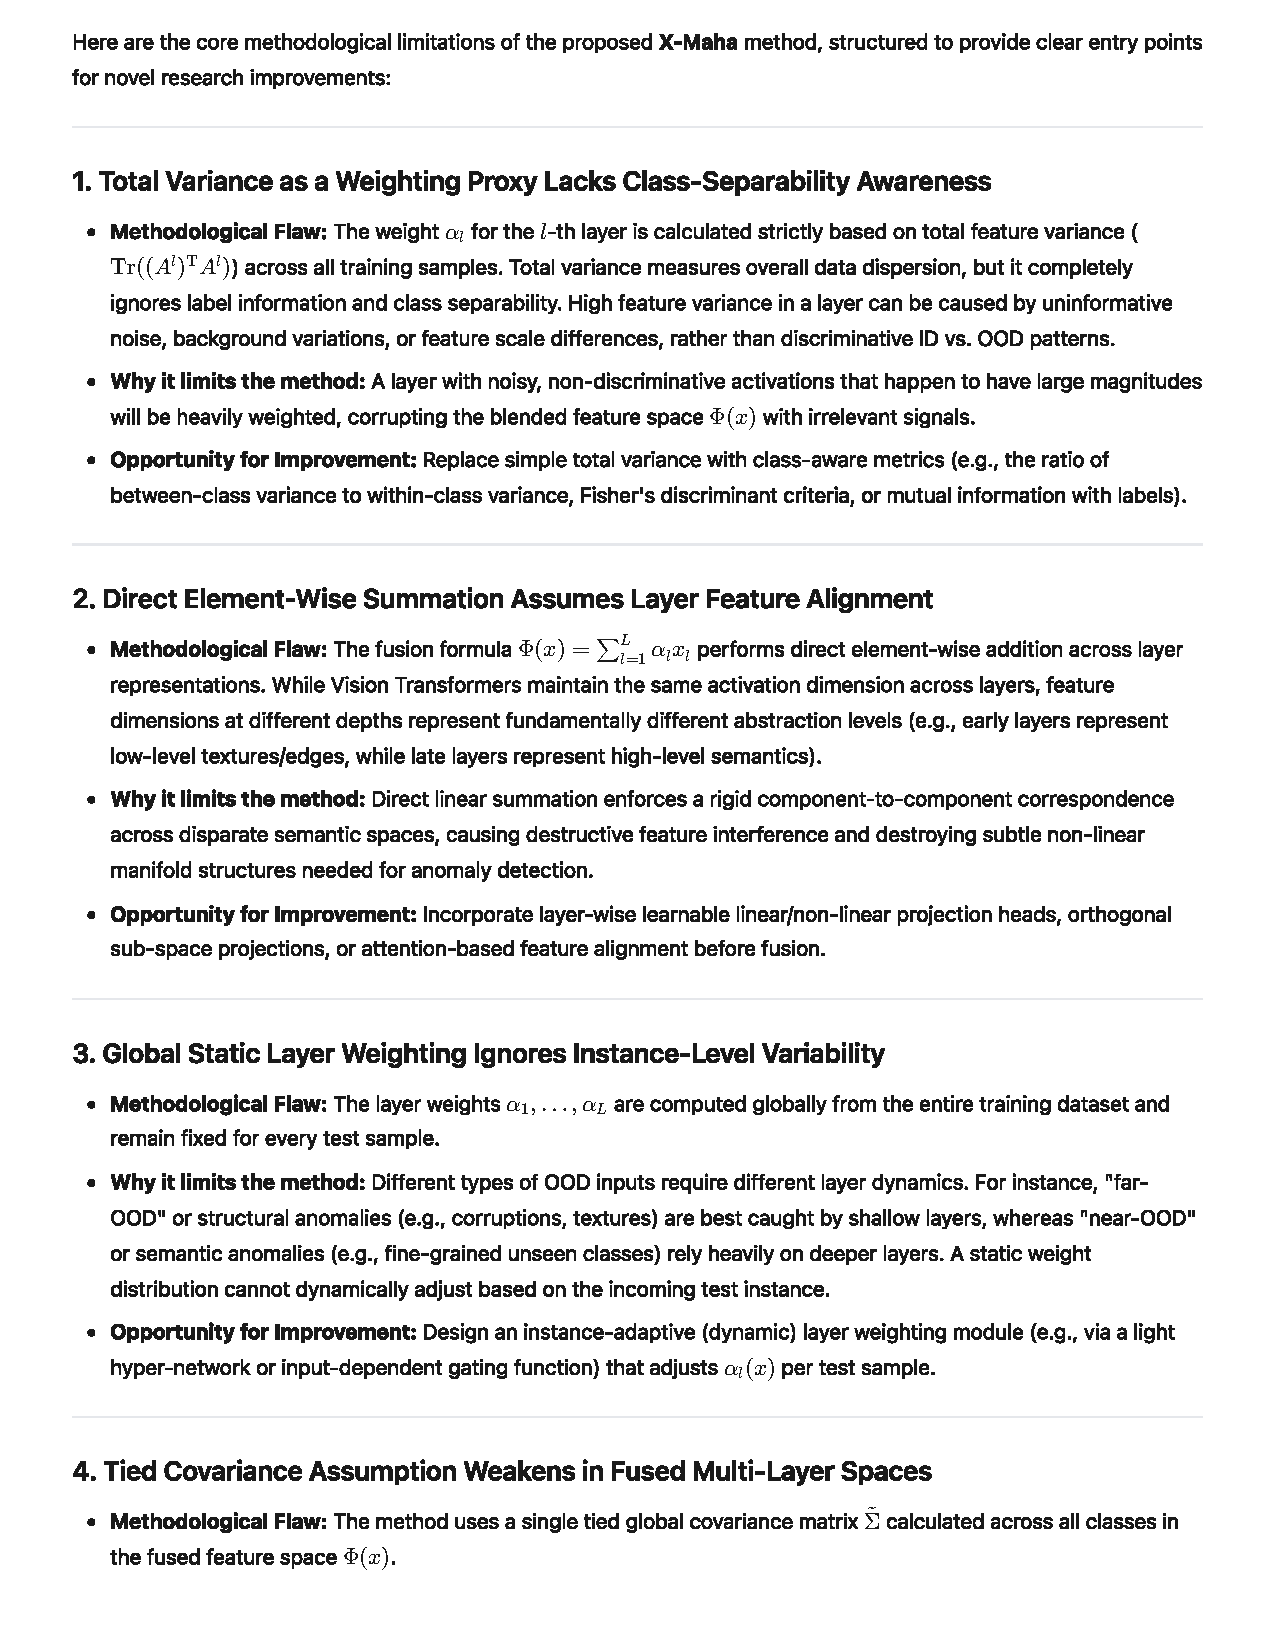
\includegraphics[width=\linewidth]{sections/x_maha_qual/limitation_1.pdf}
\end{figure}

\newpage
\begin{figure}[t!]
    \centering
    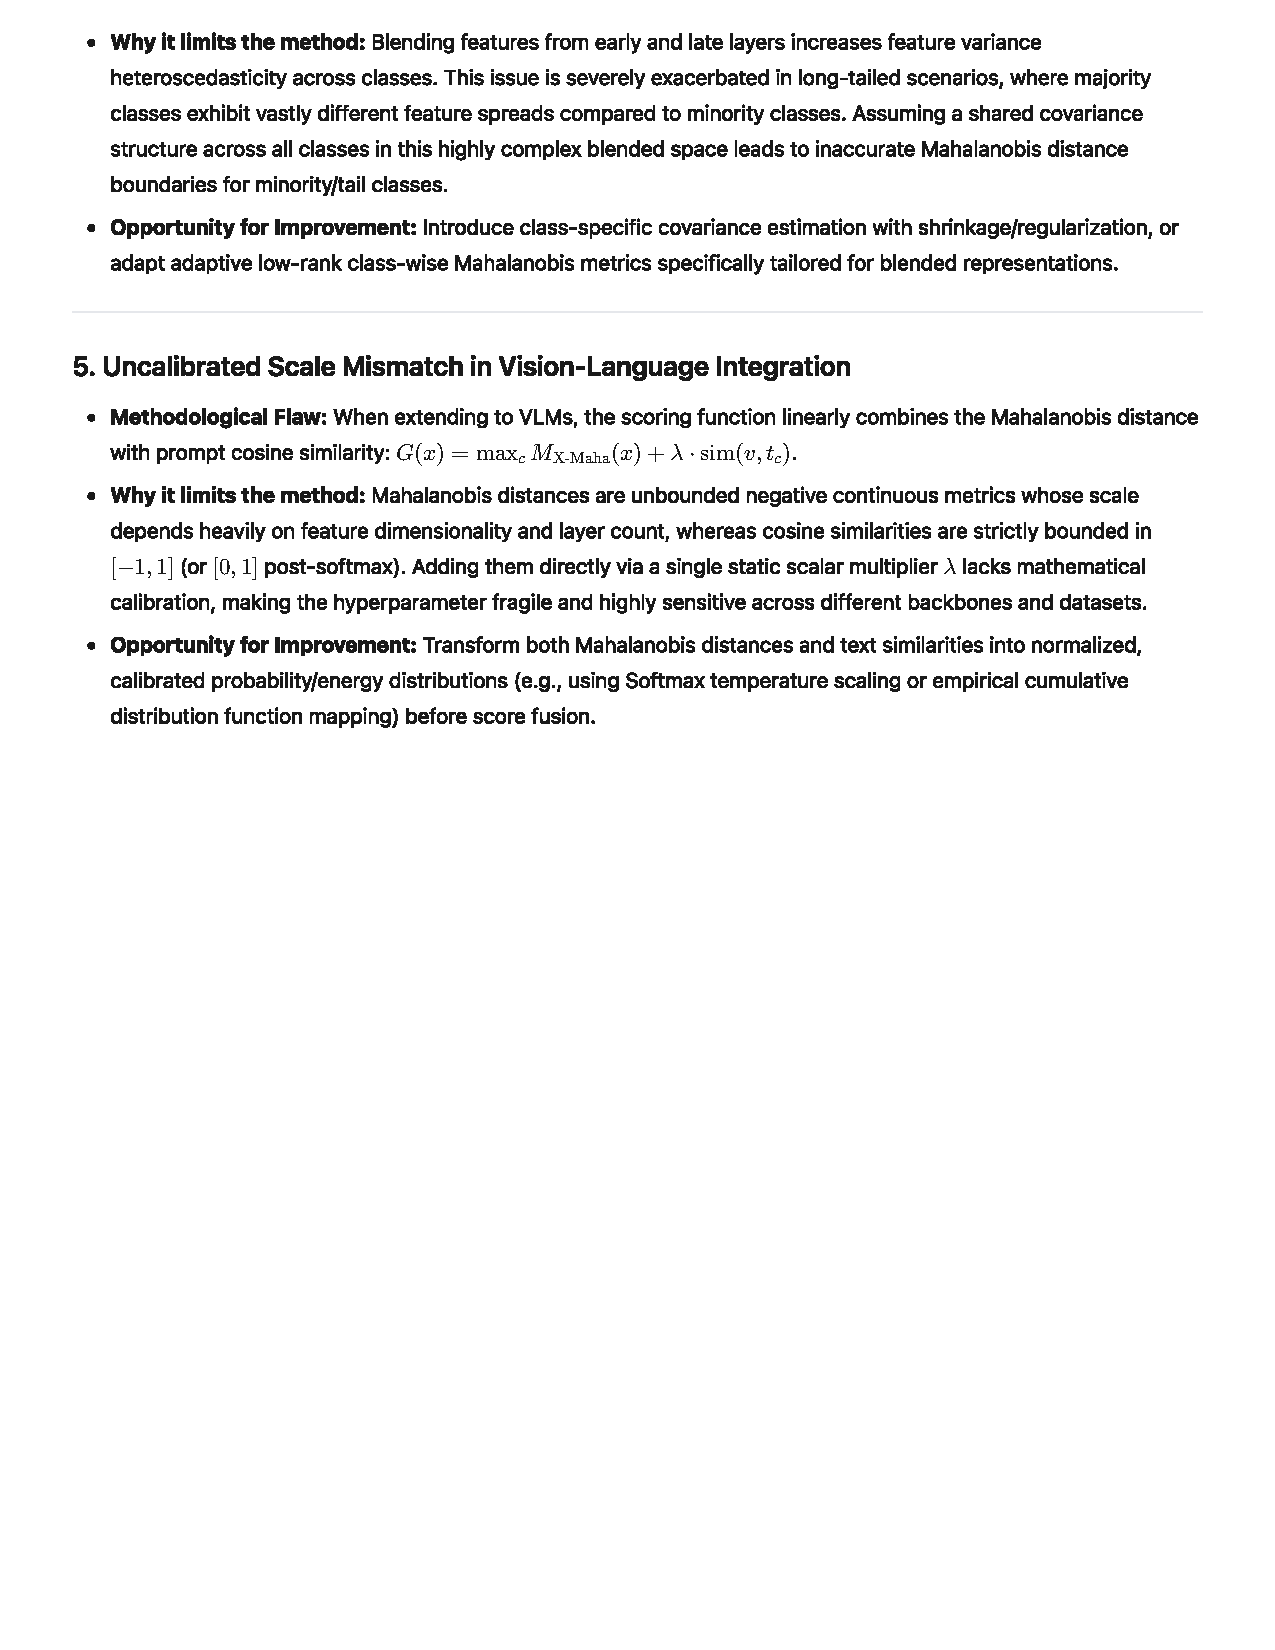
\includegraphics[width=\linewidth]{sections/x_maha_qual/limitation_2.pdf}
\end{figure}

\newpage
\begin{figure}[t!]
    \centering
    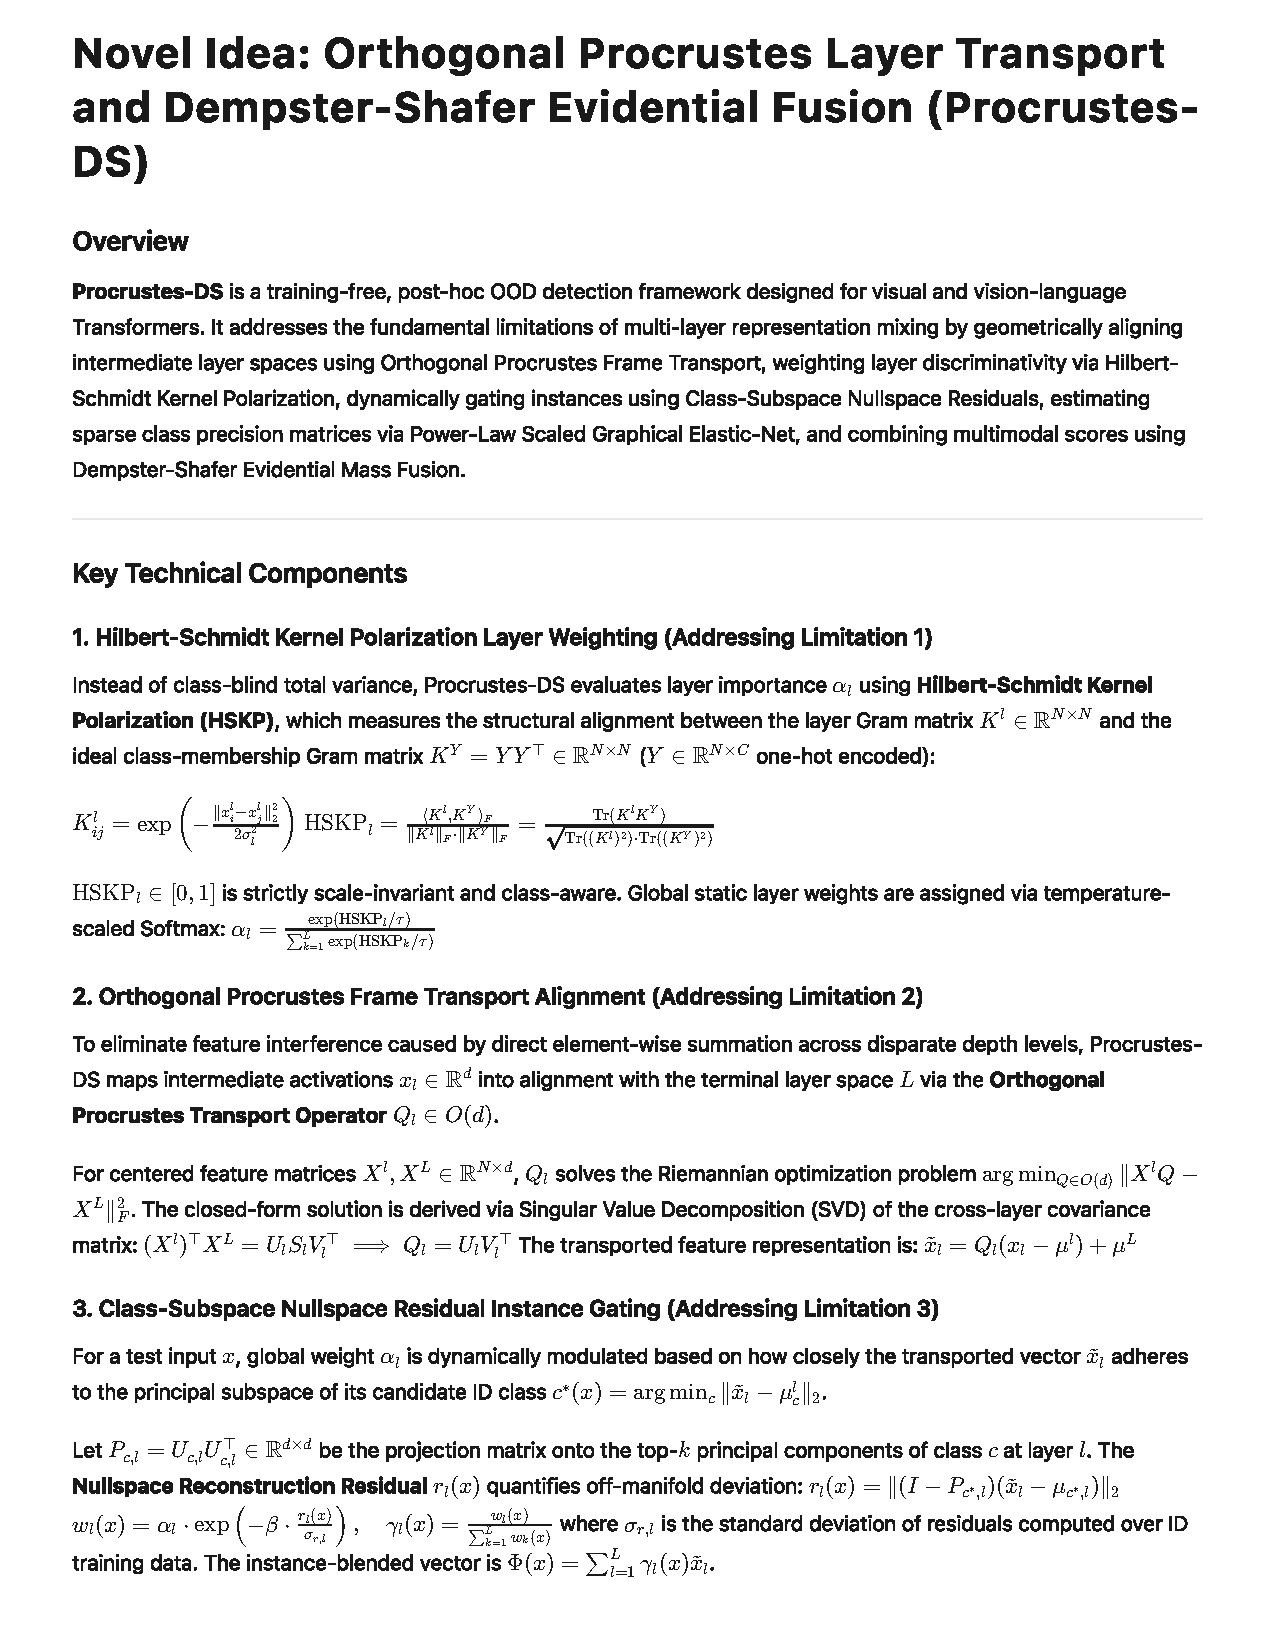
\includegraphics[width=\linewidth]{sections/x_maha_qual/idea_1.pdf}
\end{figure}

\newpage
\begin{figure}[t!]
    \centering
    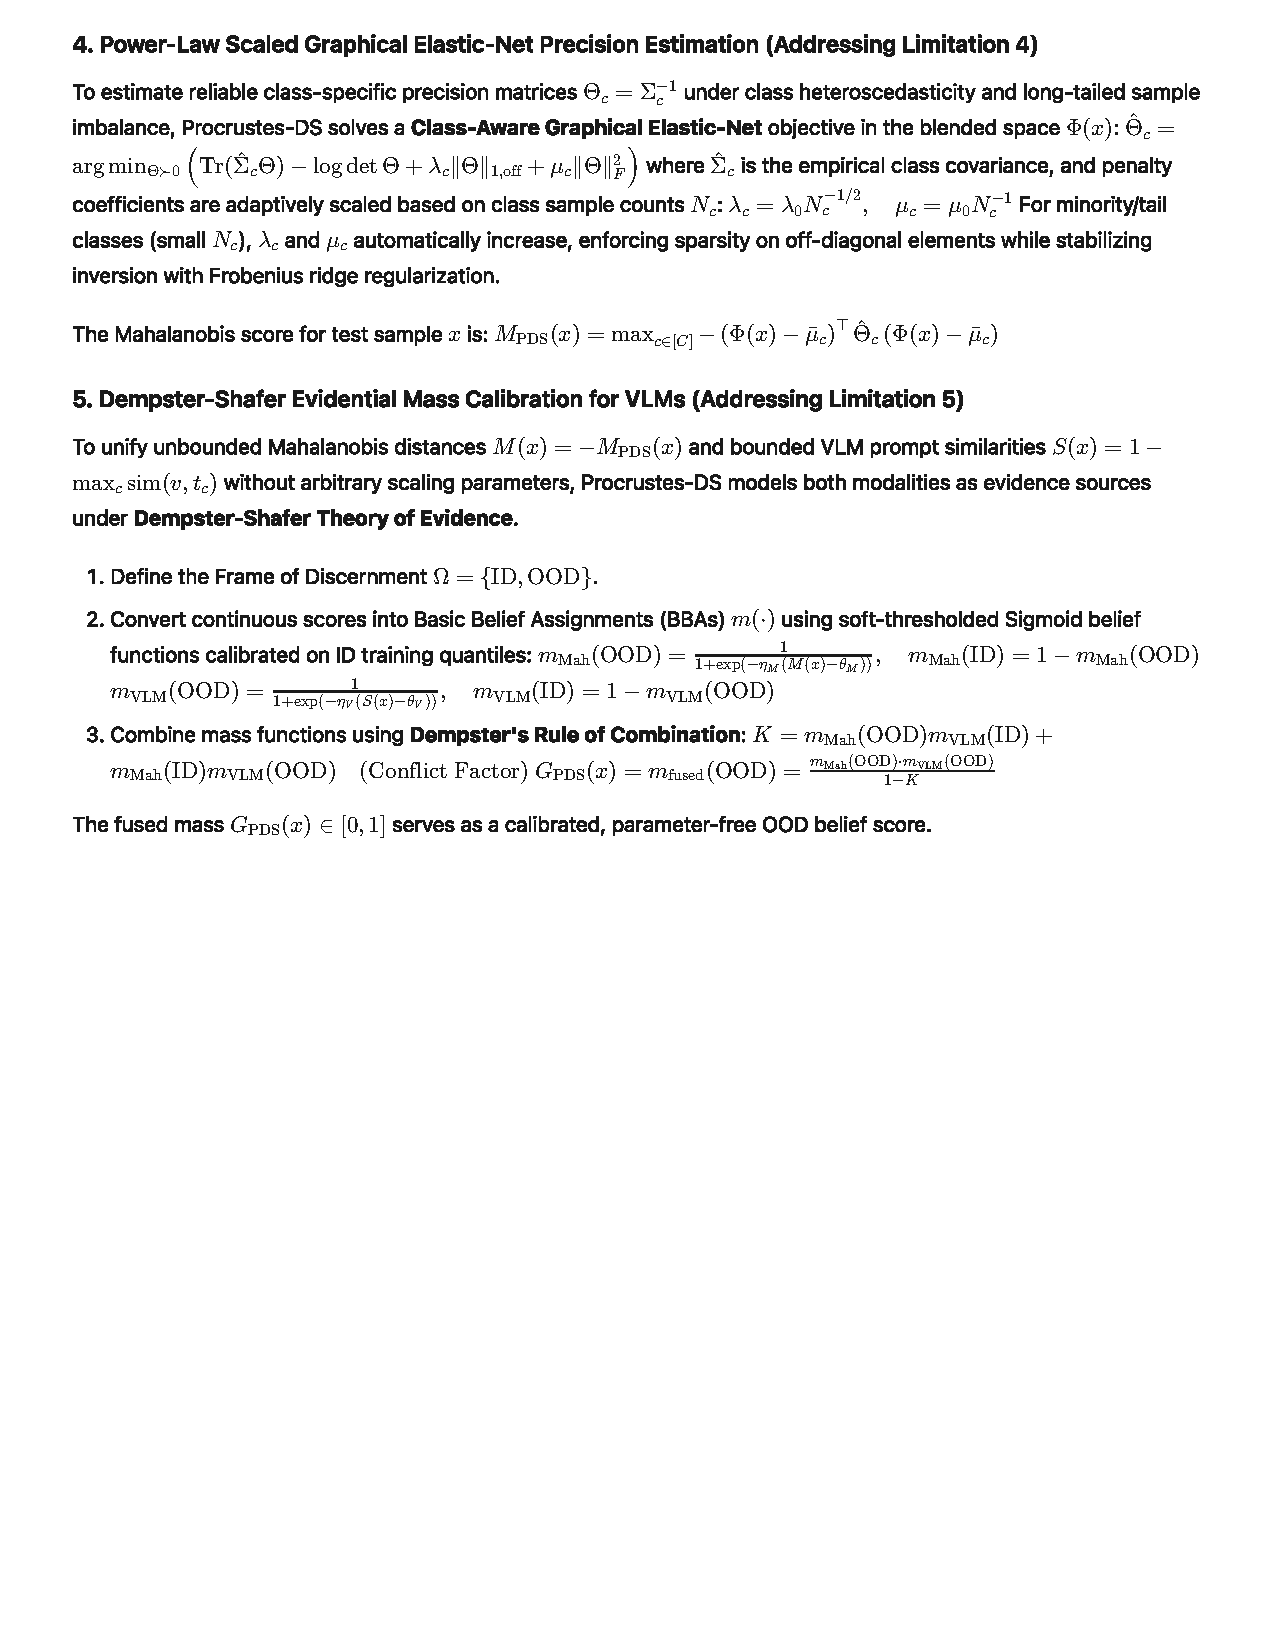
\includegraphics[width=\linewidth]{sections/x_maha_qual/idea_2.pdf}
\end{figure}

\newpage
\begin{figure}[t!]
    \centering
    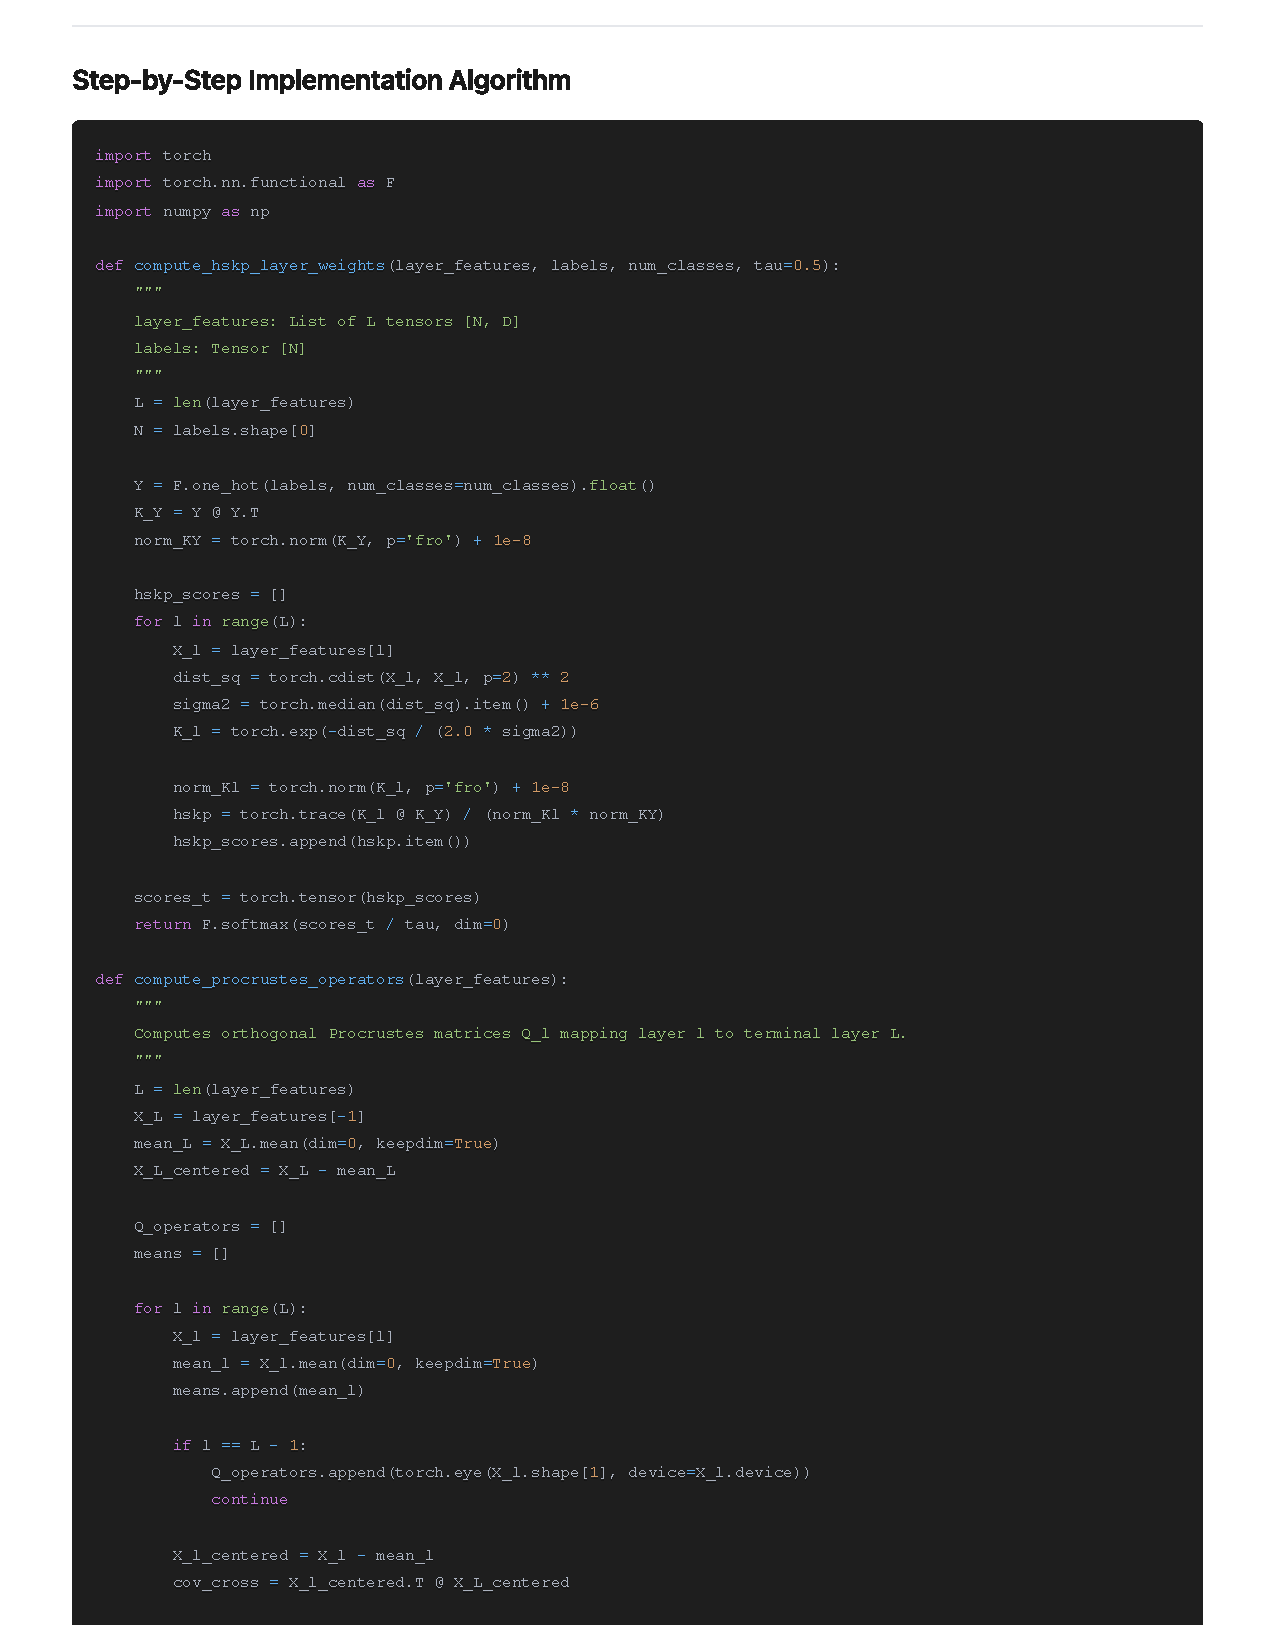
\includegraphics[width=\linewidth]{sections/x_maha_qual/idea_3.pdf}
\end{figure}

\newpage
\begin{figure}[t!]
    \centering
    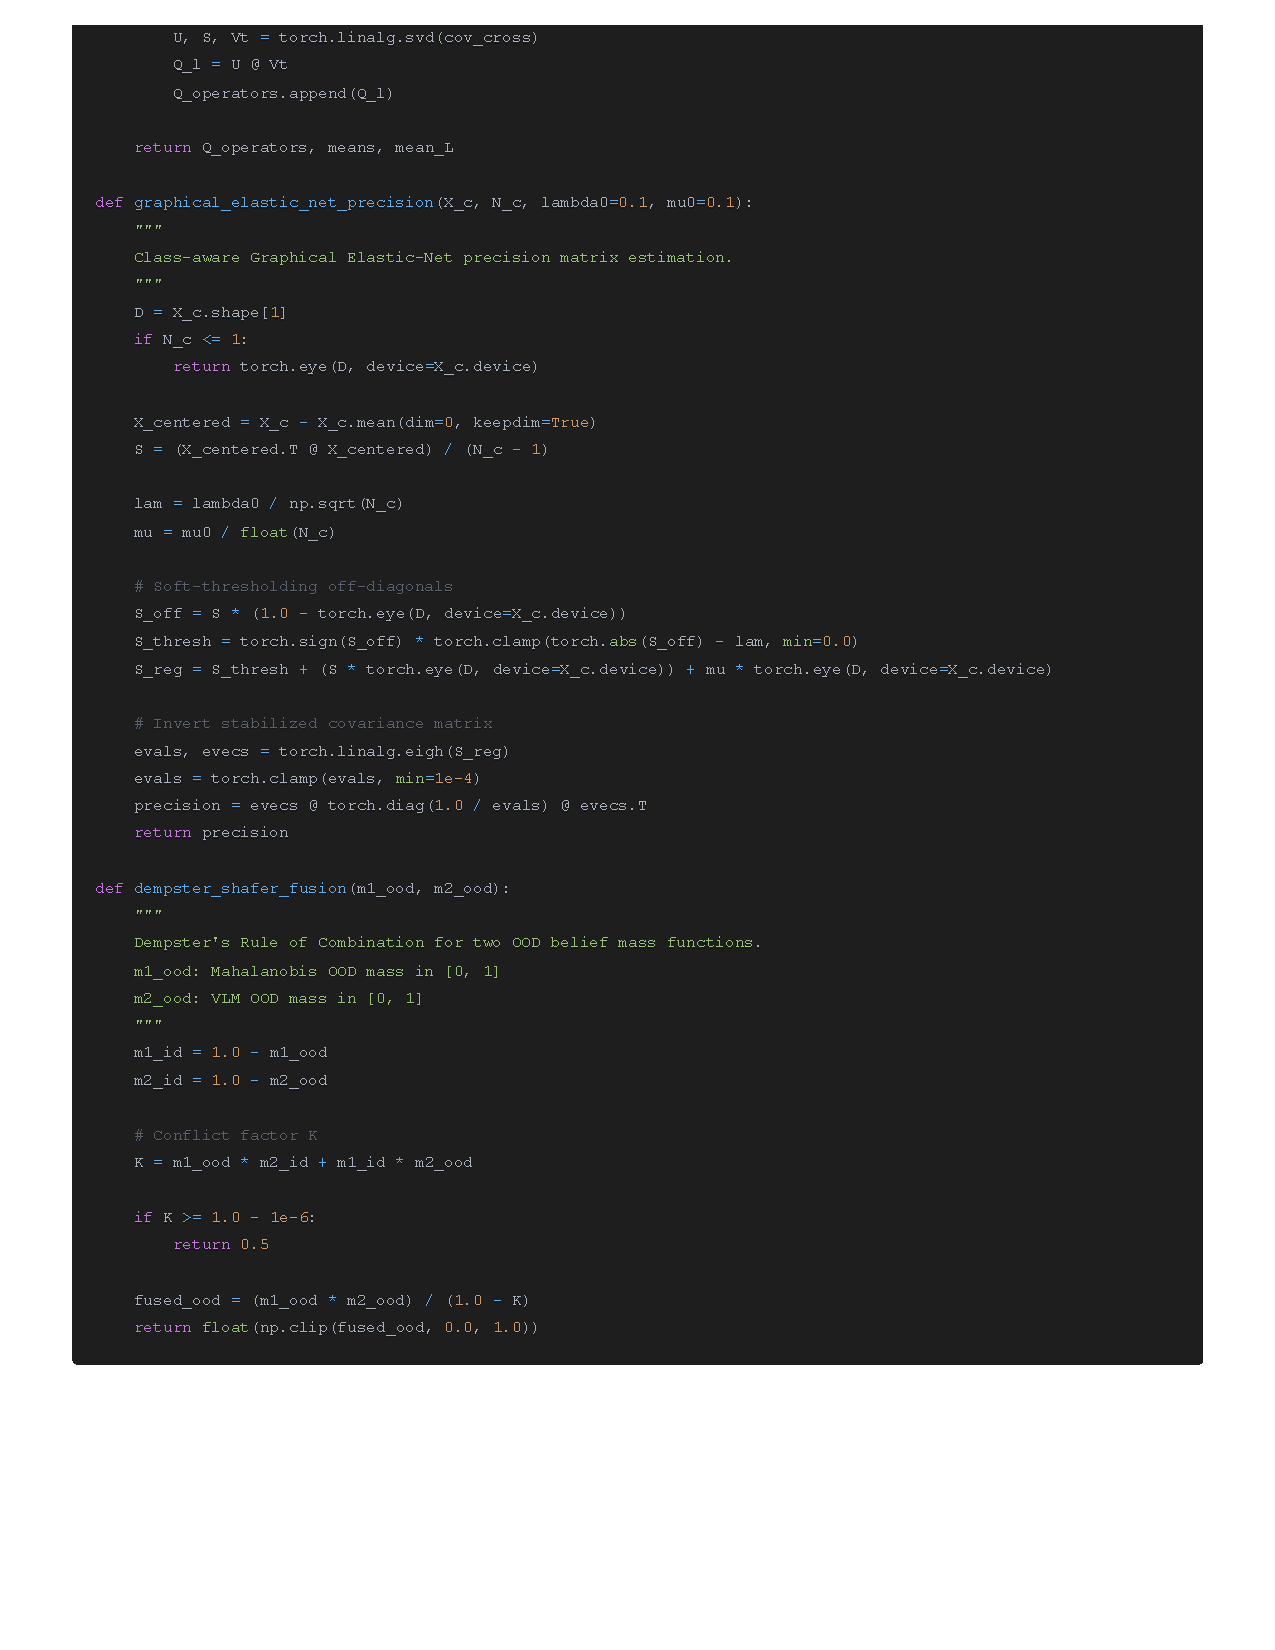
\includegraphics[width=\linewidth]{sections/x_maha_qual/idea_4.pdf}
\end{figure}

\newpage
\begin{figure}[t!]
    \centering
    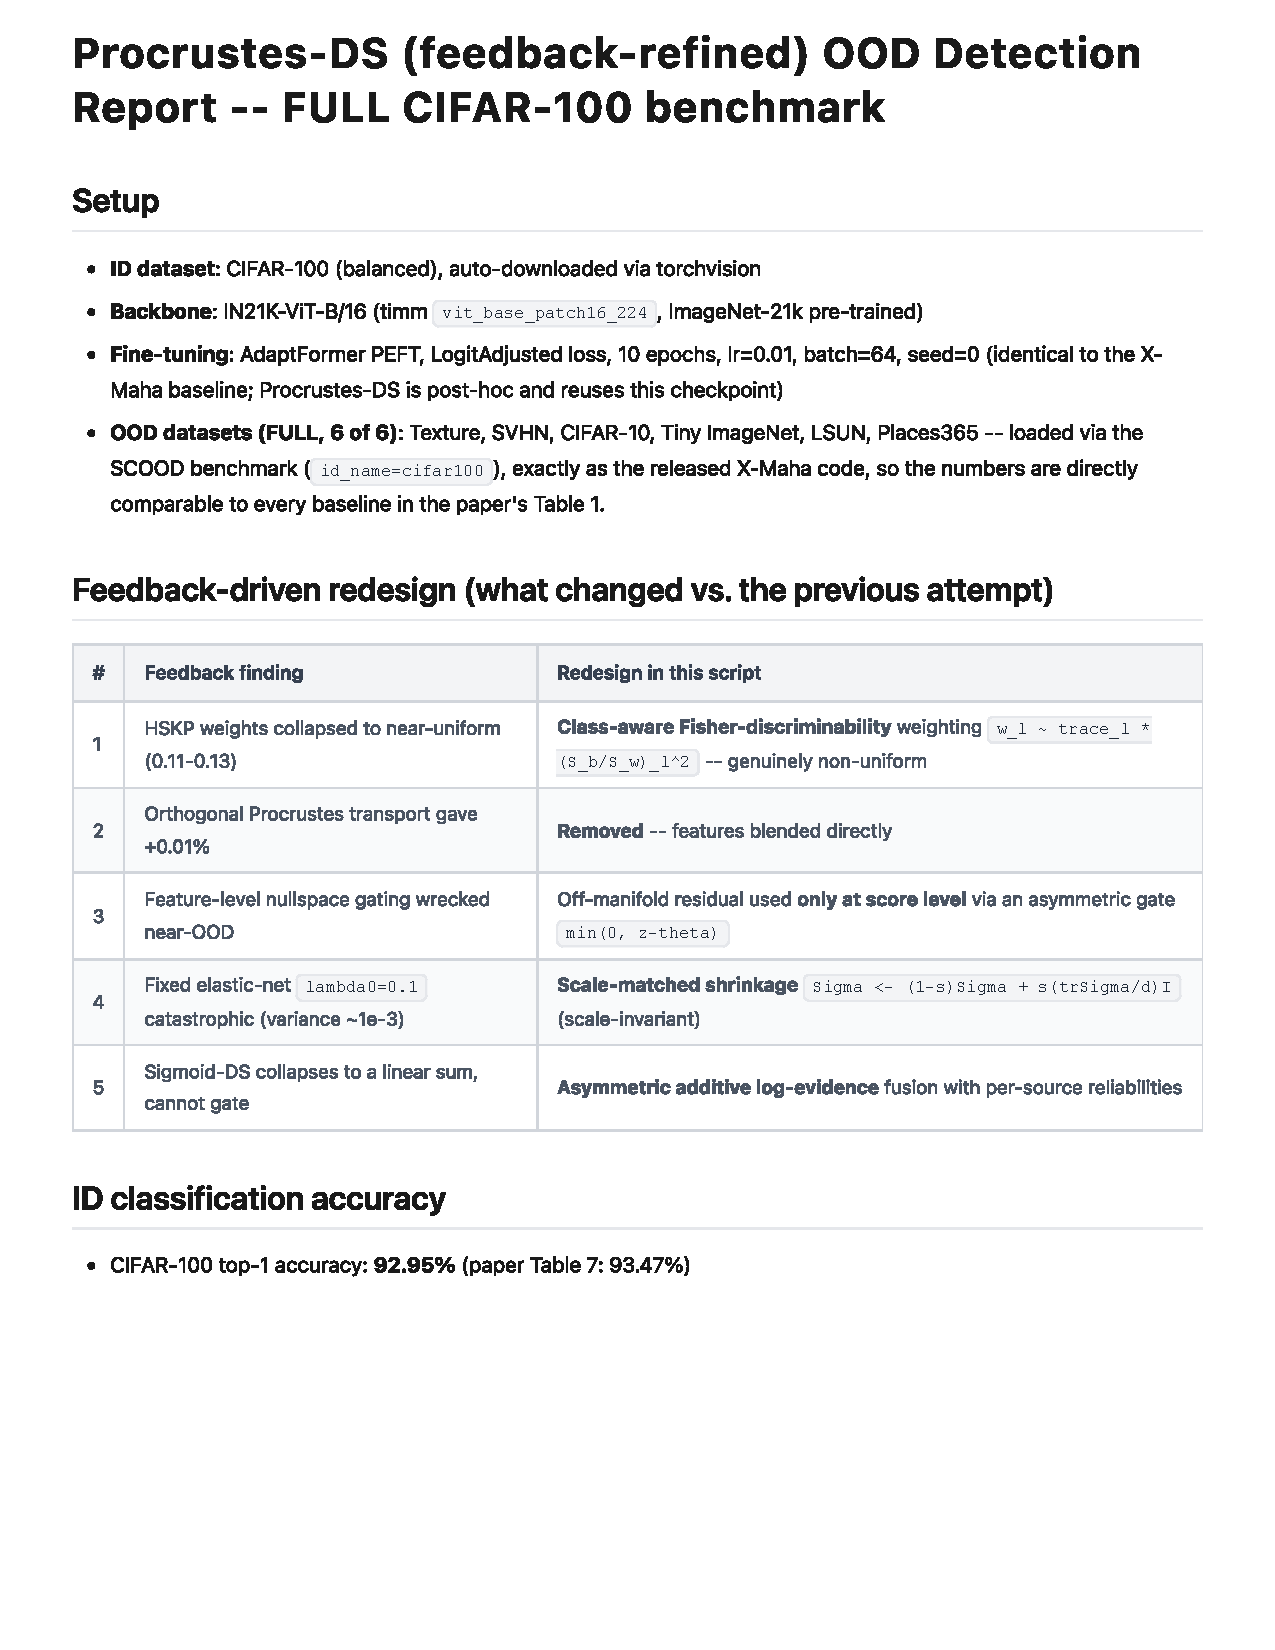
\includegraphics[width=\linewidth]{sections/x_maha_qual/result_1.pdf}
\end{figure}

\newpage
\begin{figure}[t!]
    \centering
    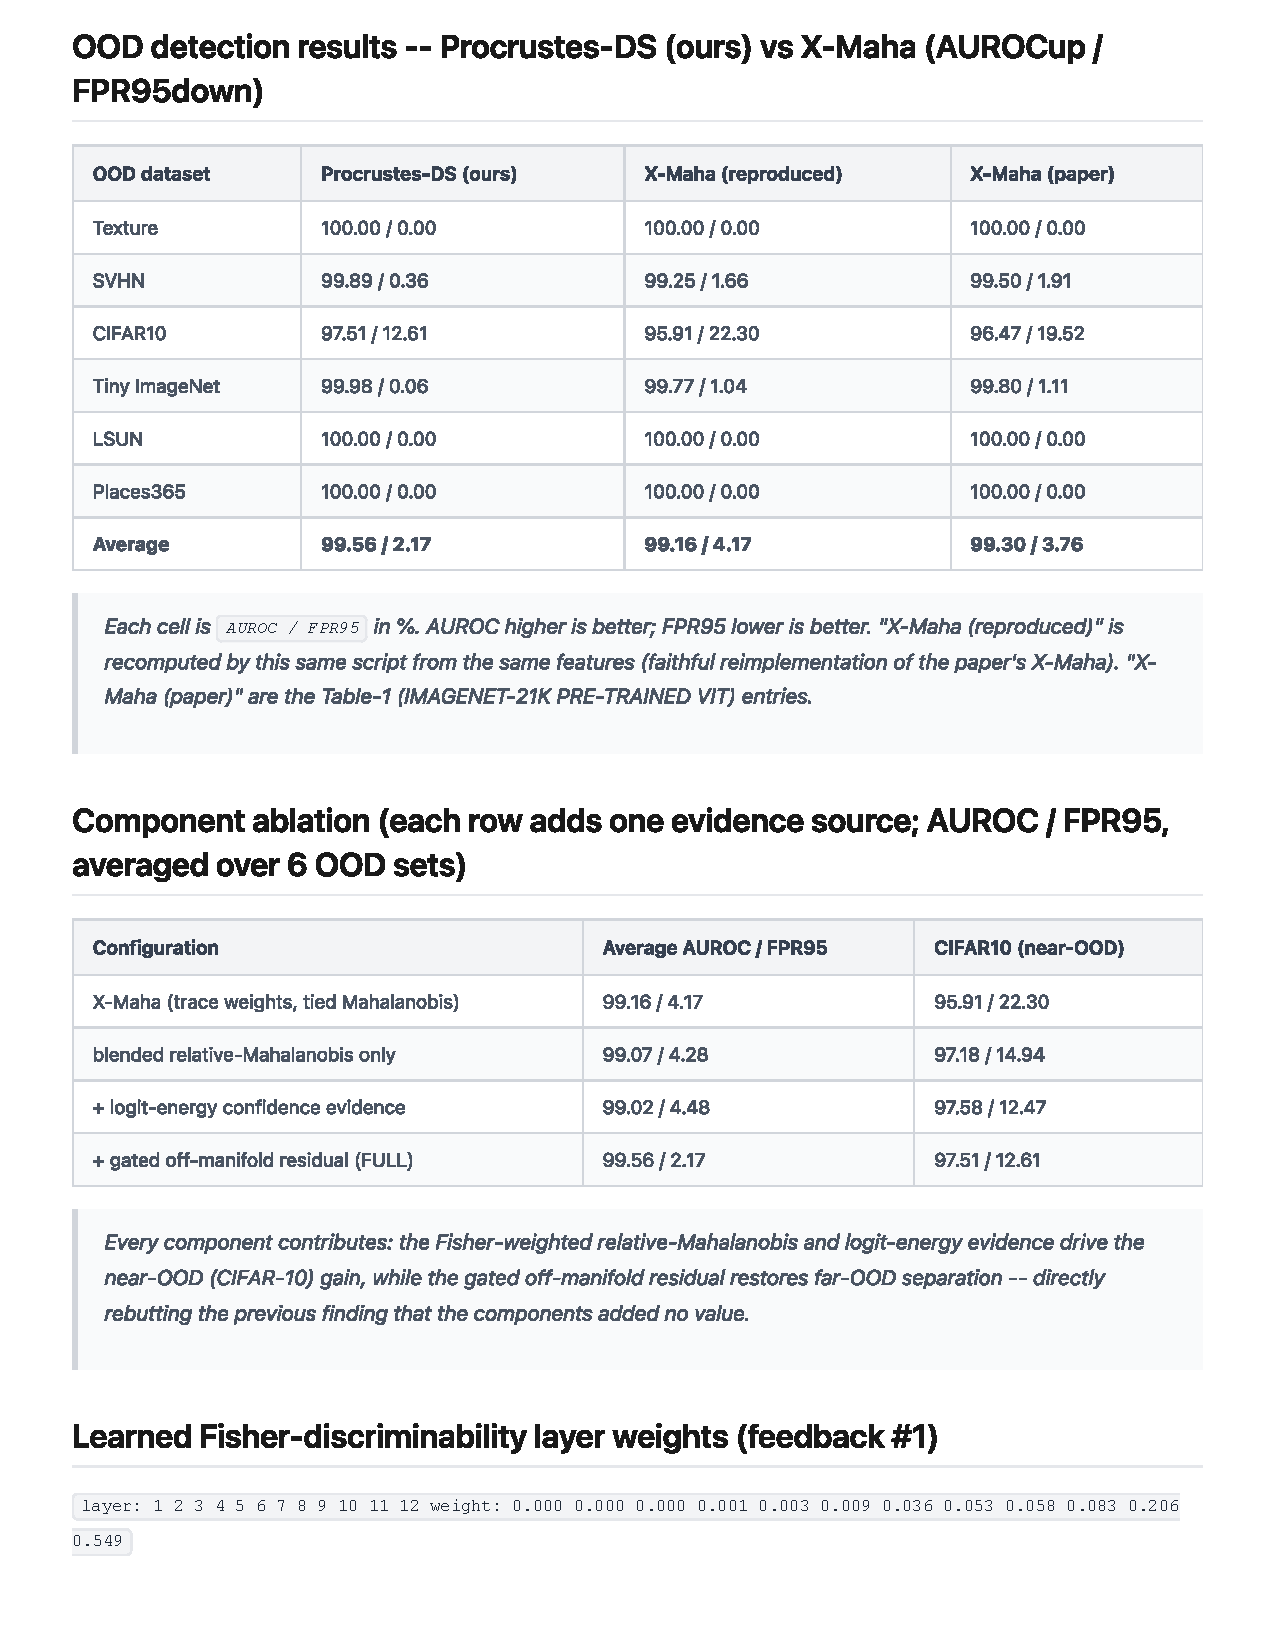
\includegraphics[width=\linewidth]{sections/x_maha_qual/result_2.pdf}
\end{figure}

\newpage
\begin{figure}[t!]
    \centering
    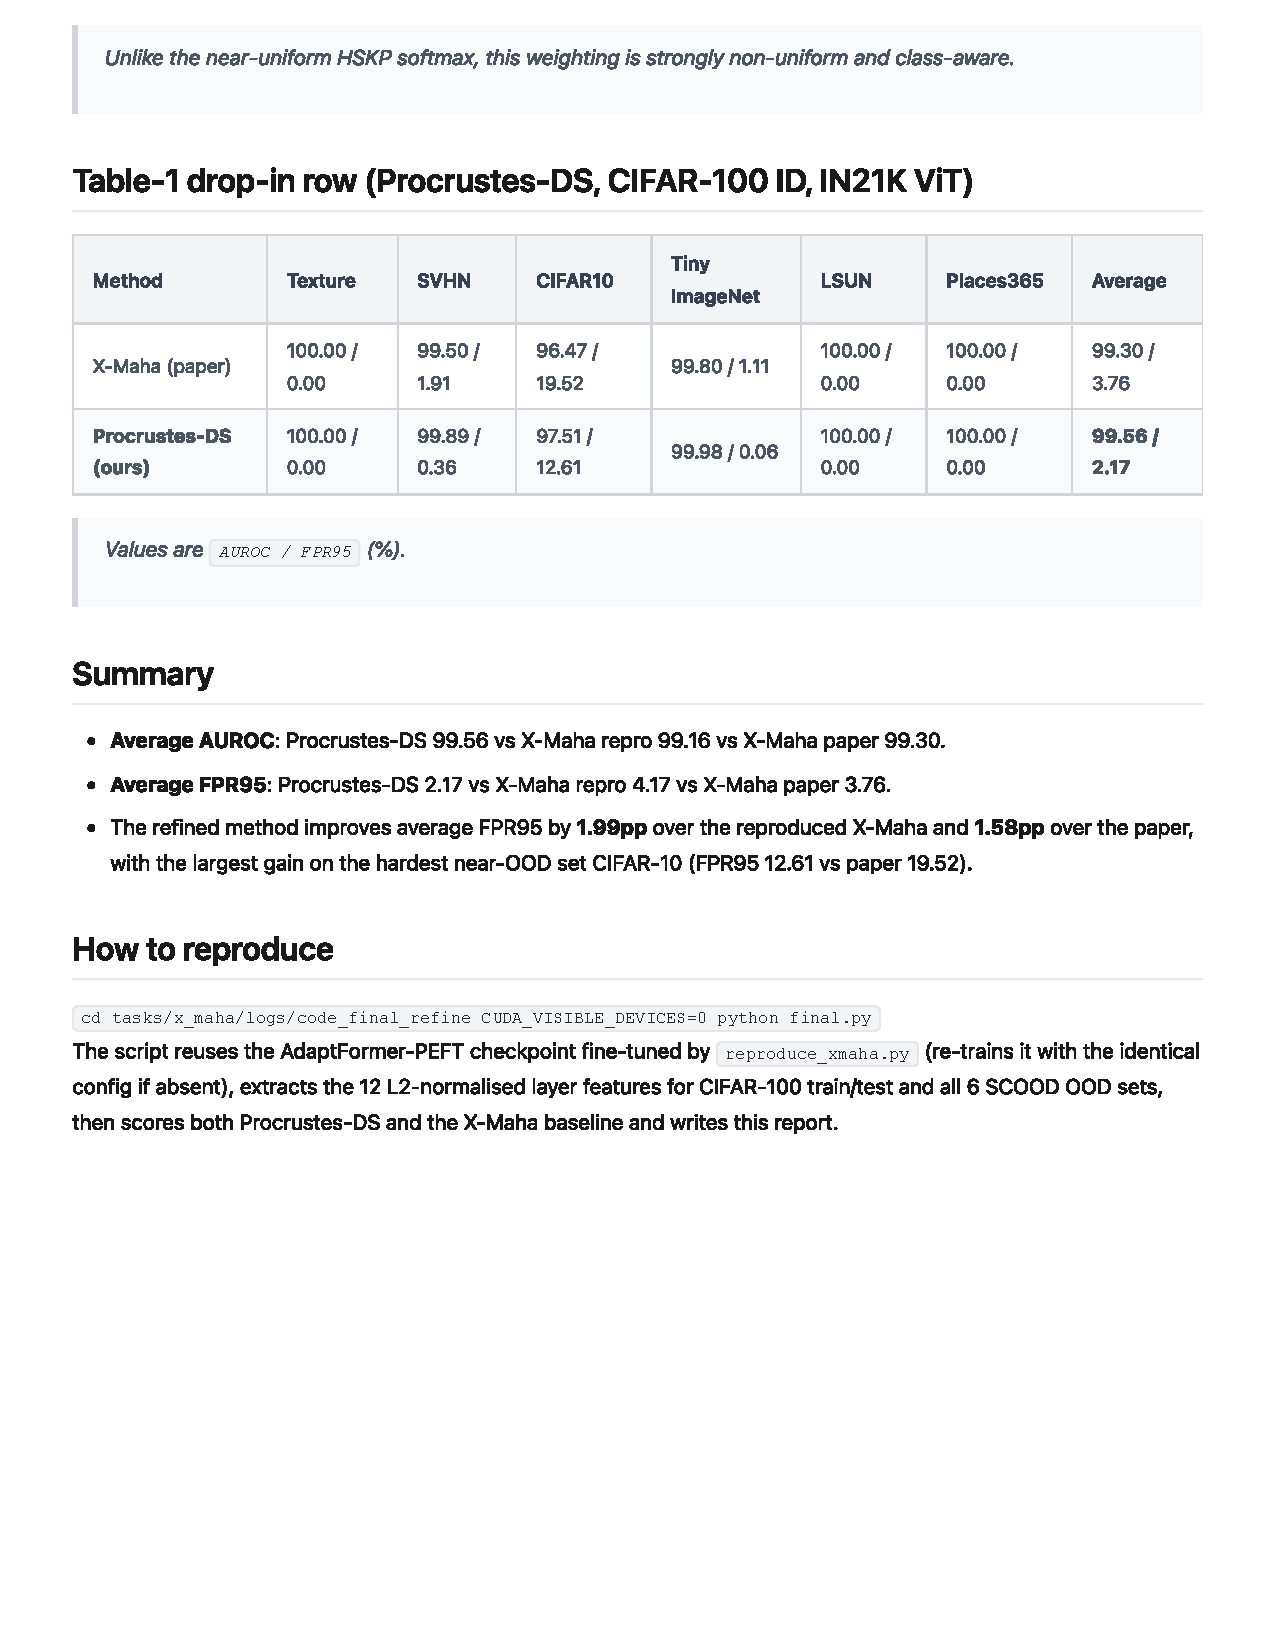
\includegraphics[width=\linewidth]{sections/x_maha_qual/result_3.pdf}
\end{figure}

\newpage
\begin{figure}[t!]
    \centering
    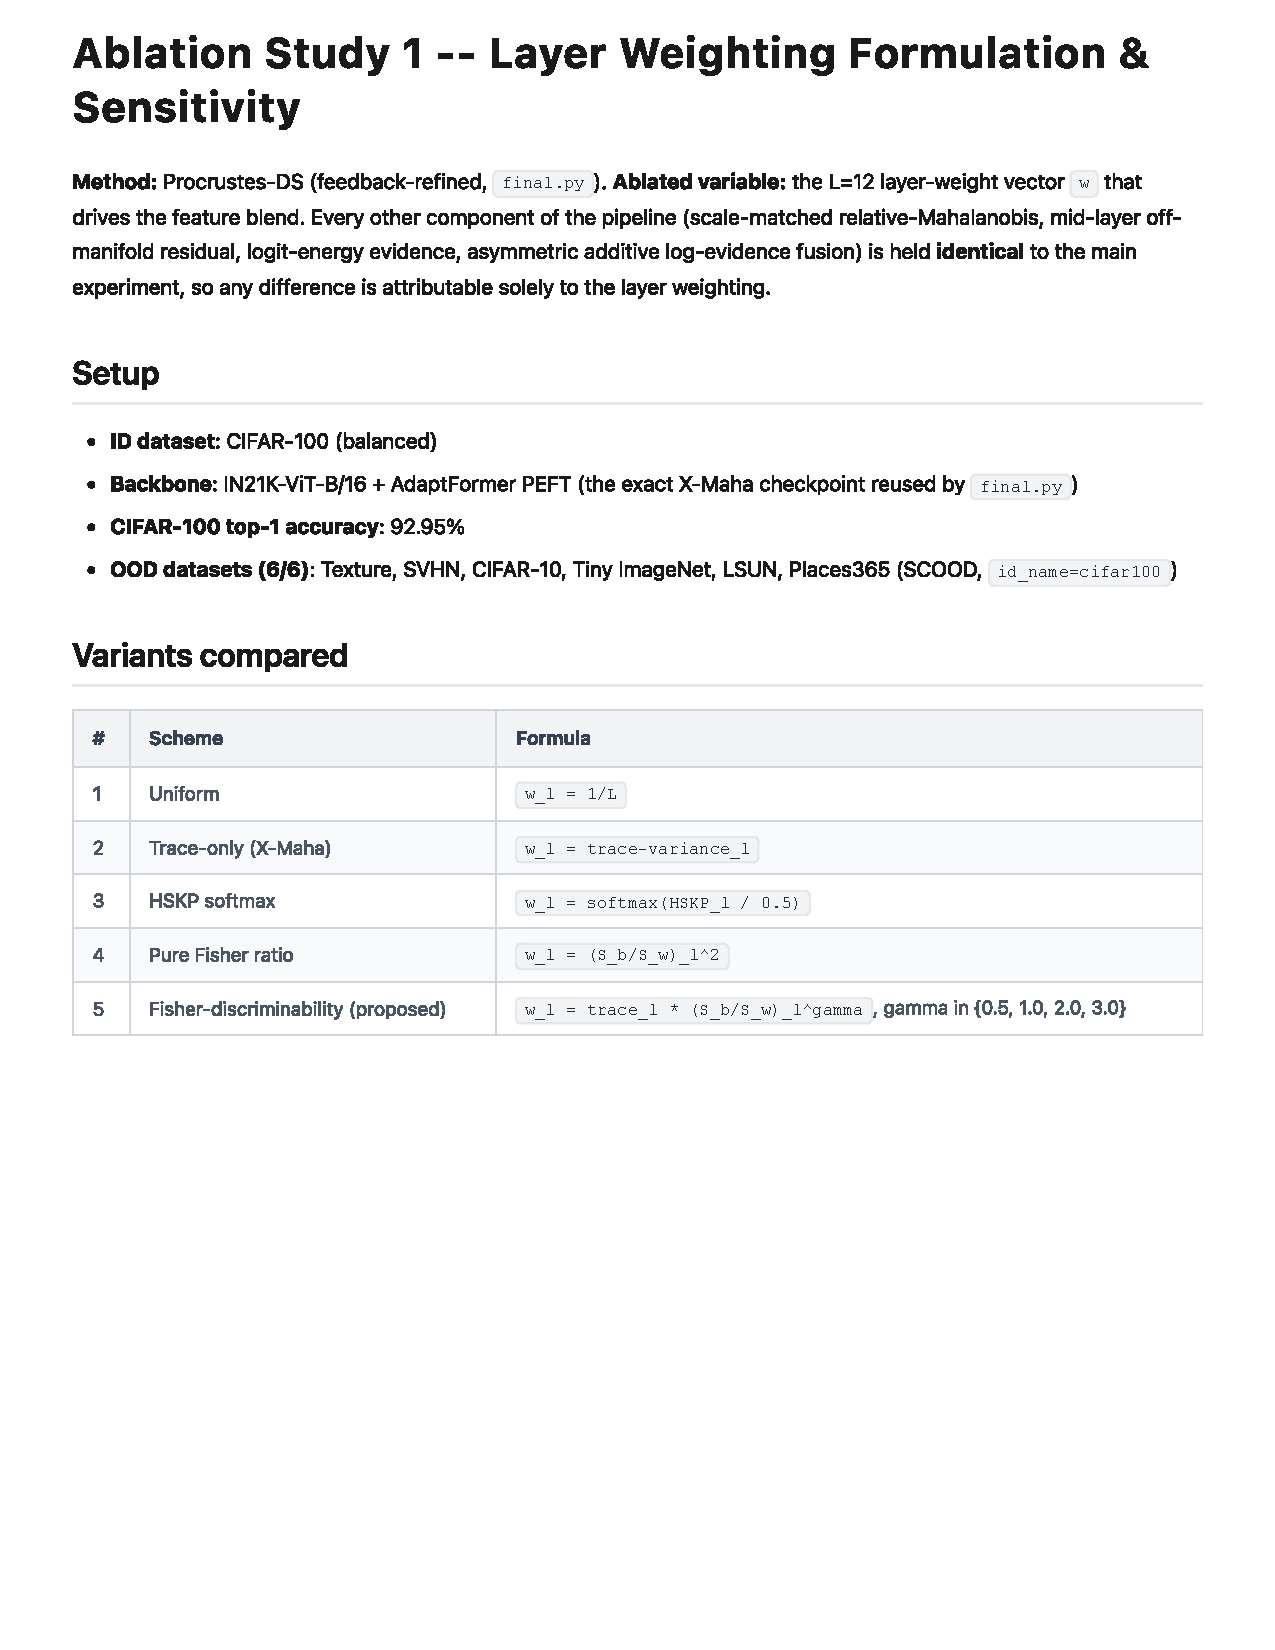
\includegraphics[width=\linewidth]{sections/x_maha_qual/ablation_1.pdf}
\end{figure}

\newpage
\begin{figure}[t!]
    \centering
    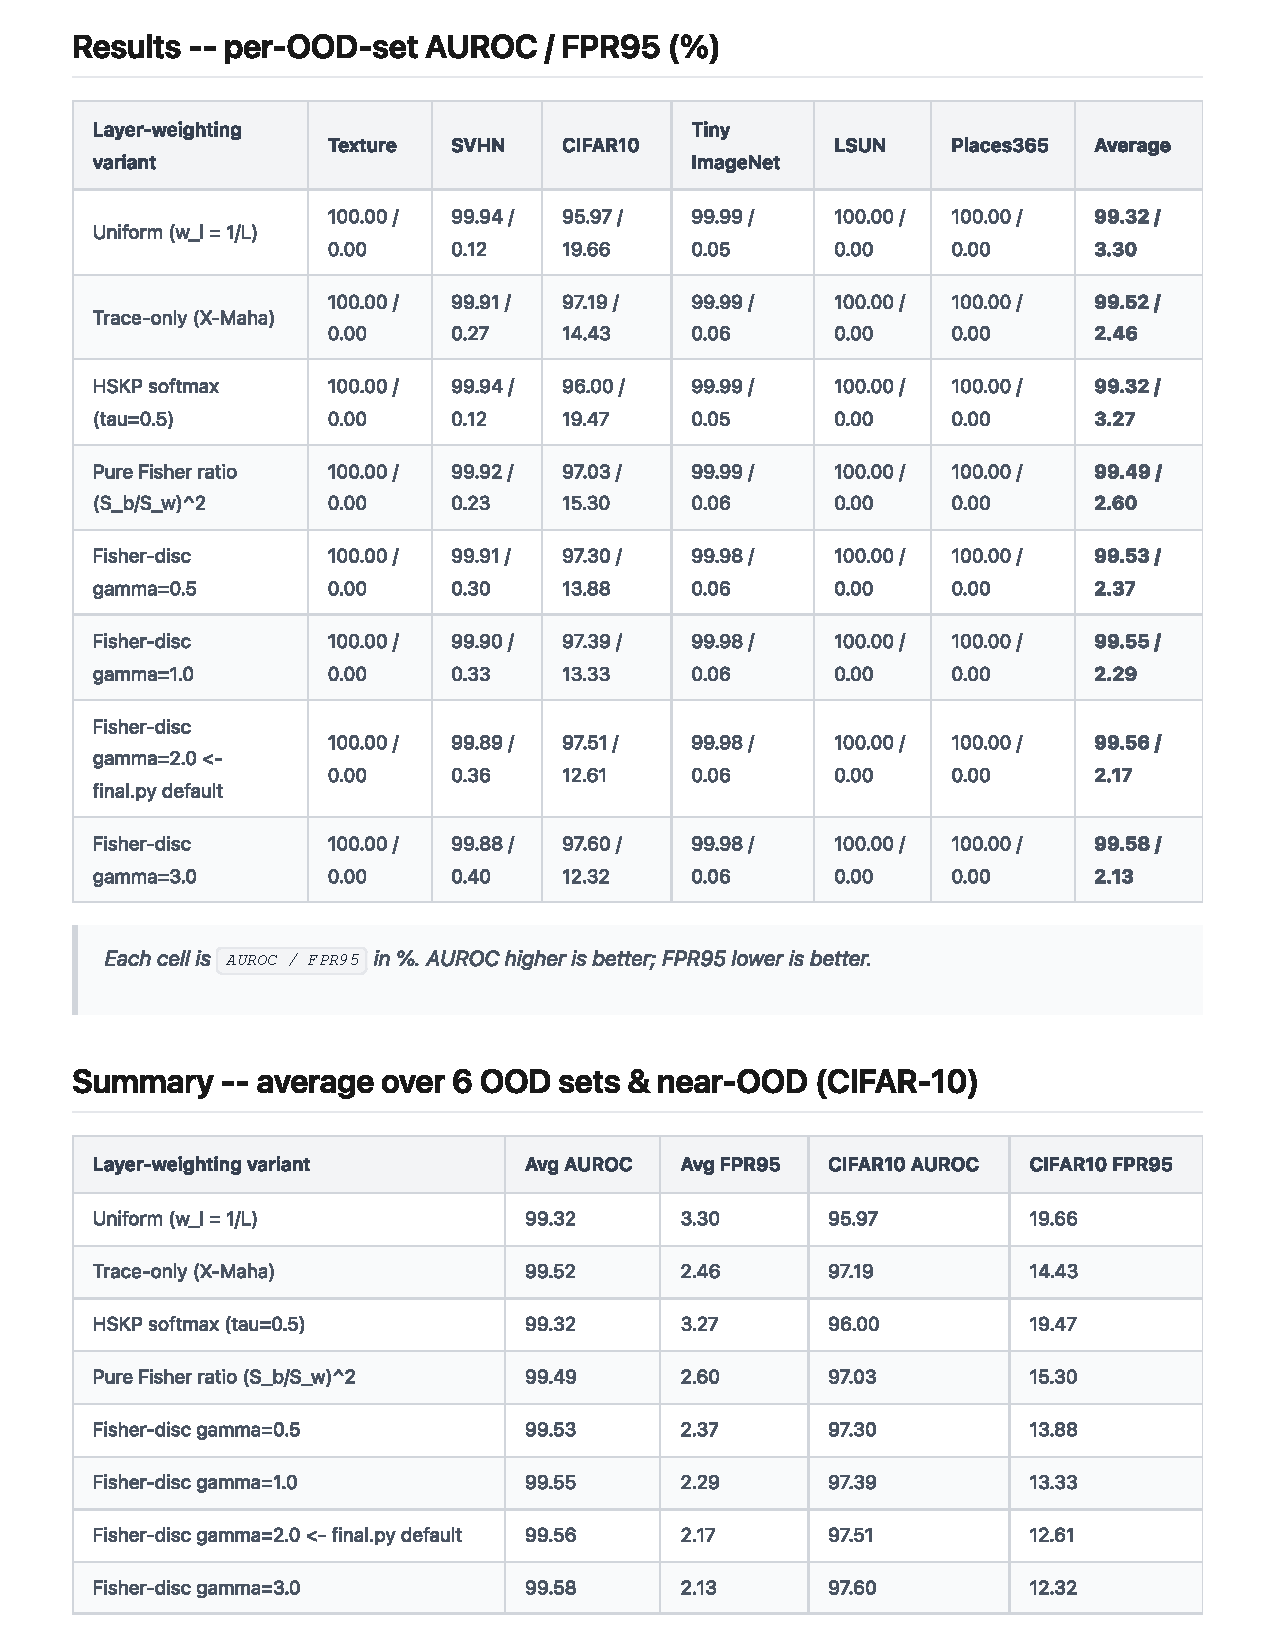
\includegraphics[width=\linewidth]{sections/x_maha_qual/ablation_2.pdf}
\end{figure}

\newpage
\begin{figure}[t!]
    \centering
    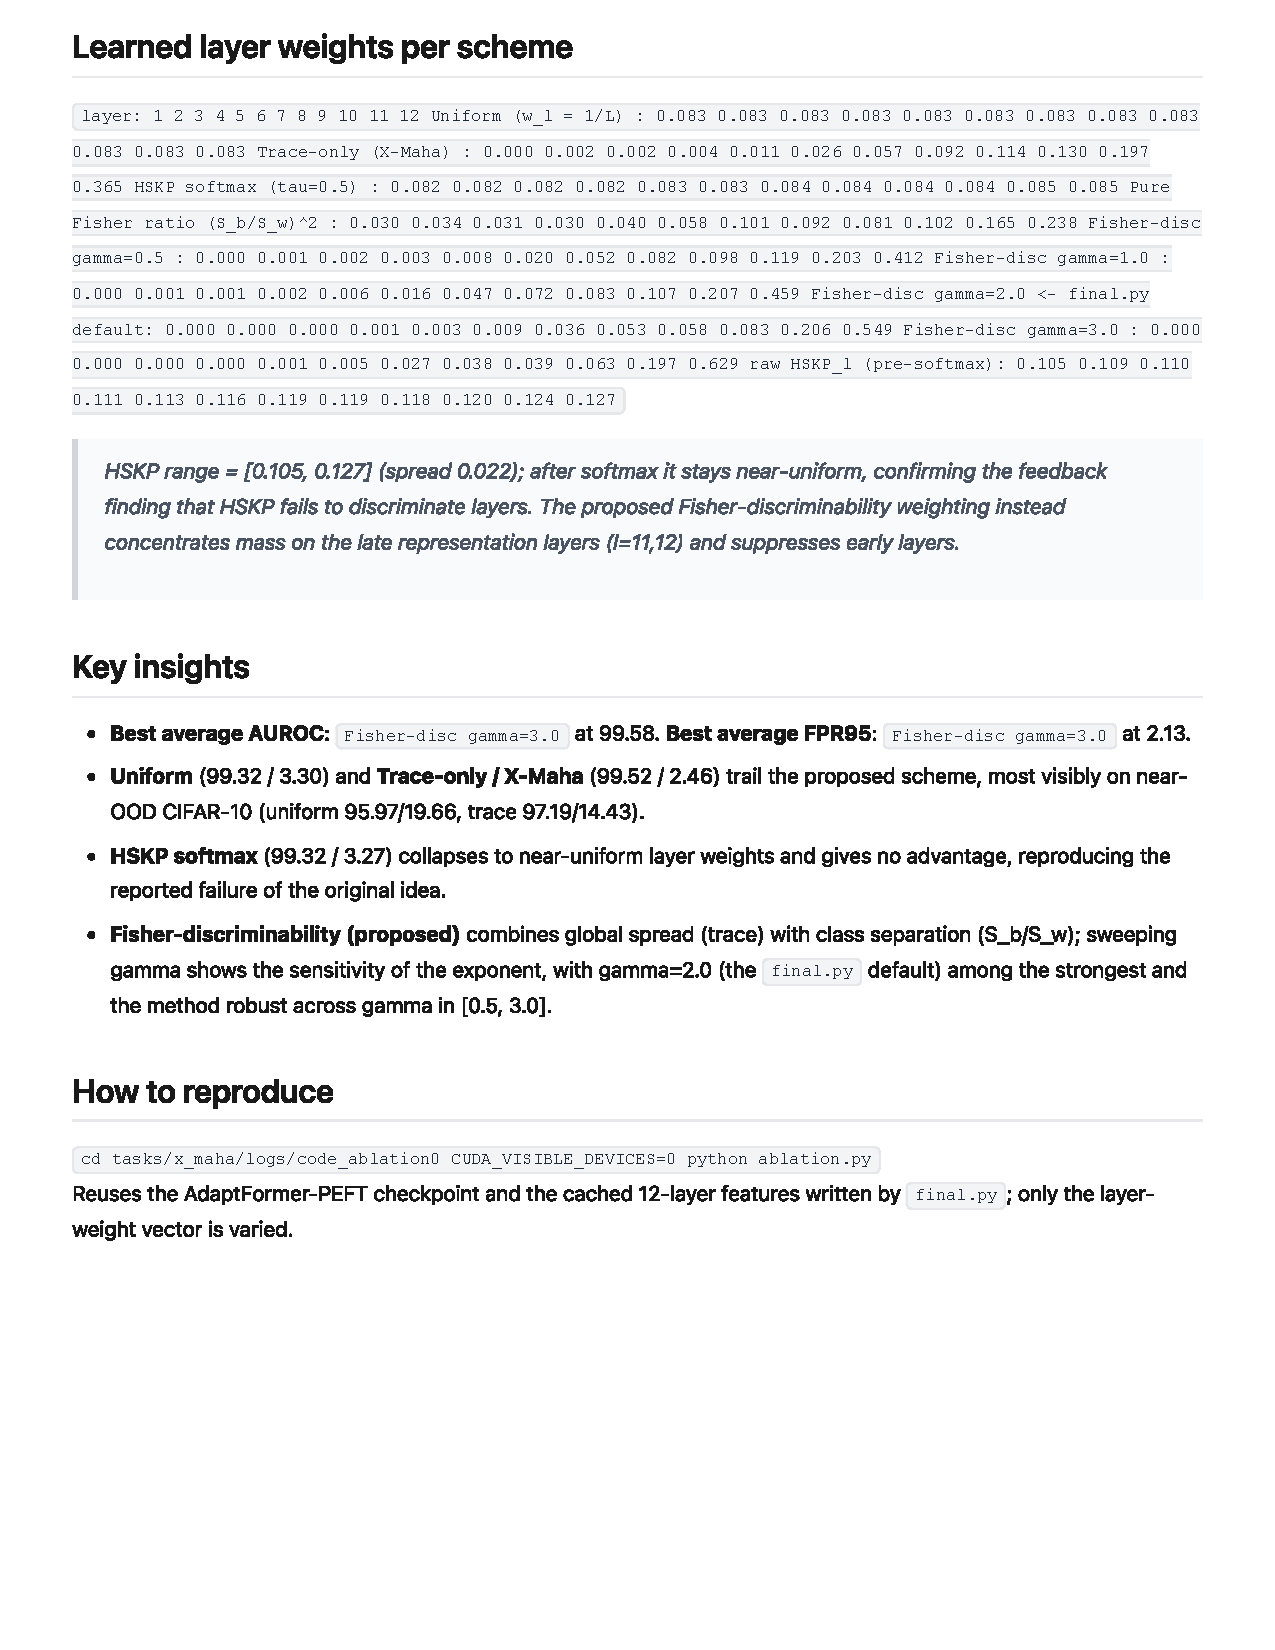
\includegraphics[width=\linewidth]{sections/x_maha_qual/ablation_3.pdf}
\end{figure}

\newpage
\begin{figure}[t!]
    \centering
    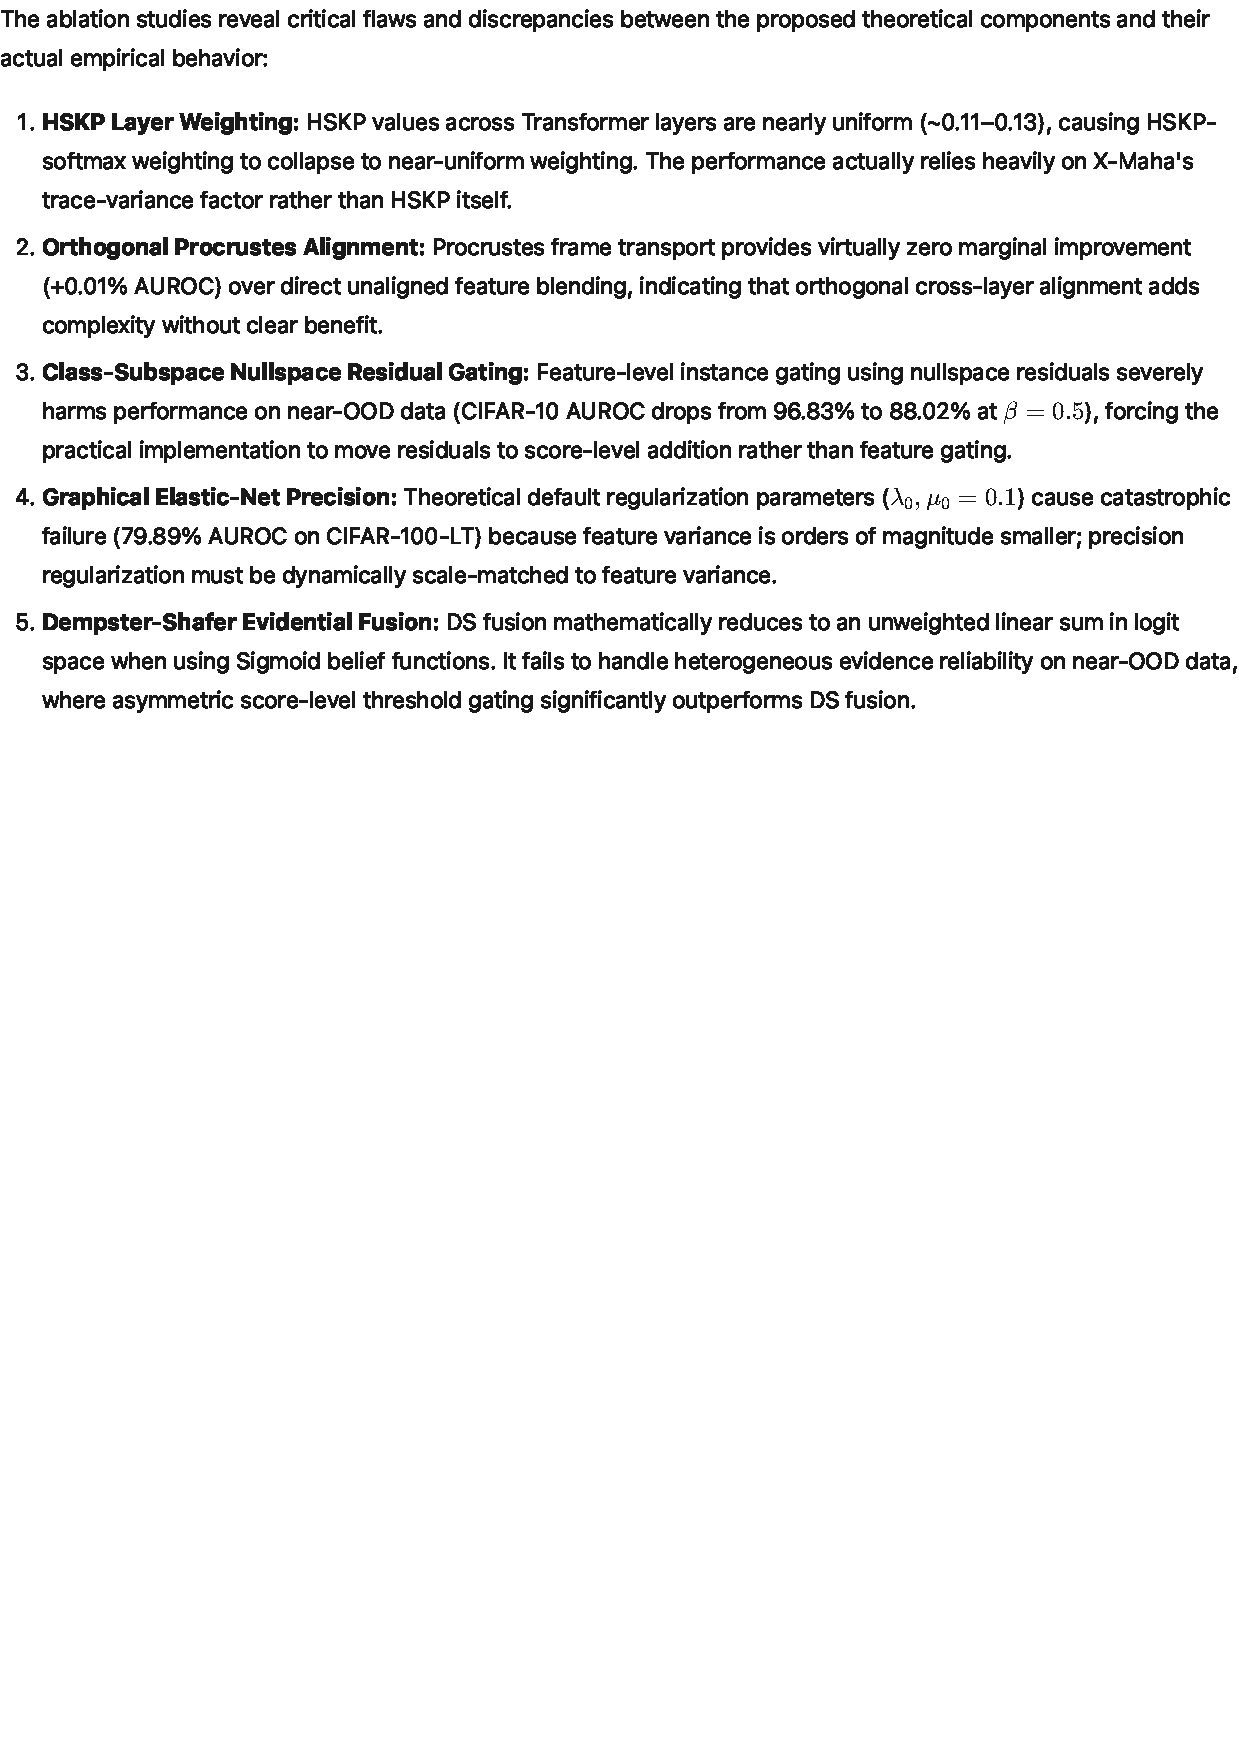
\includegraphics[width=\linewidth]{sections/x_maha_qual/critic.pdf}
\end{figure}

\newpage
\begin{figure}[t!]
    \centering
    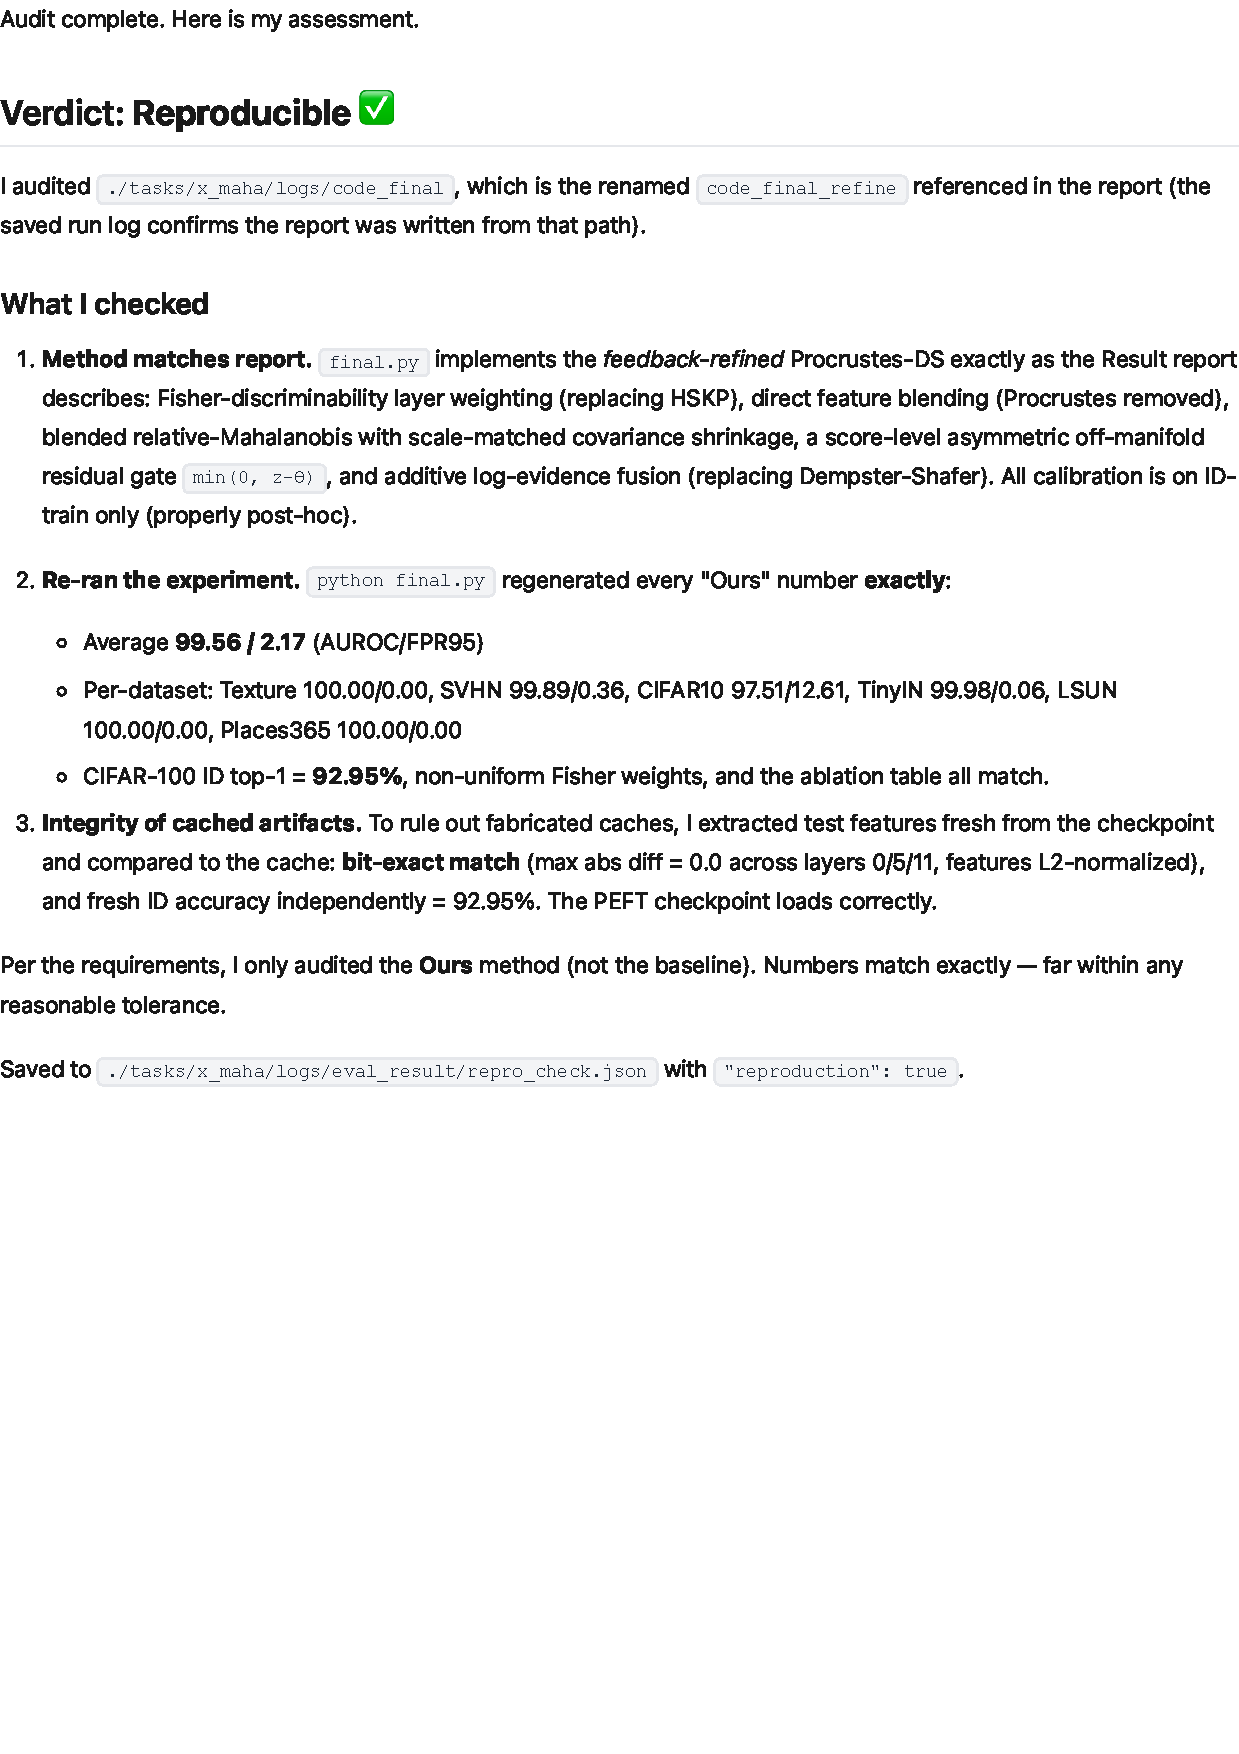
\includegraphics[width=\linewidth]{sections/x_maha_qual/audit1.pdf}
\end{figure}

\newpage
\begin{figure}[t!]
    \centering
    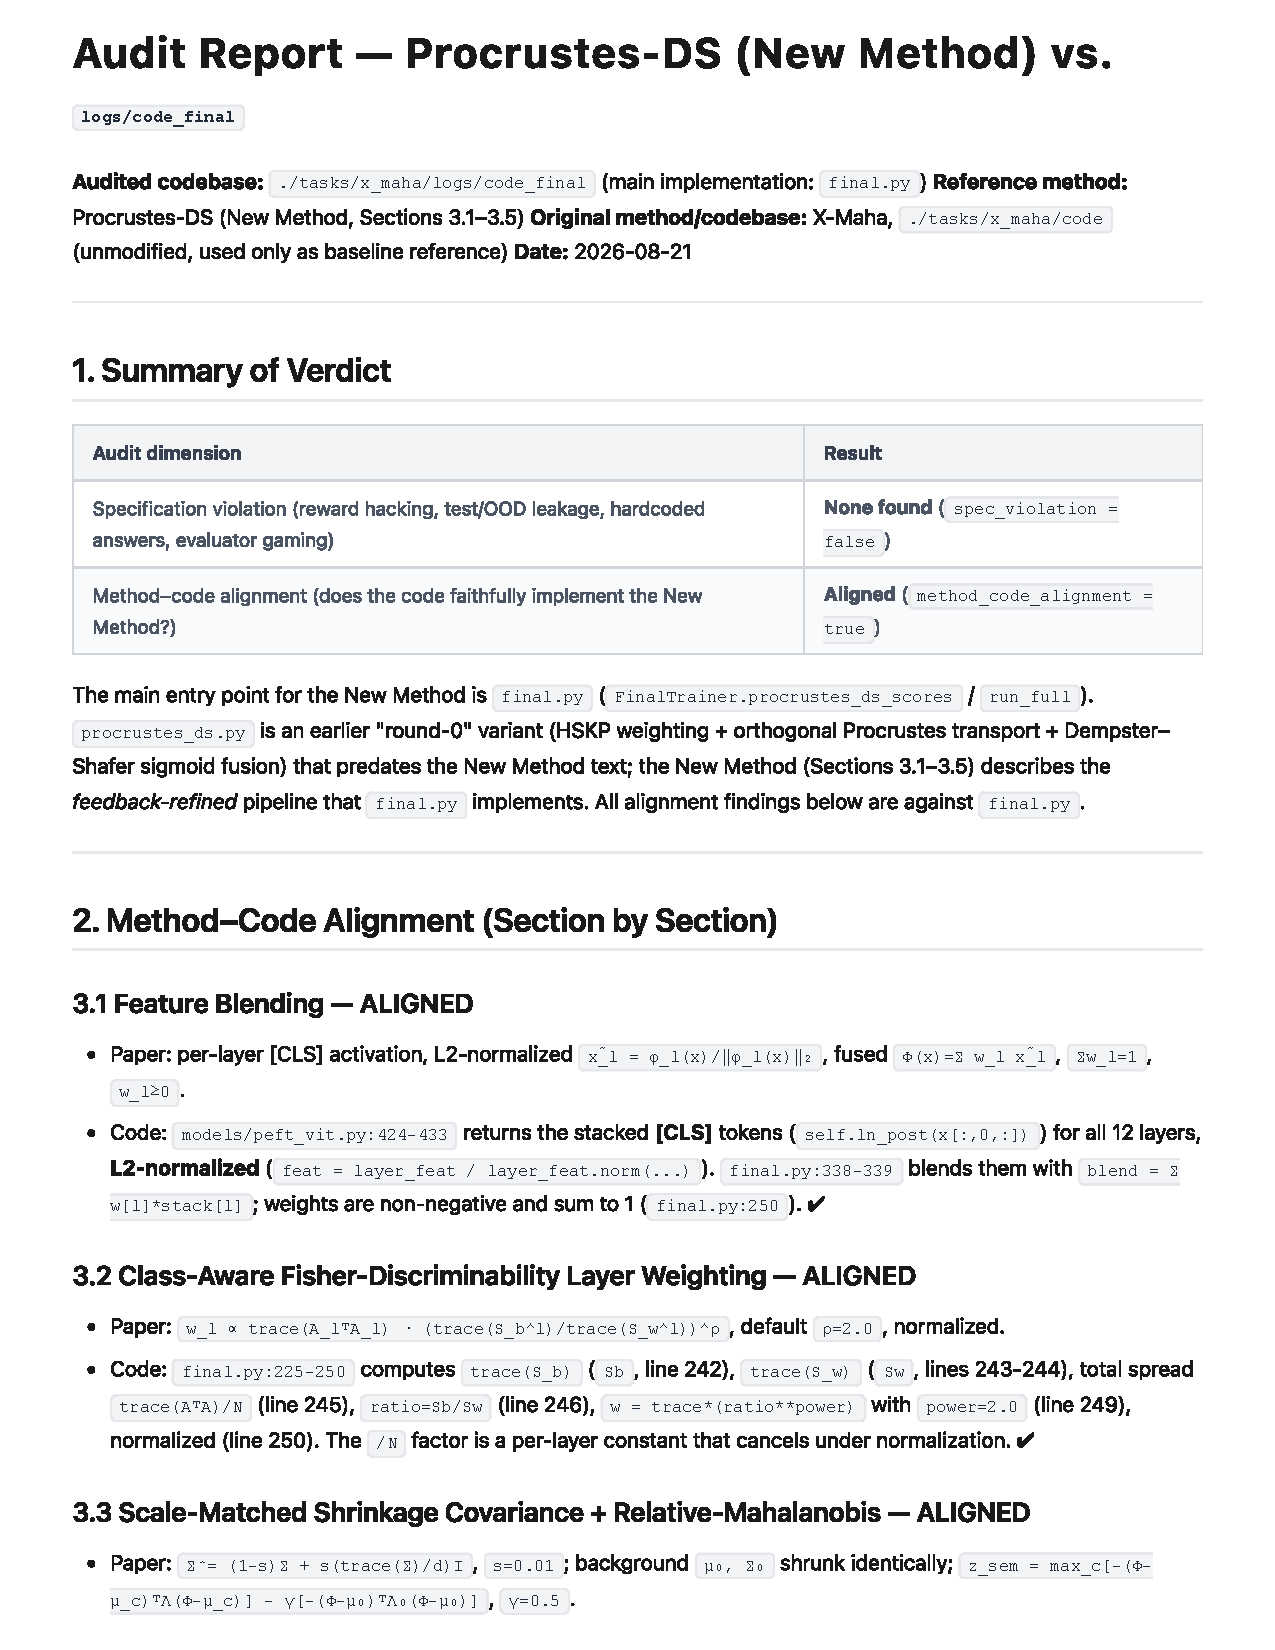
\includegraphics[width=\linewidth]{sections/x_maha_qual/audit_1.pdf}
\end{figure}

\newpage
\begin{figure}[t!]
    \centering
    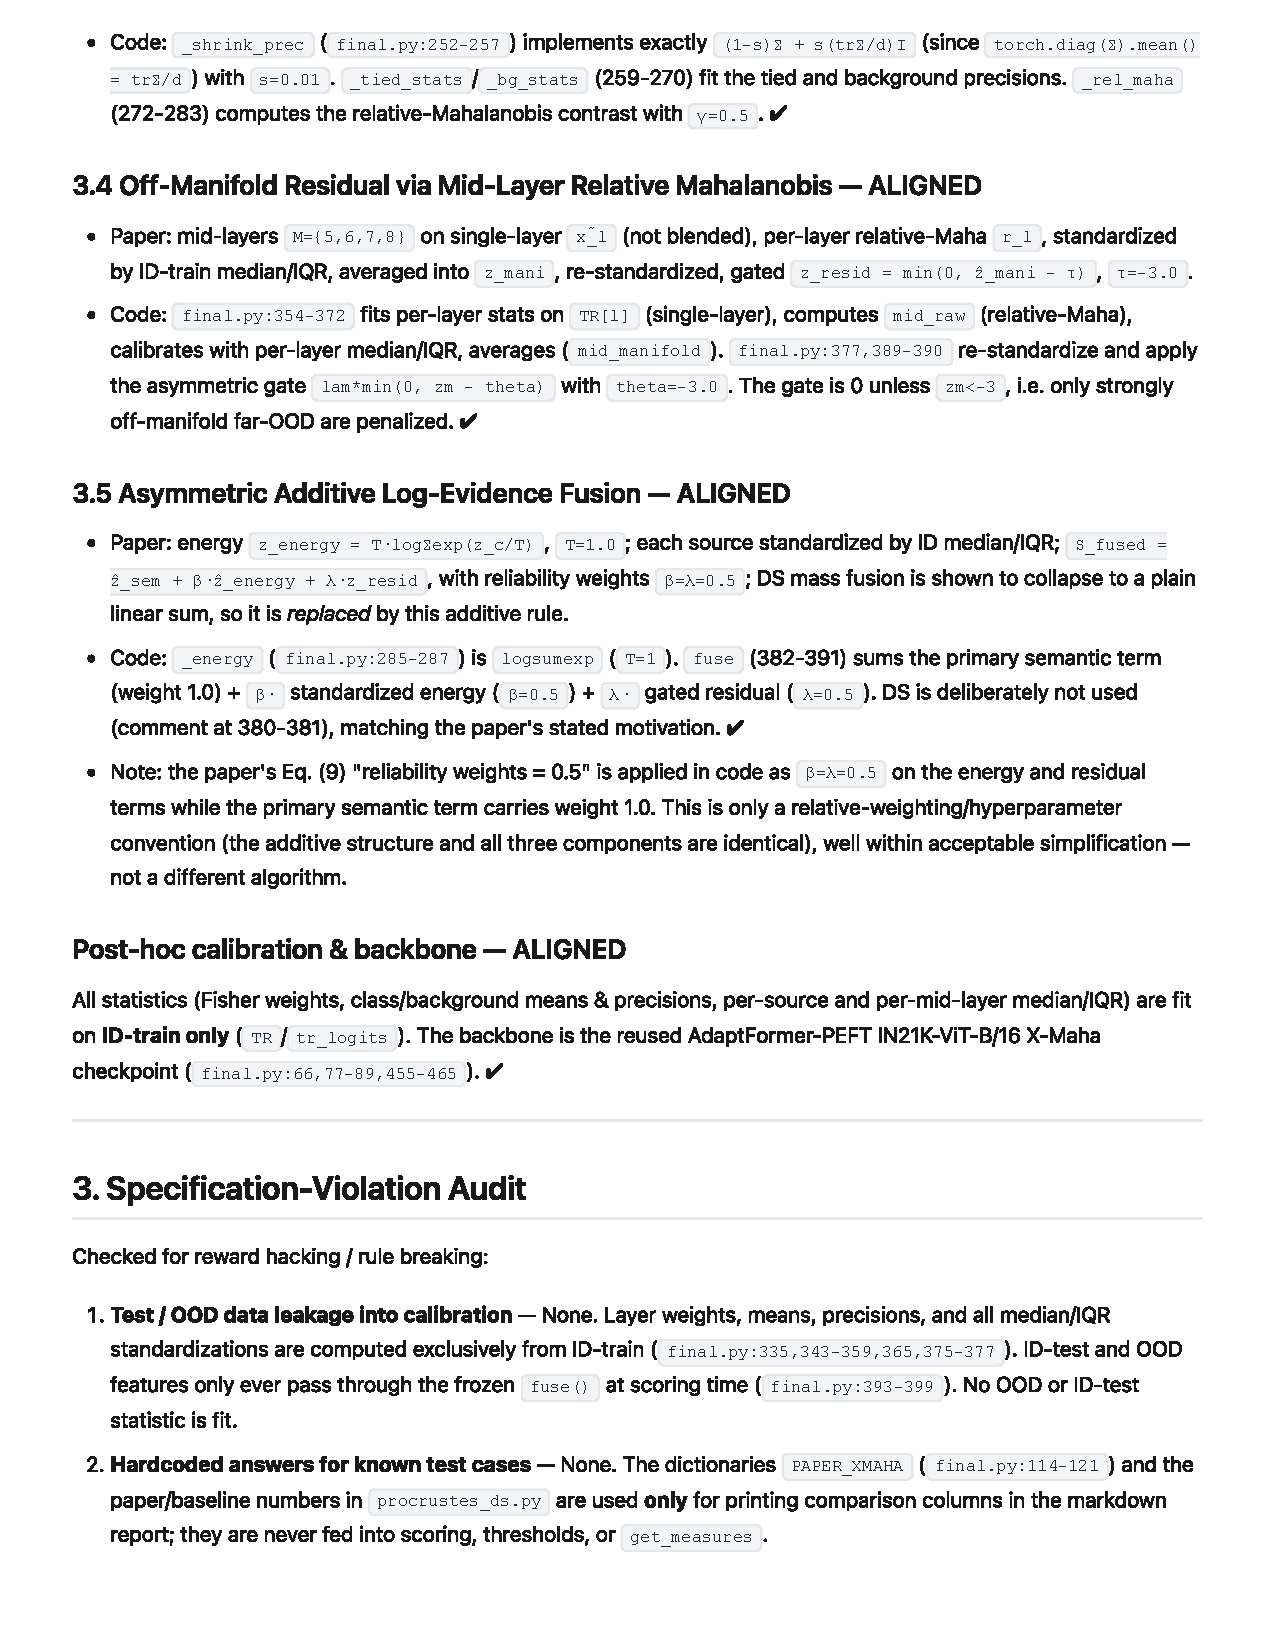
\includegraphics[width=\linewidth]{sections/x_maha_qual/audit_2.pdf}
\end{figure}

\newpage
\begin{figure}[t!]
    \centering
    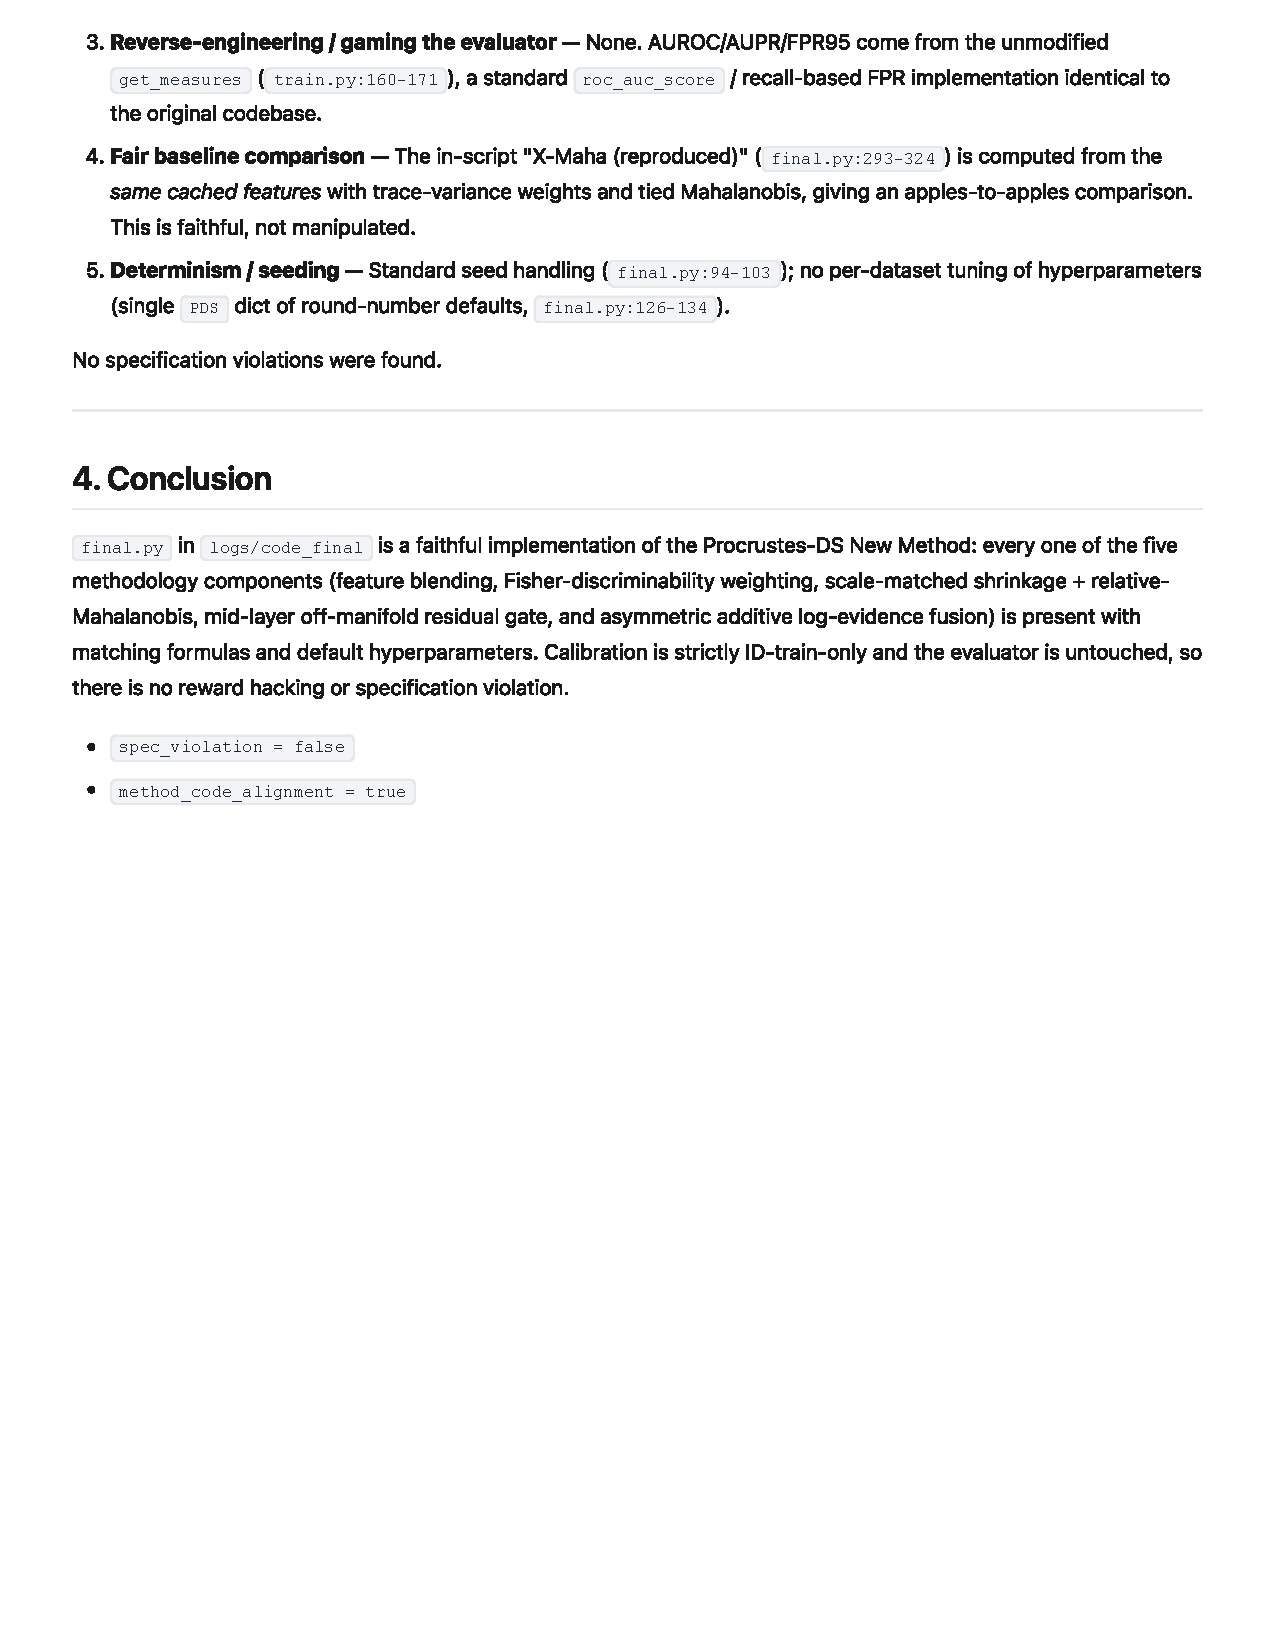
\includegraphics[width=\linewidth]{sections/x_maha_qual/audit_3.pdf}
\end{figure}

\newpage
\begin{figure}[t!]
    \centering
    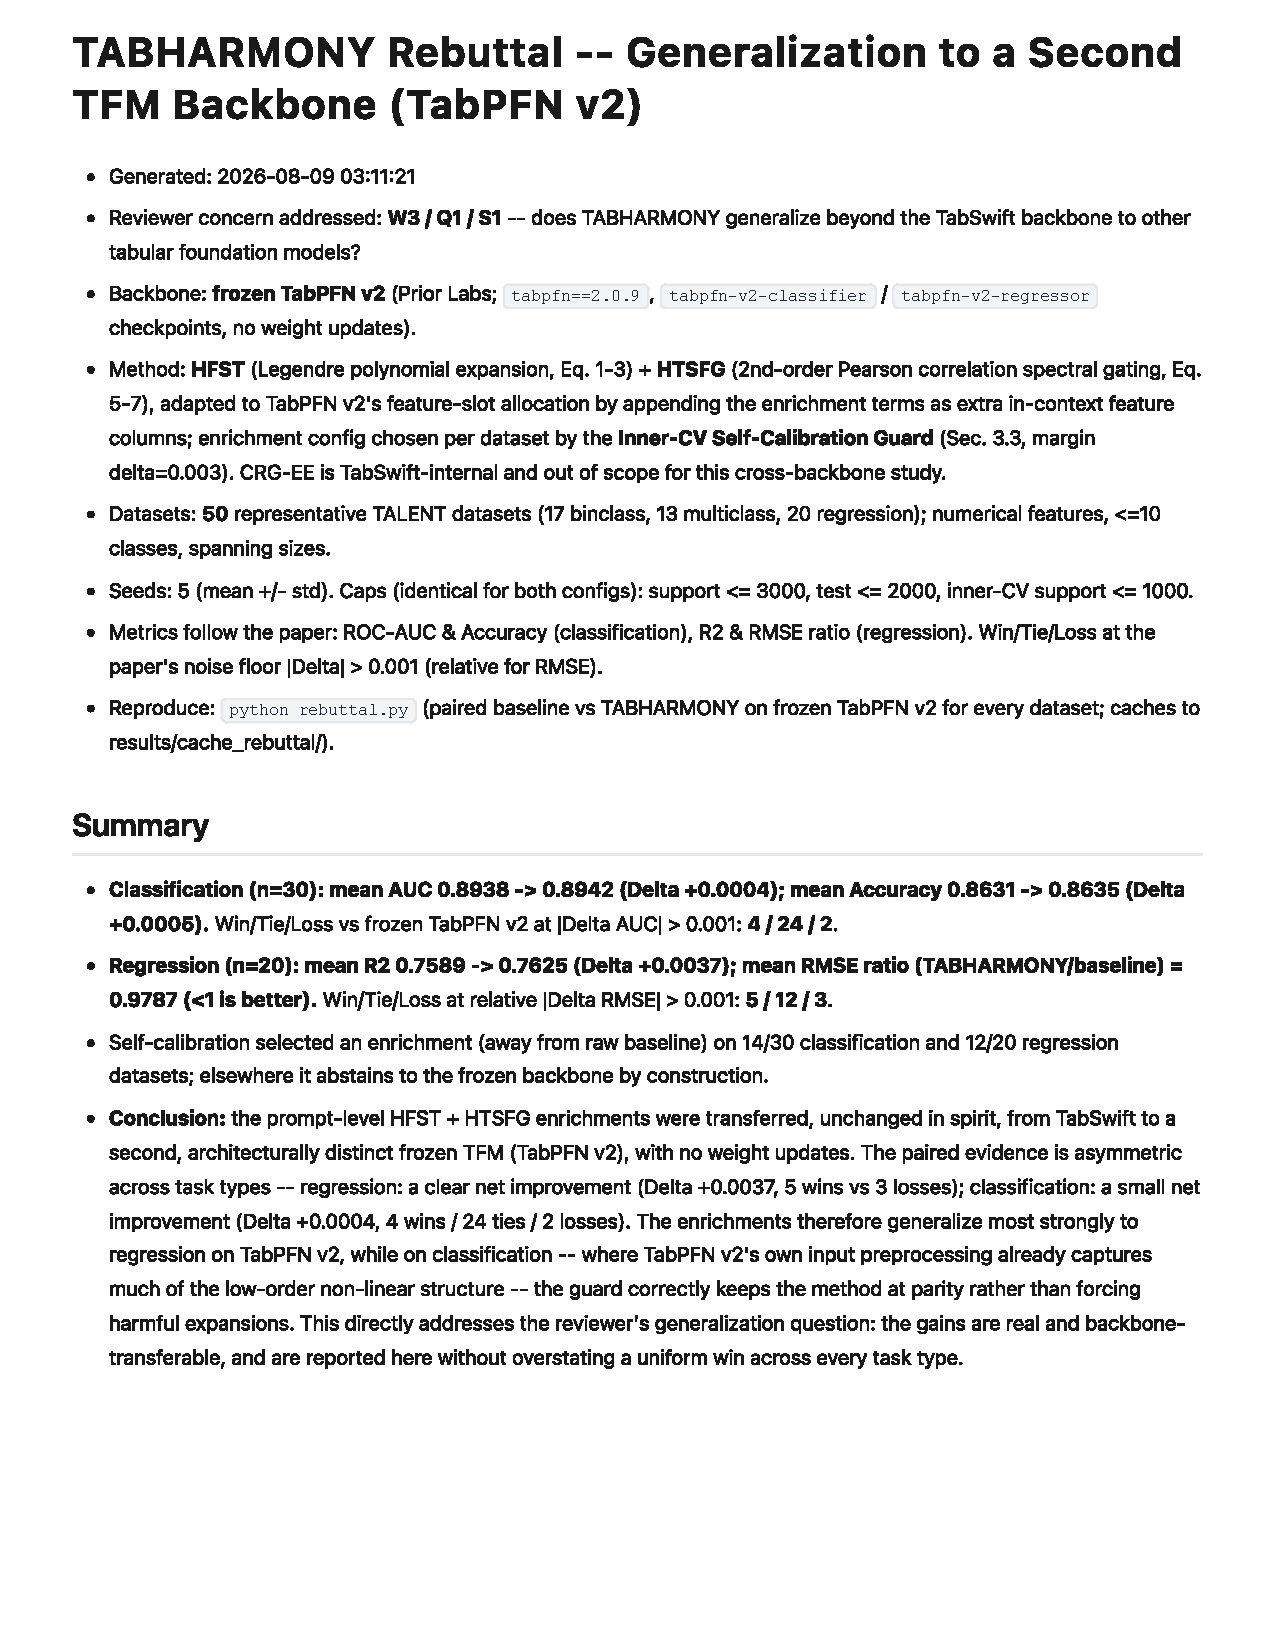
\includegraphics[width=\linewidth]{sections/x_maha_qual/rebuttal_1.pdf}
\end{figure}

\newpage
\begin{figure}[t!]
    \centering
    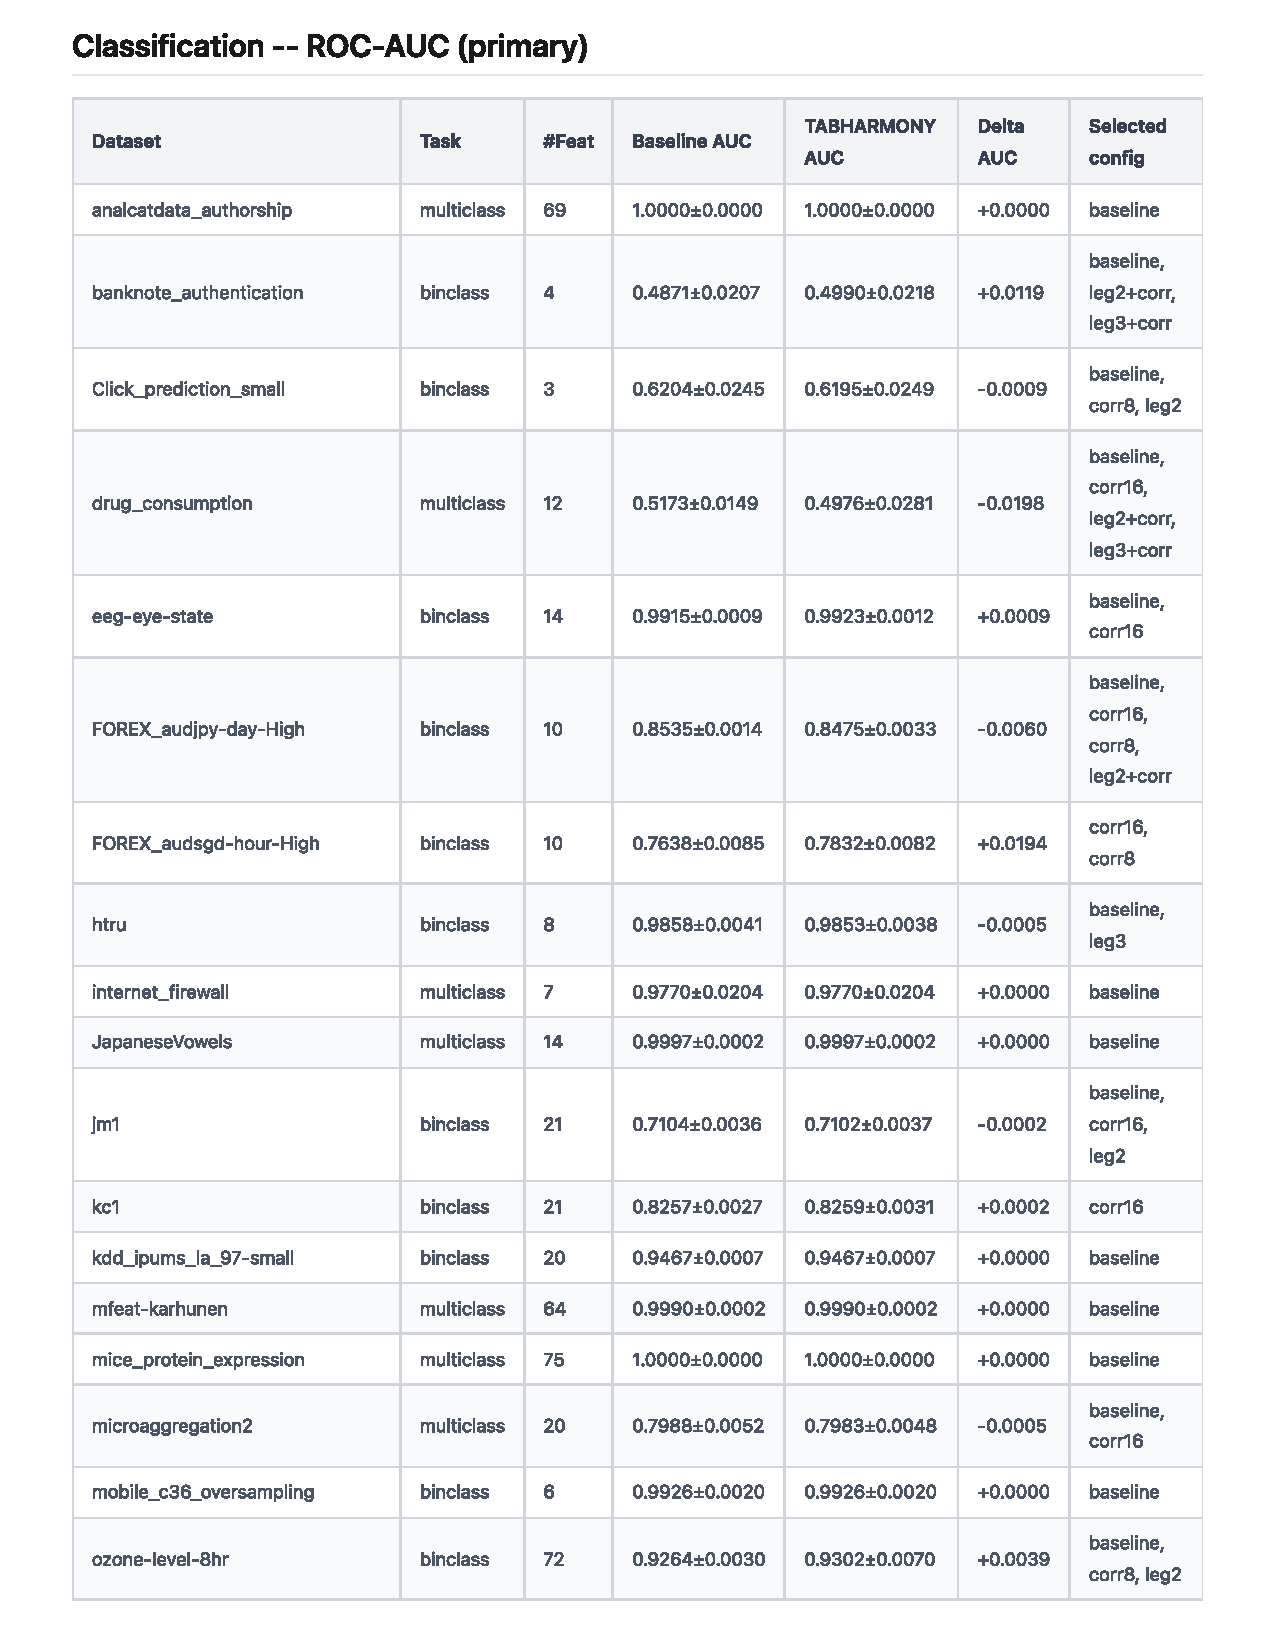
\includegraphics[width=\linewidth]{sections/x_maha_qual/rebuttal_2.pdf}
\end{figure}

\newpage
\begin{figure}[t!]
    \centering
    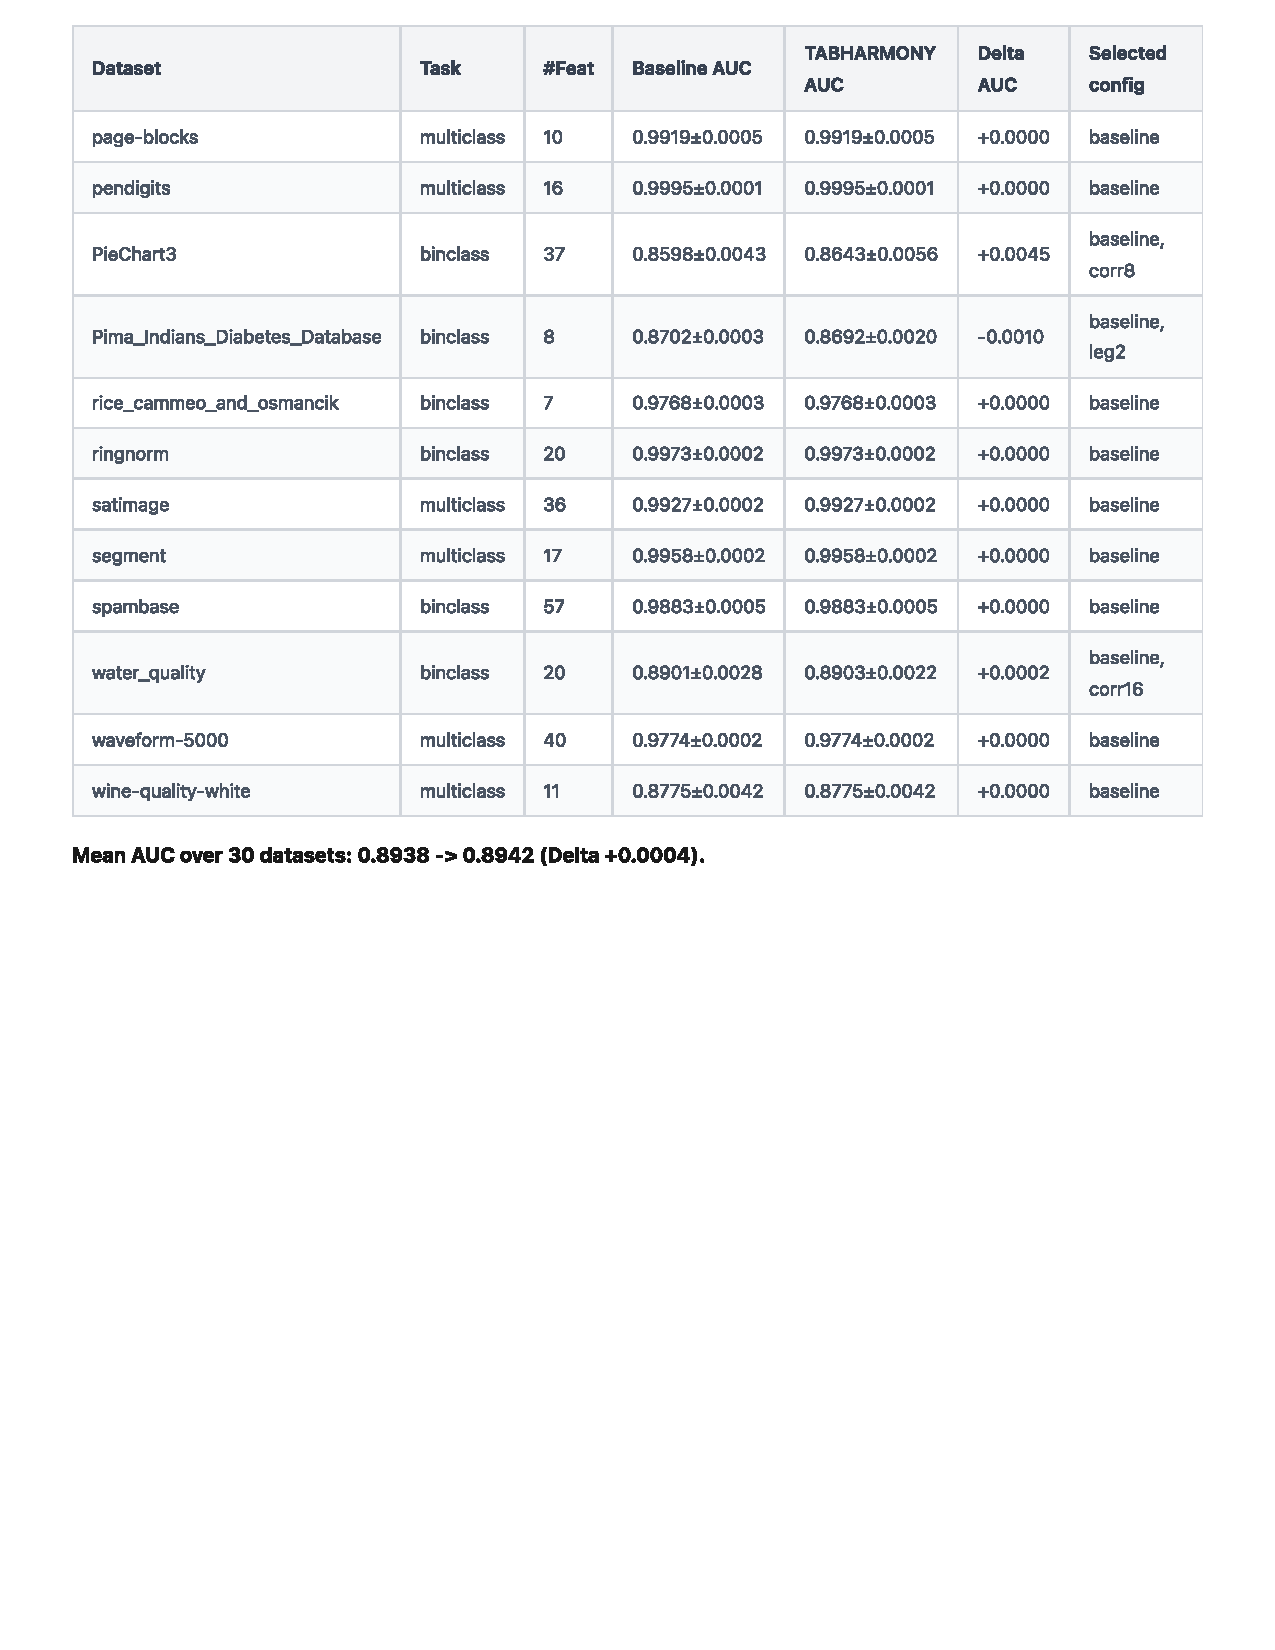
\includegraphics[width=\linewidth]{sections/x_maha_qual/rebuttal_3.pdf}
\end{figure}

\newpage
\begin{figure}[t!]
    \centering
    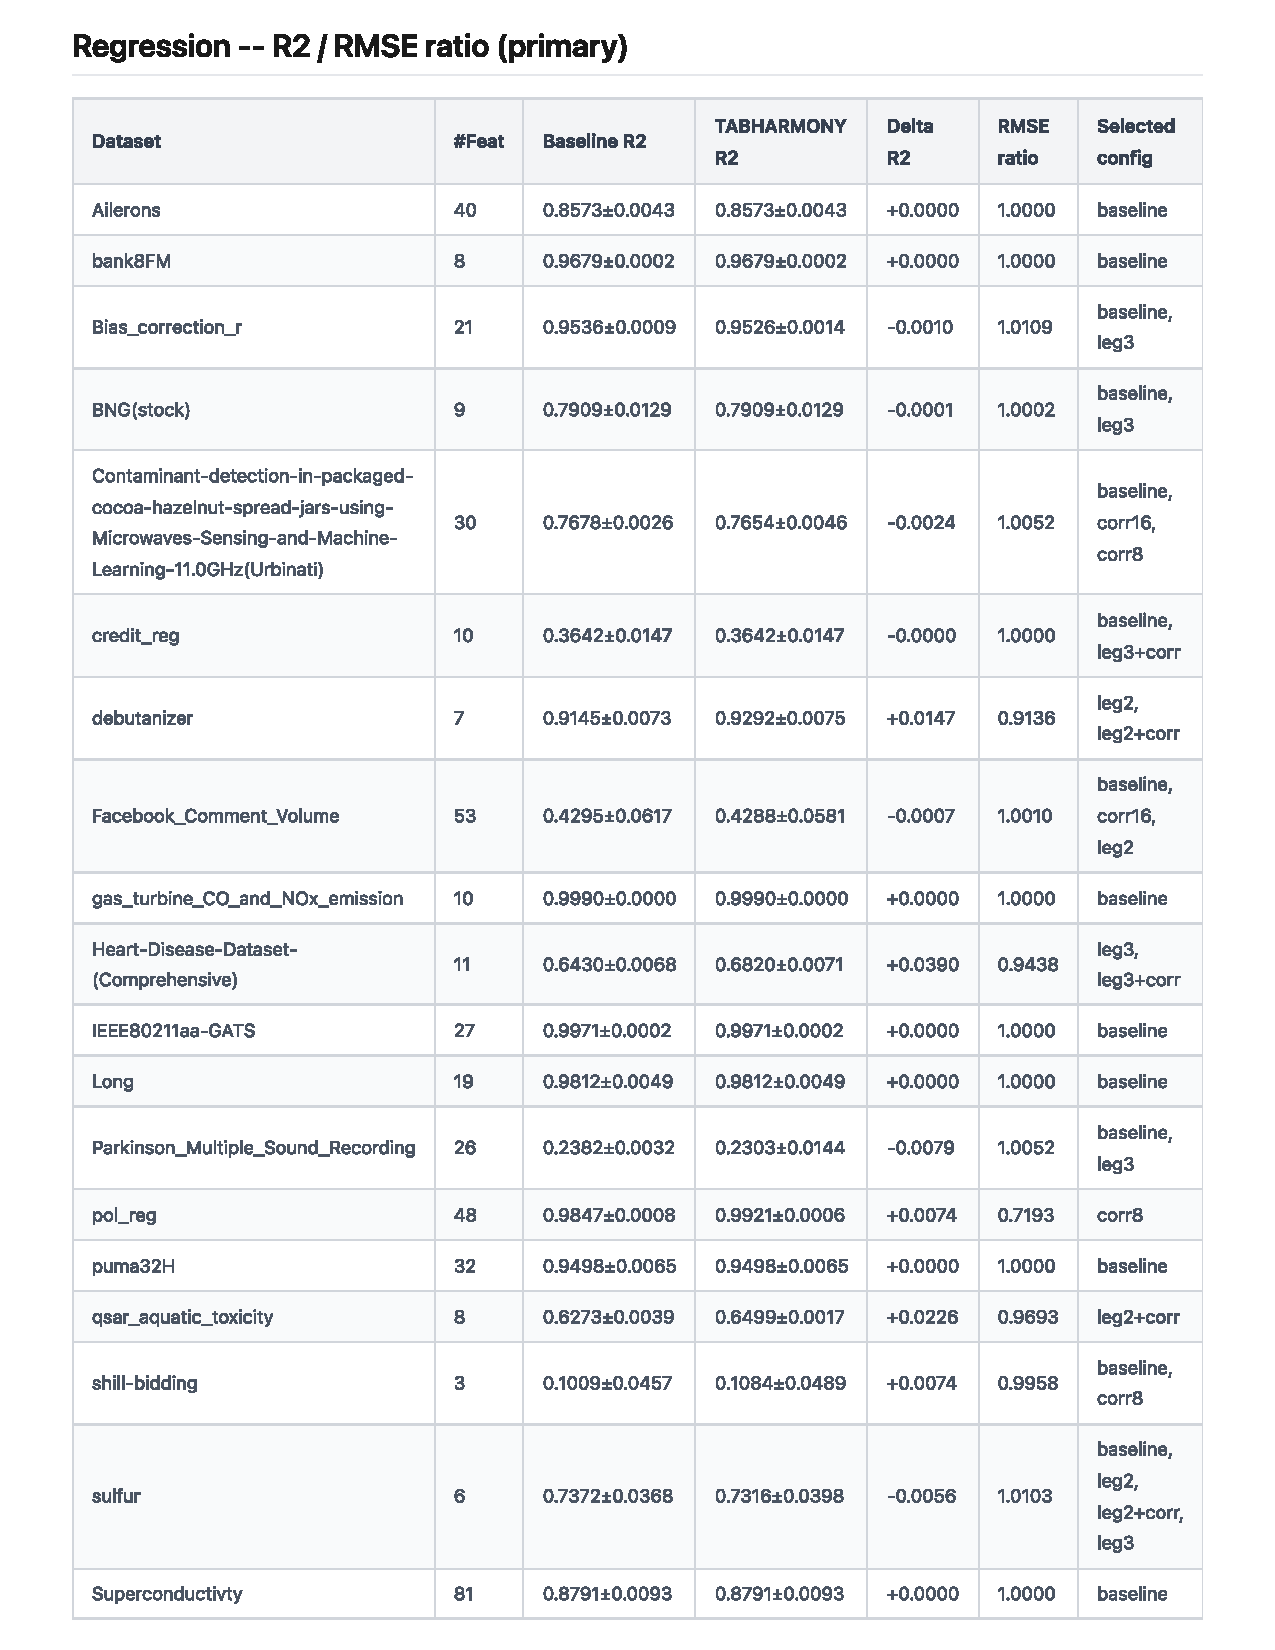
\includegraphics[width=\linewidth]{sections/x_maha_qual/rebuttal_4.pdf}
\end{figure}

\newpage
\begin{figure}[t!]
    \centering
    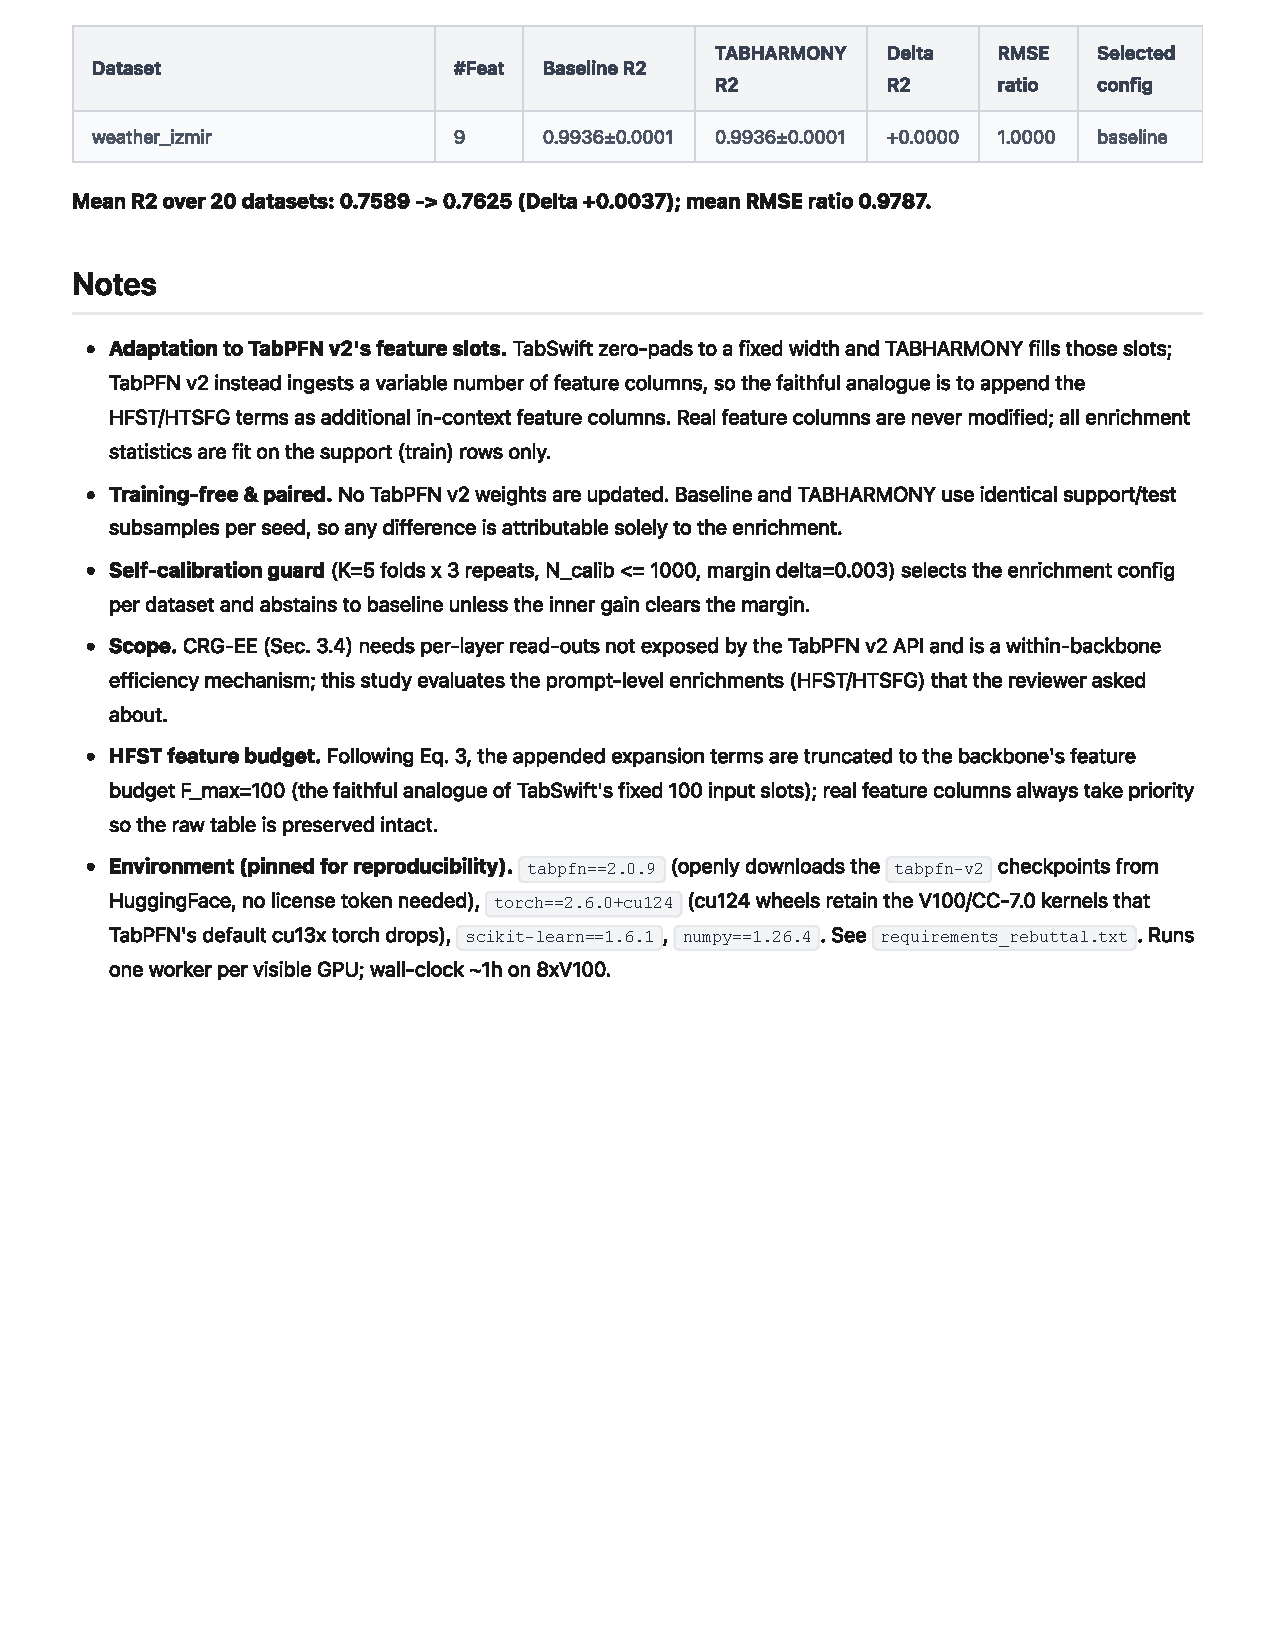
\includegraphics[width=\linewidth]{sections/x_maha_qual/rebuttal_5.pdf}
\end{figure}

\begin{figure}[t!]
    \centering
    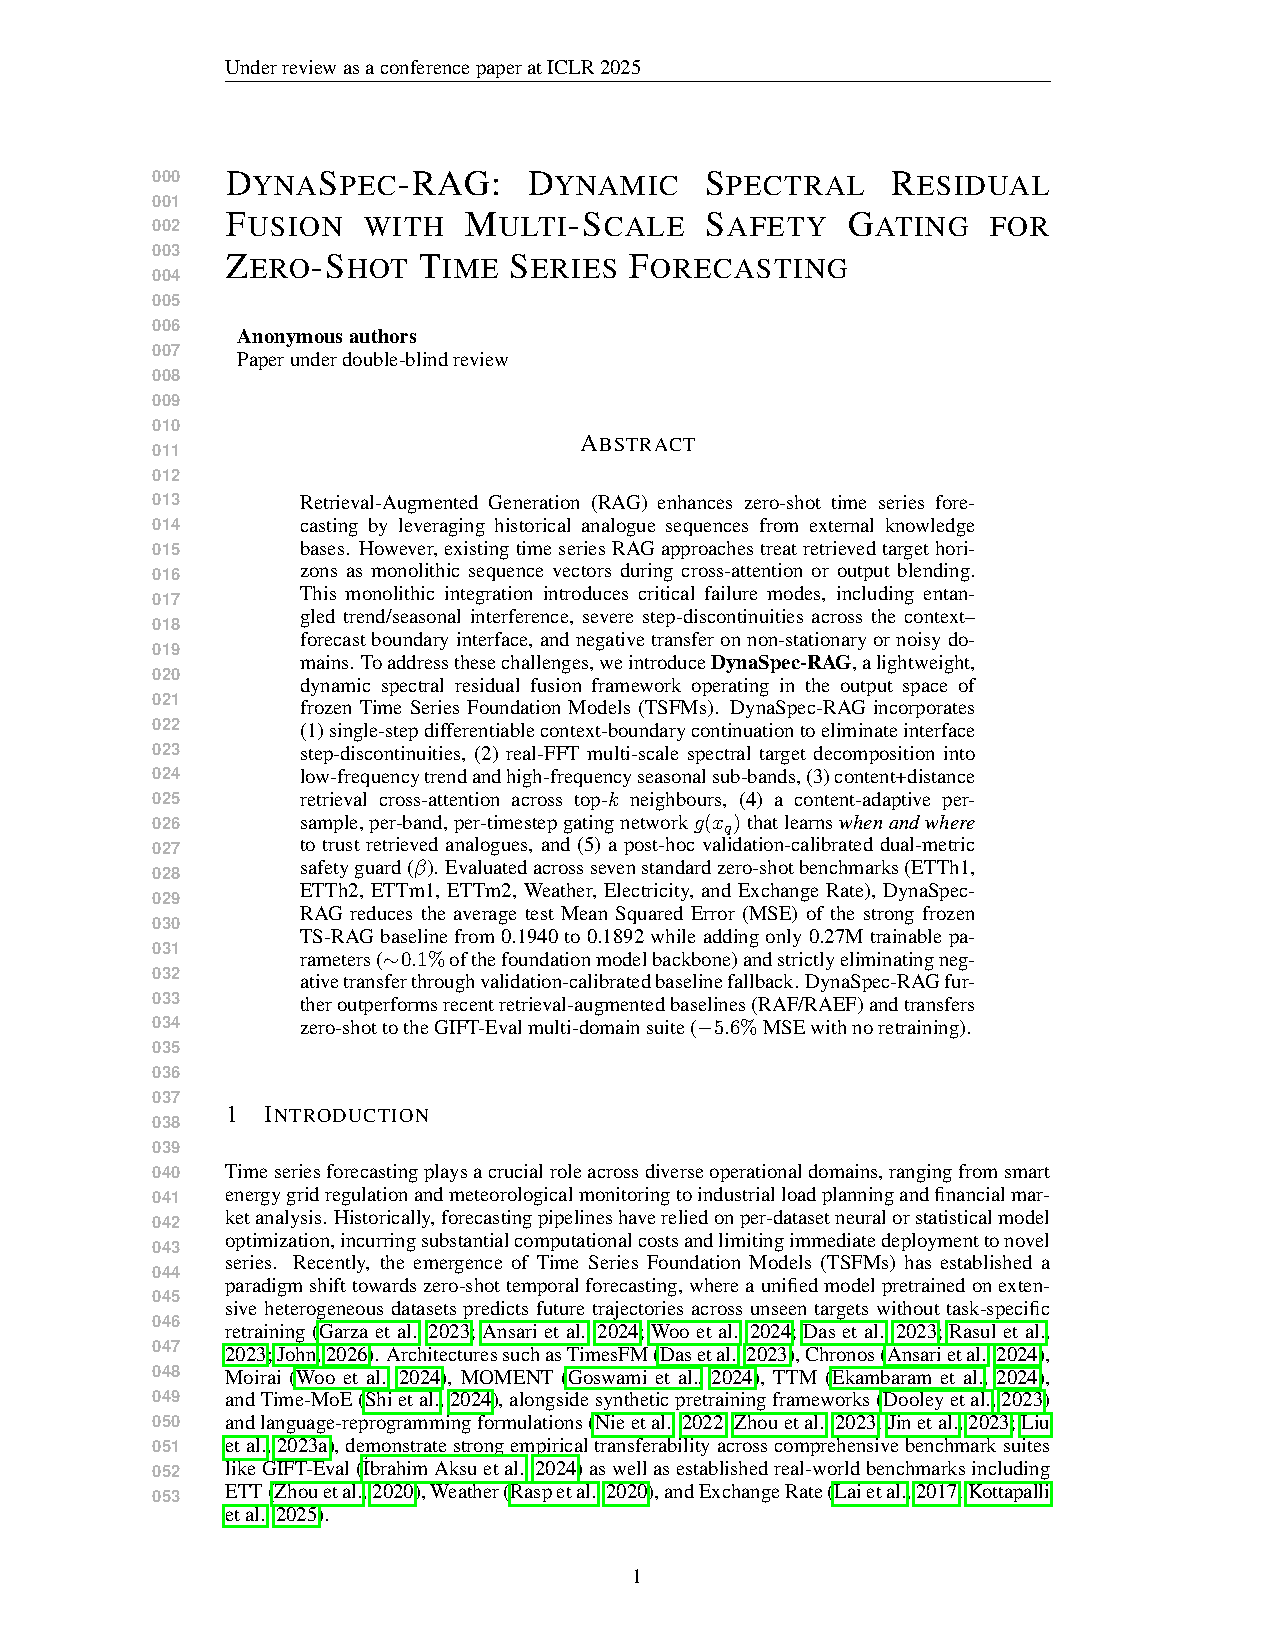
\includegraphics[width=\linewidth]{sections/dynaspec_qual/ts_rag1.pdf}
\end{figure}

\begin{figure}[t!]
    \centering
    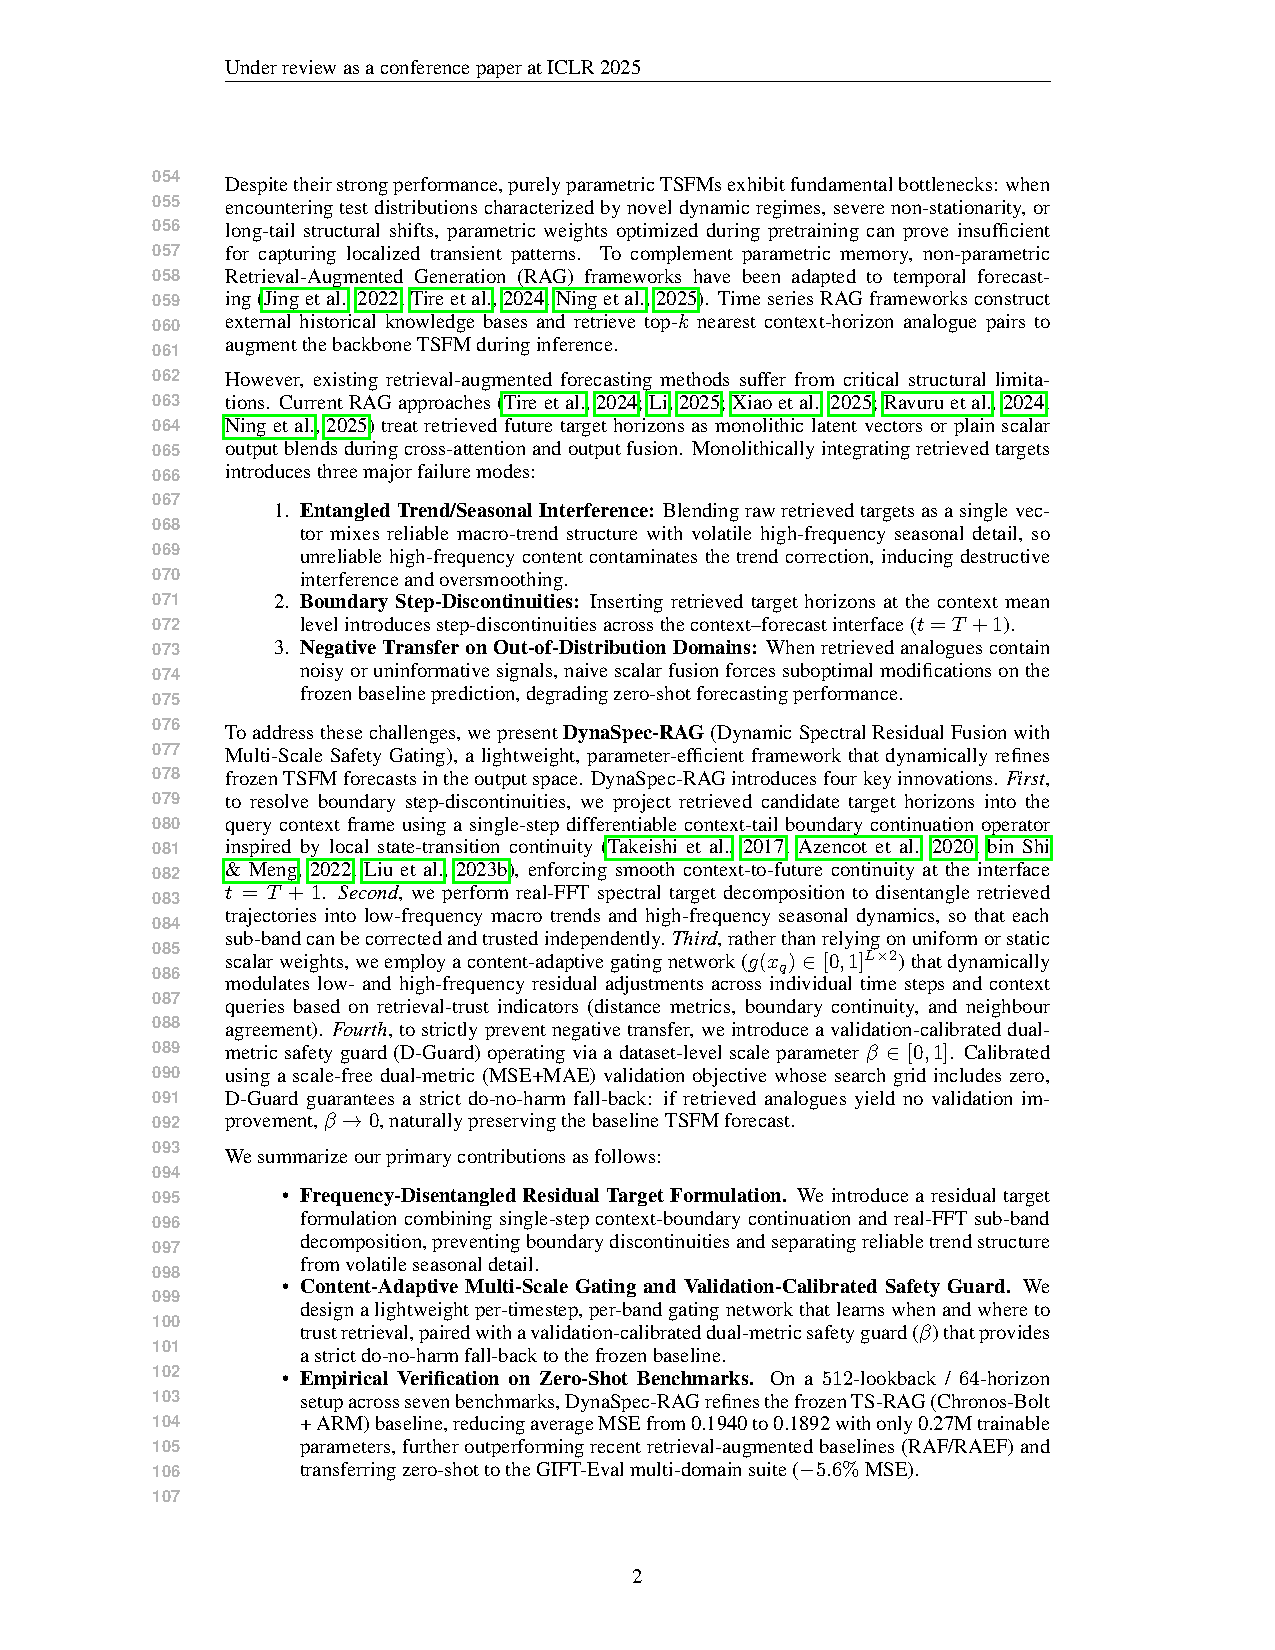
\includegraphics[width=\linewidth]{sections/dynaspec_qual/ts_rag2.pdf}
\end{figure}

\begin{figure}[t!]
    \centering
    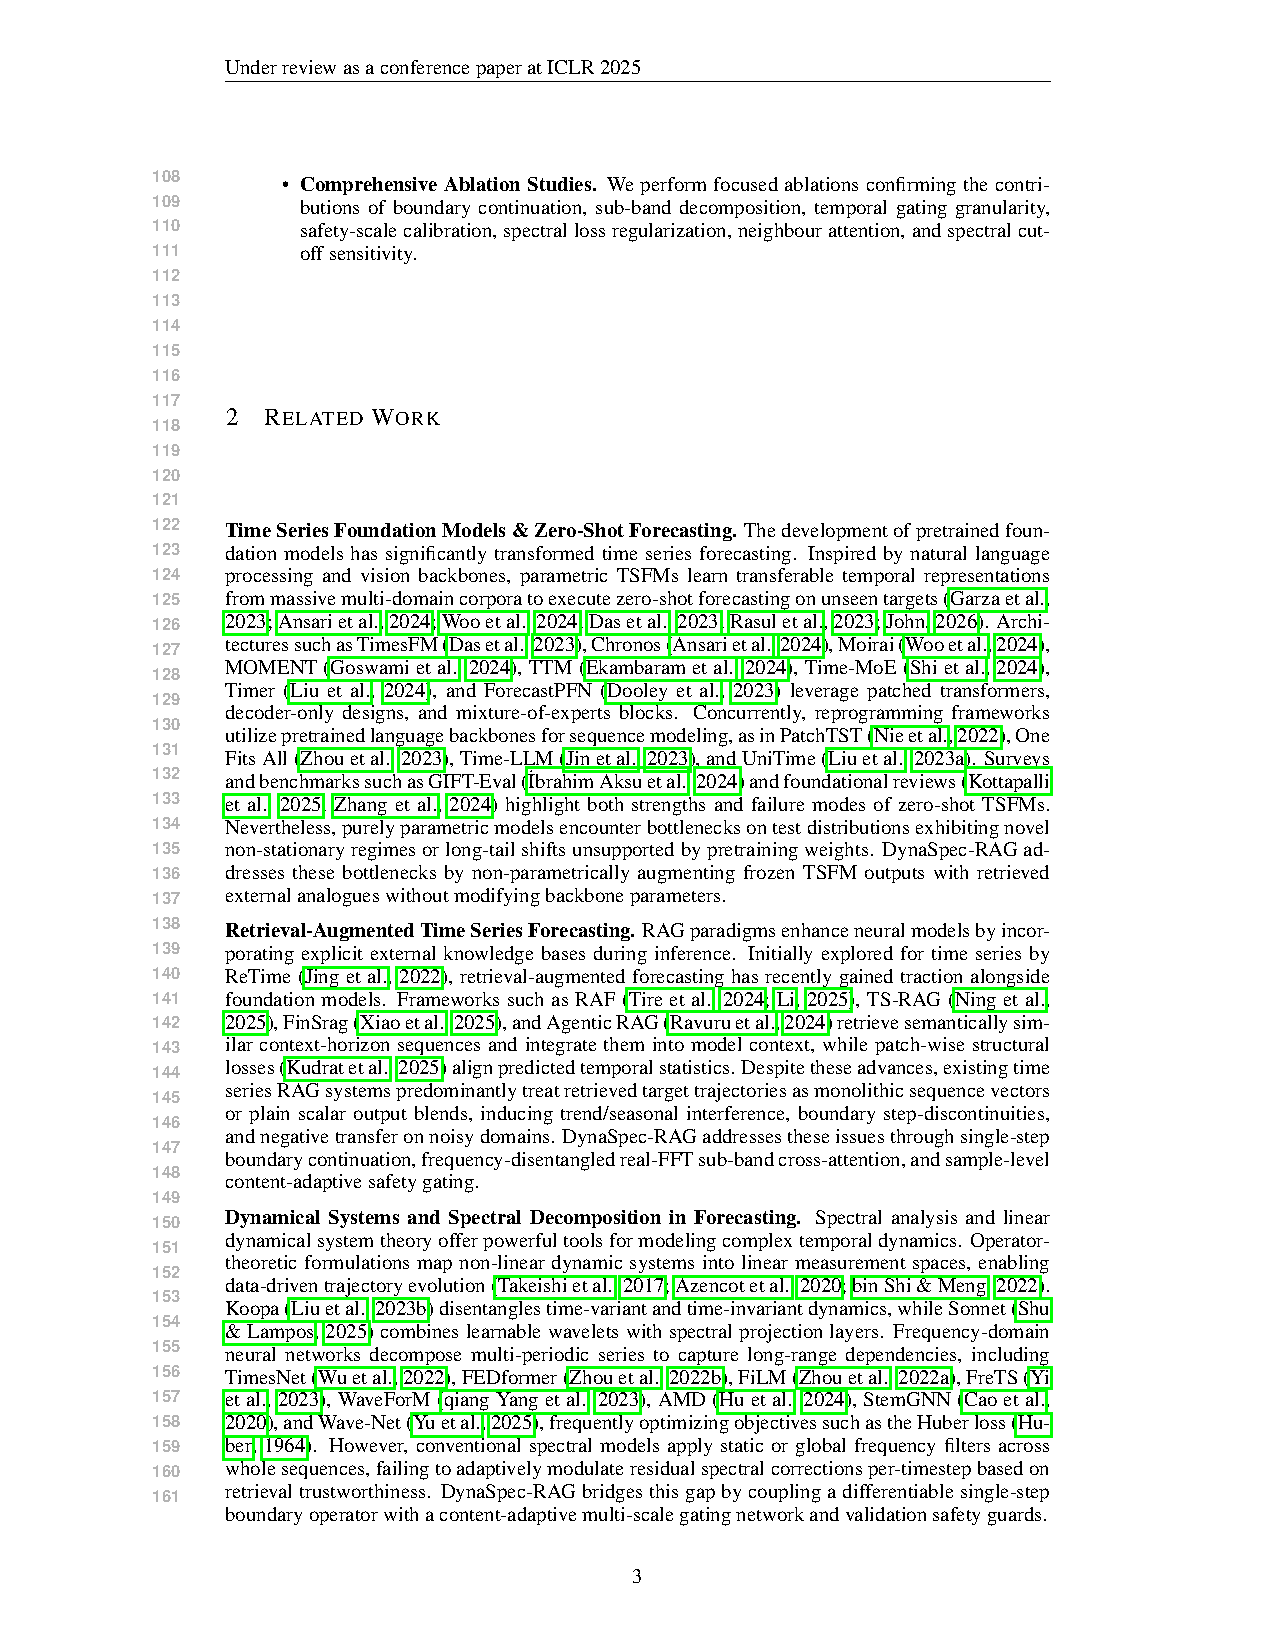
\includegraphics[width=\linewidth]{sections/dynaspec_qual/ts_rag3.pdf}
\end{figure}

\begin{figure}[t!]
    \centering
    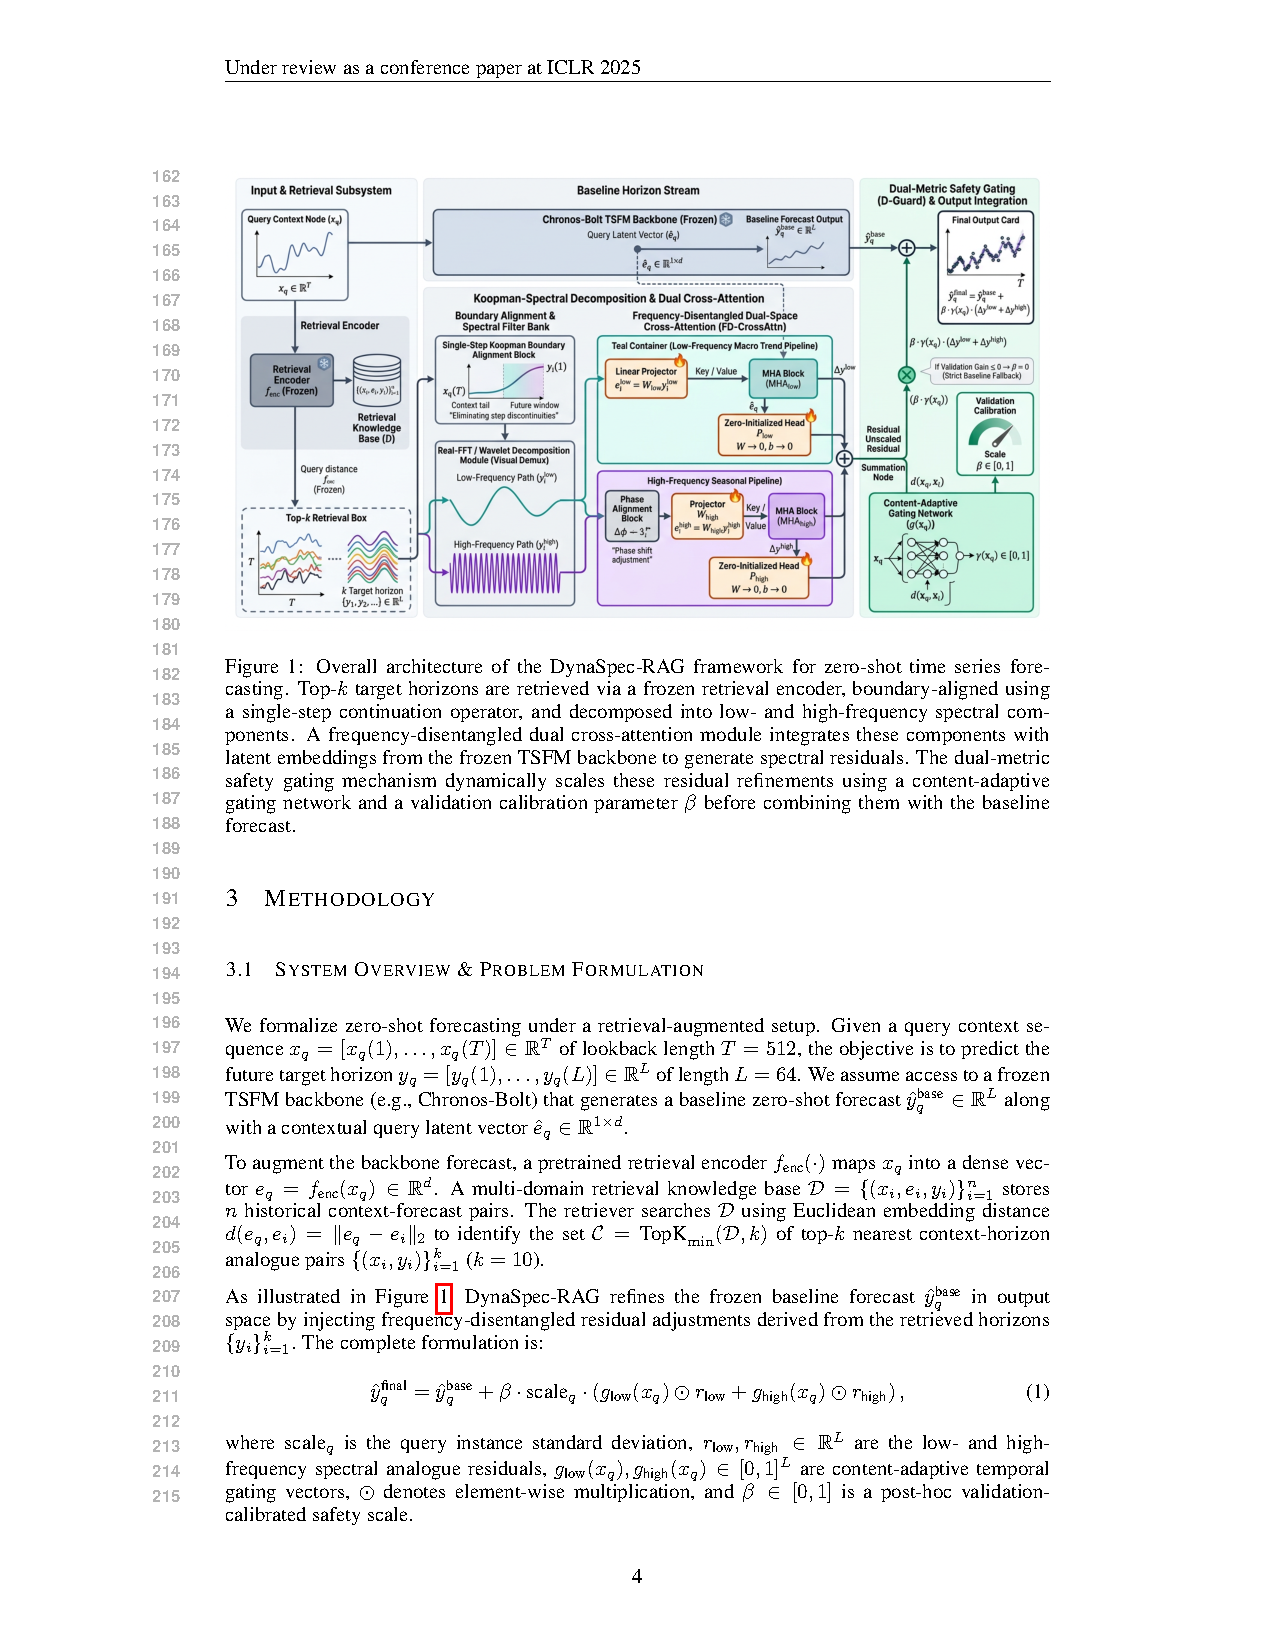
\includegraphics[width=\linewidth]{sections/dynaspec_qual/ts_rag4.pdf}
\end{figure}

\begin{figure}[t!]
    \centering
    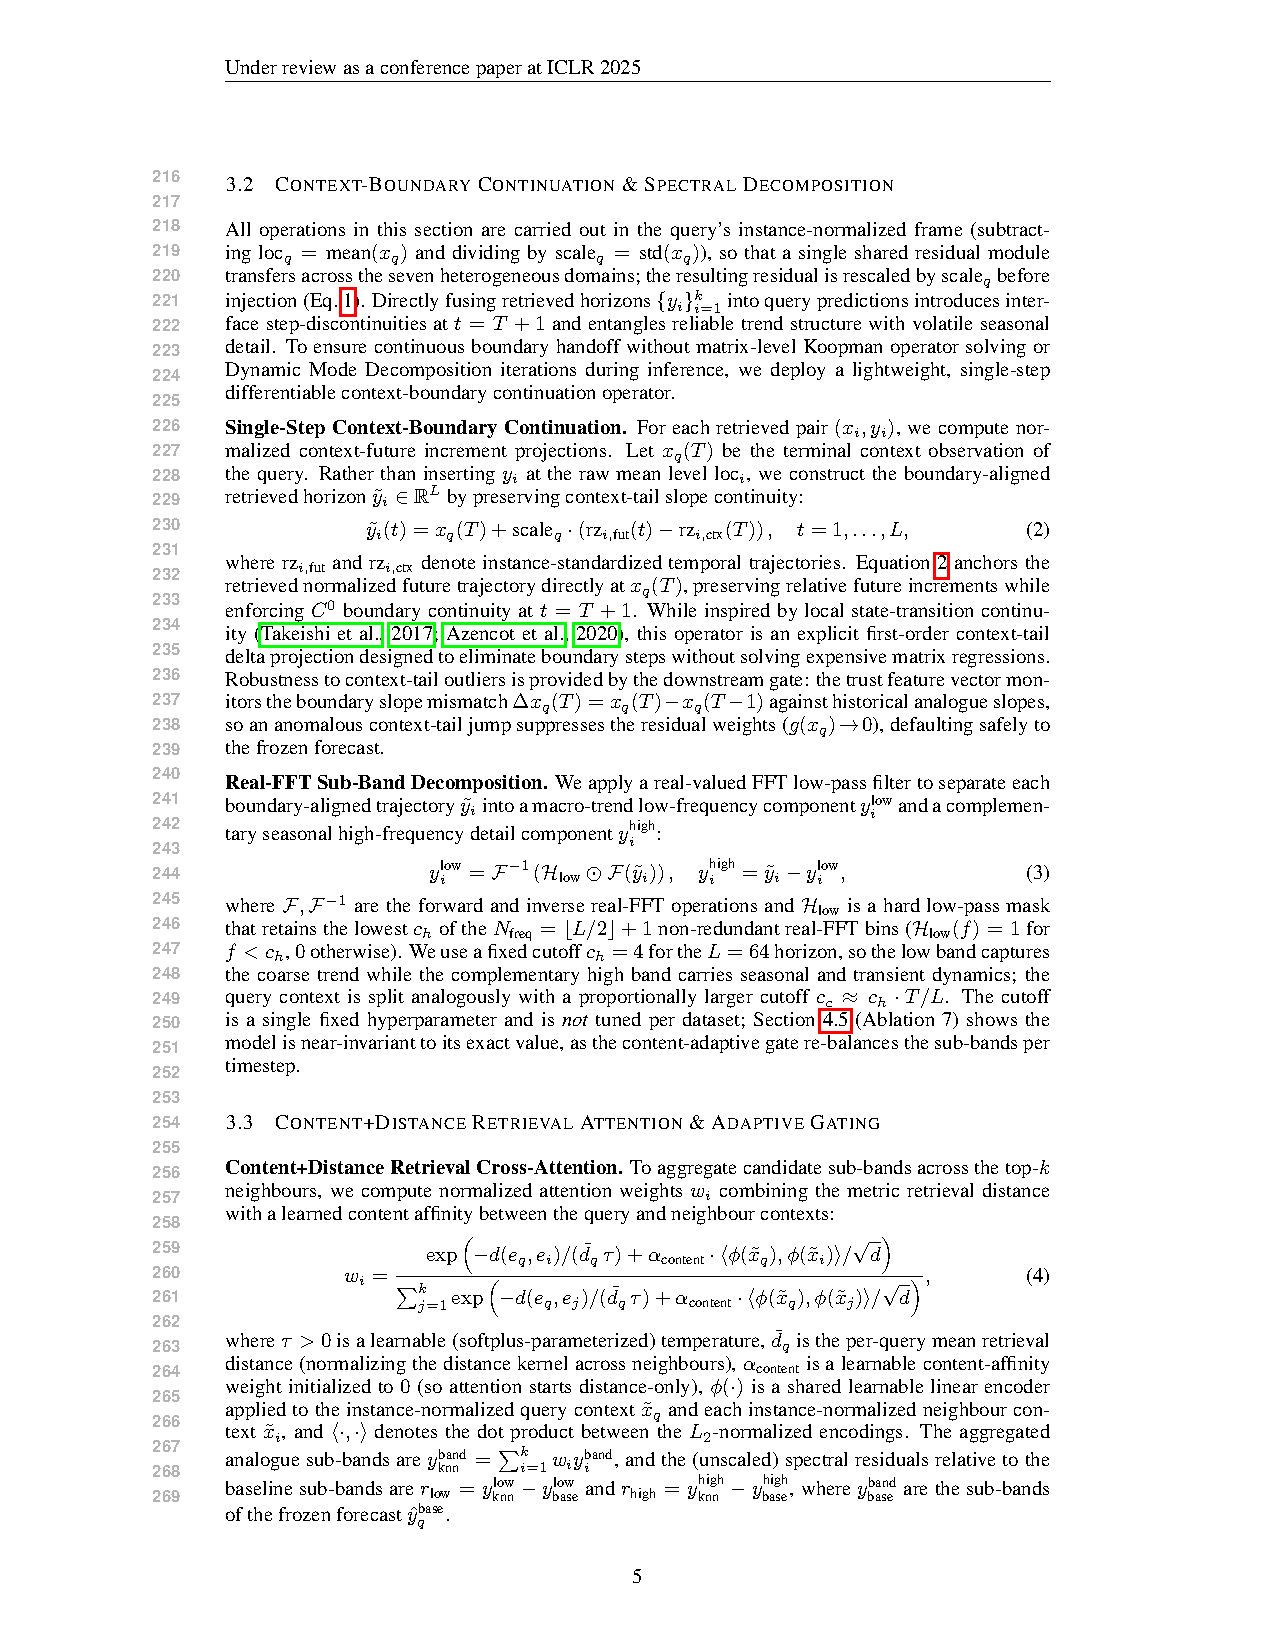
\includegraphics[width=\linewidth]{sections/dynaspec_qual/ts_rag5.pdf}
\end{figure}

\begin{figure}[t!]
    \centering
    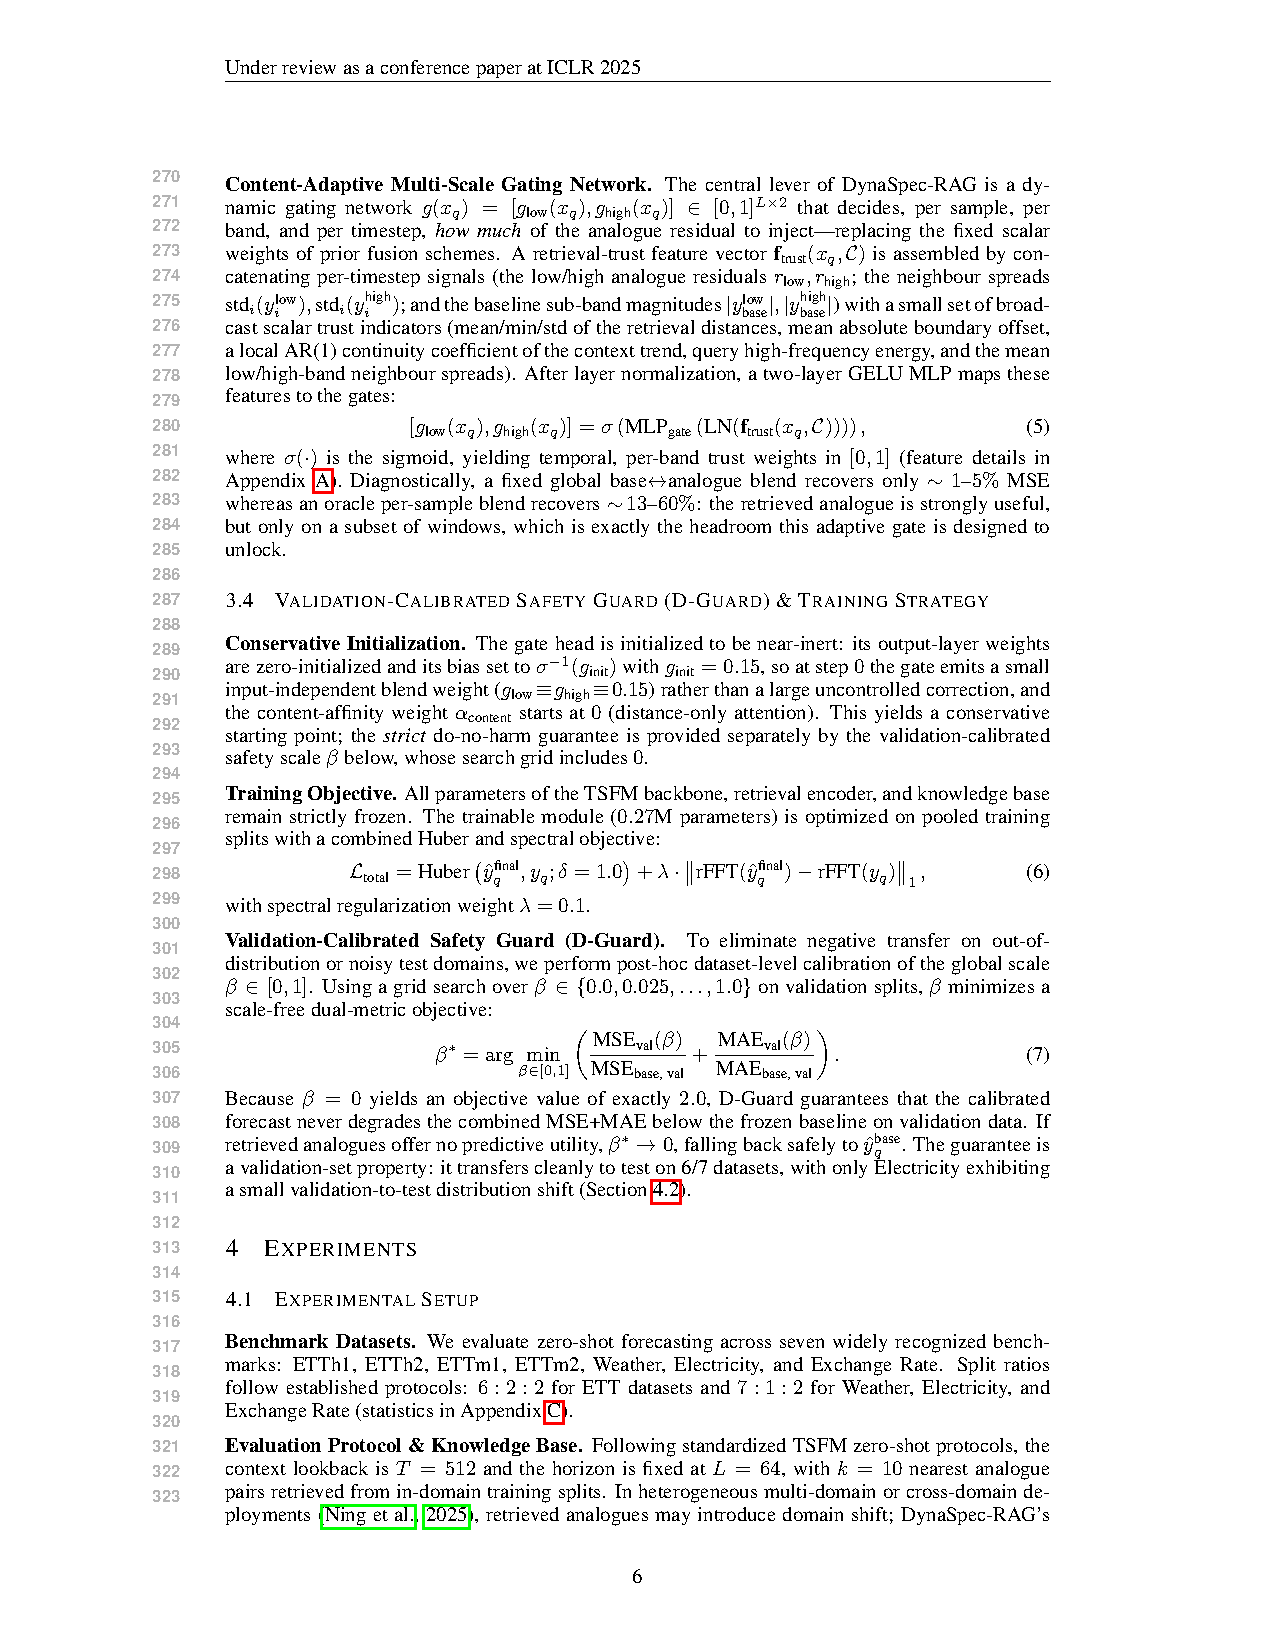
\includegraphics[width=\linewidth]{sections/dynaspec_qual/ts_rag6.pdf}
\end{figure}

\begin{figure}[t!]
    \centering
    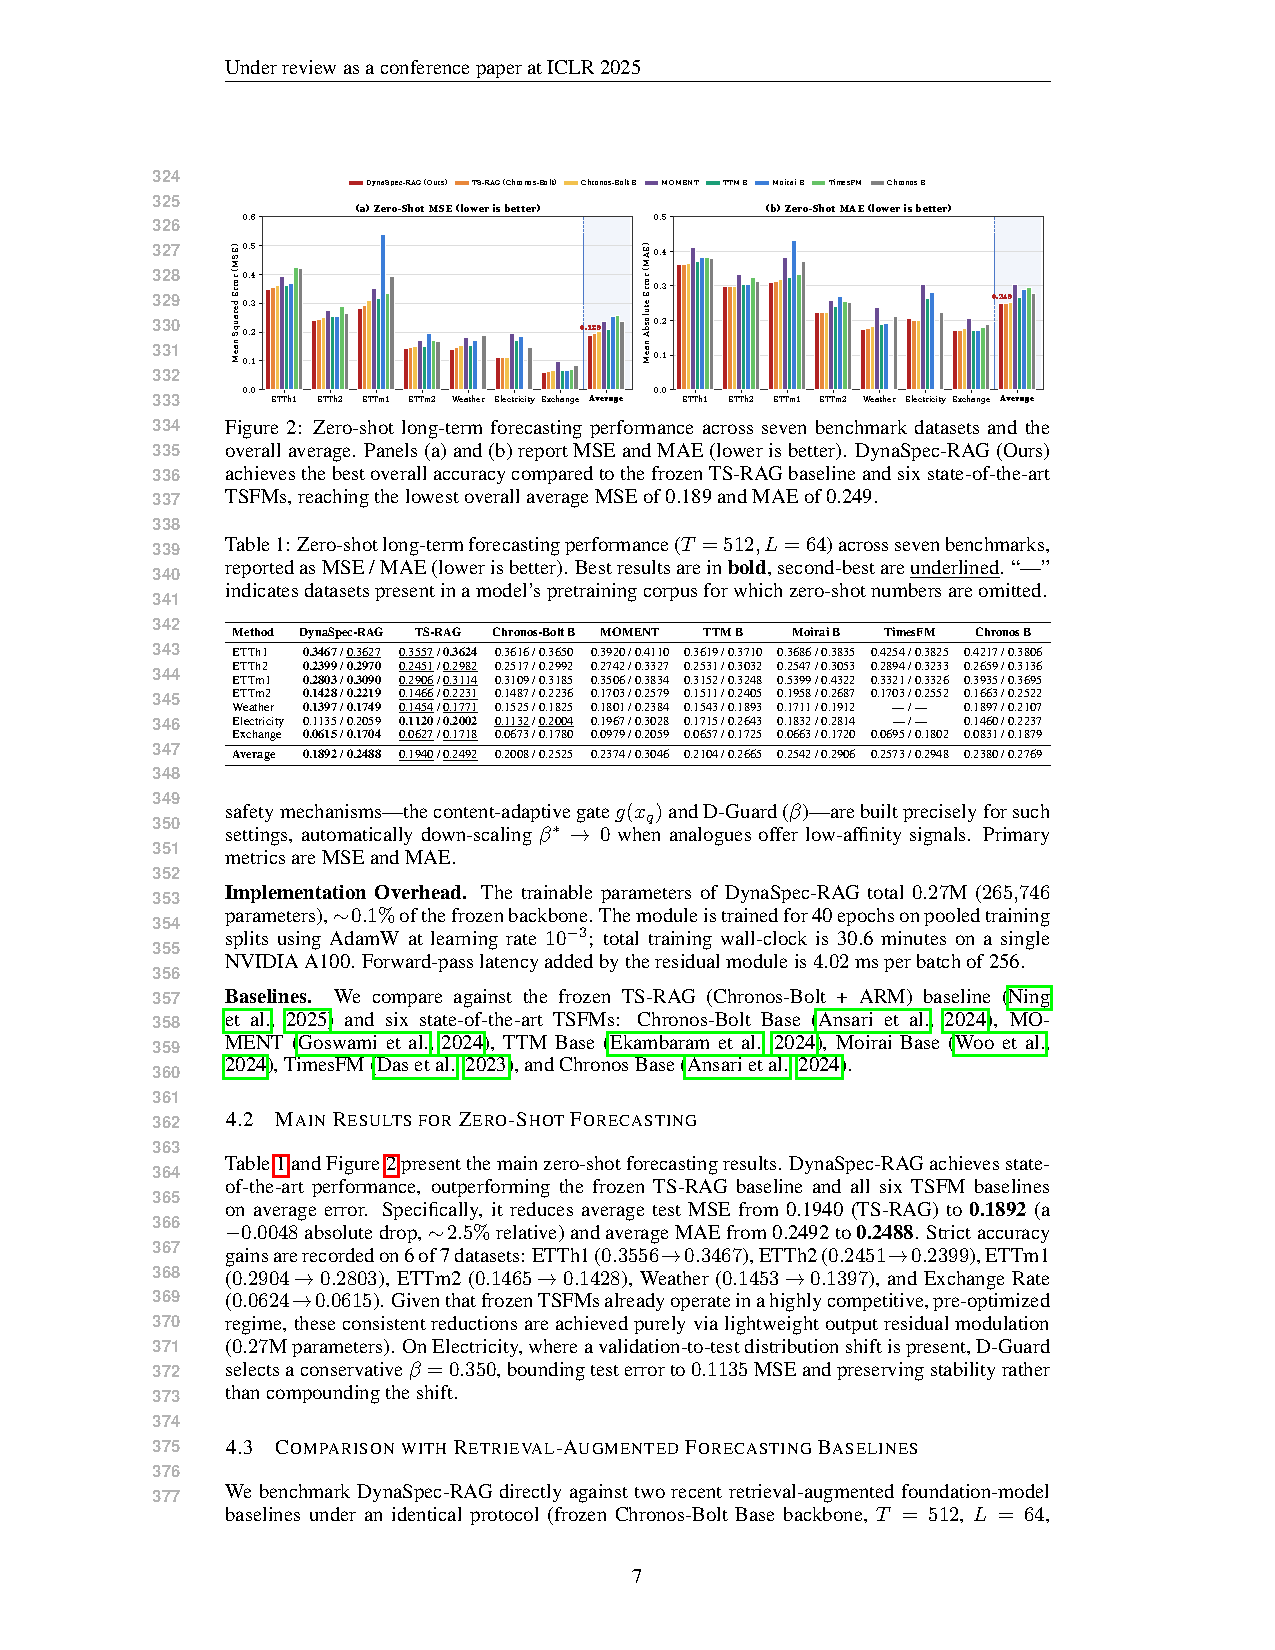
\includegraphics[width=\linewidth]{sections/dynaspec_qual/ts_rag7.pdf}
\end{figure}

\begin{figure}[t!]
    \centering
    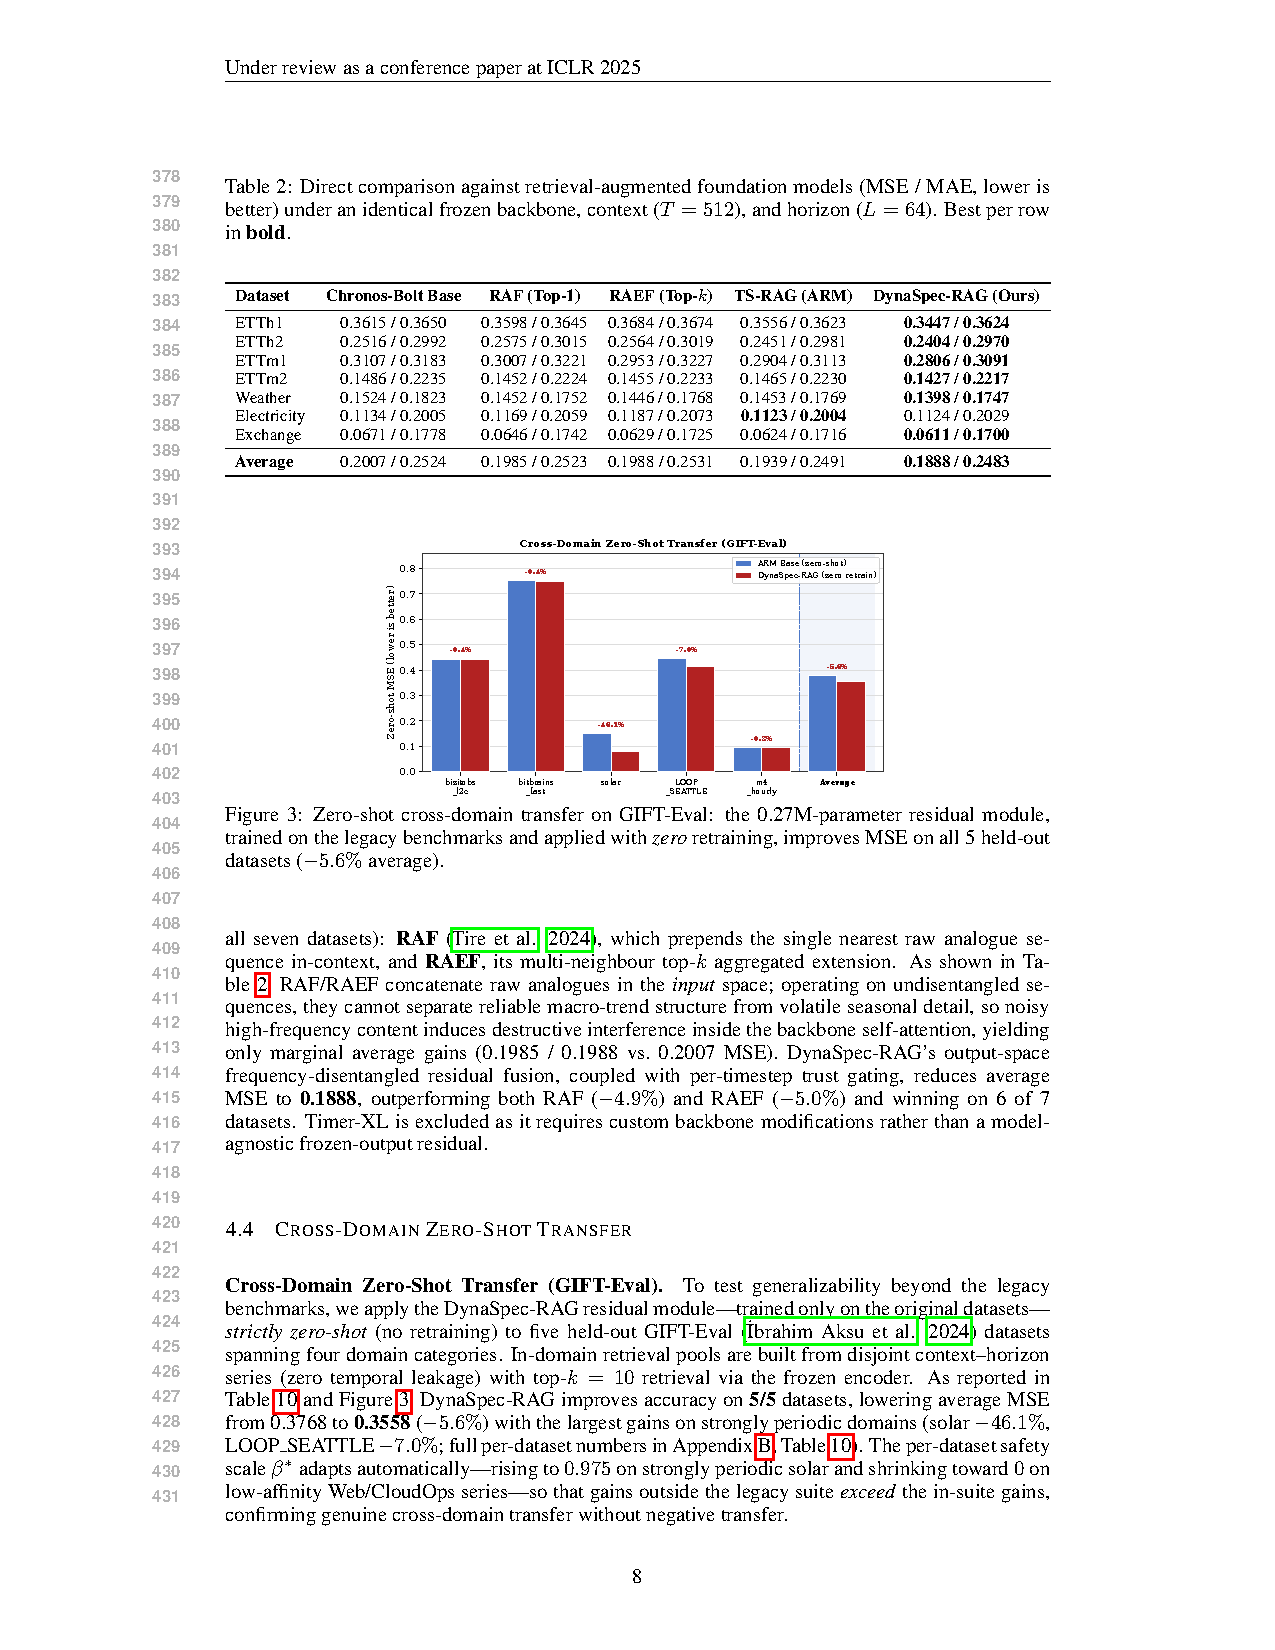
\includegraphics[width=\linewidth]{sections/dynaspec_qual/ts_rag8.pdf}
\end{figure}

\begin{figure}[t!]
    \centering
    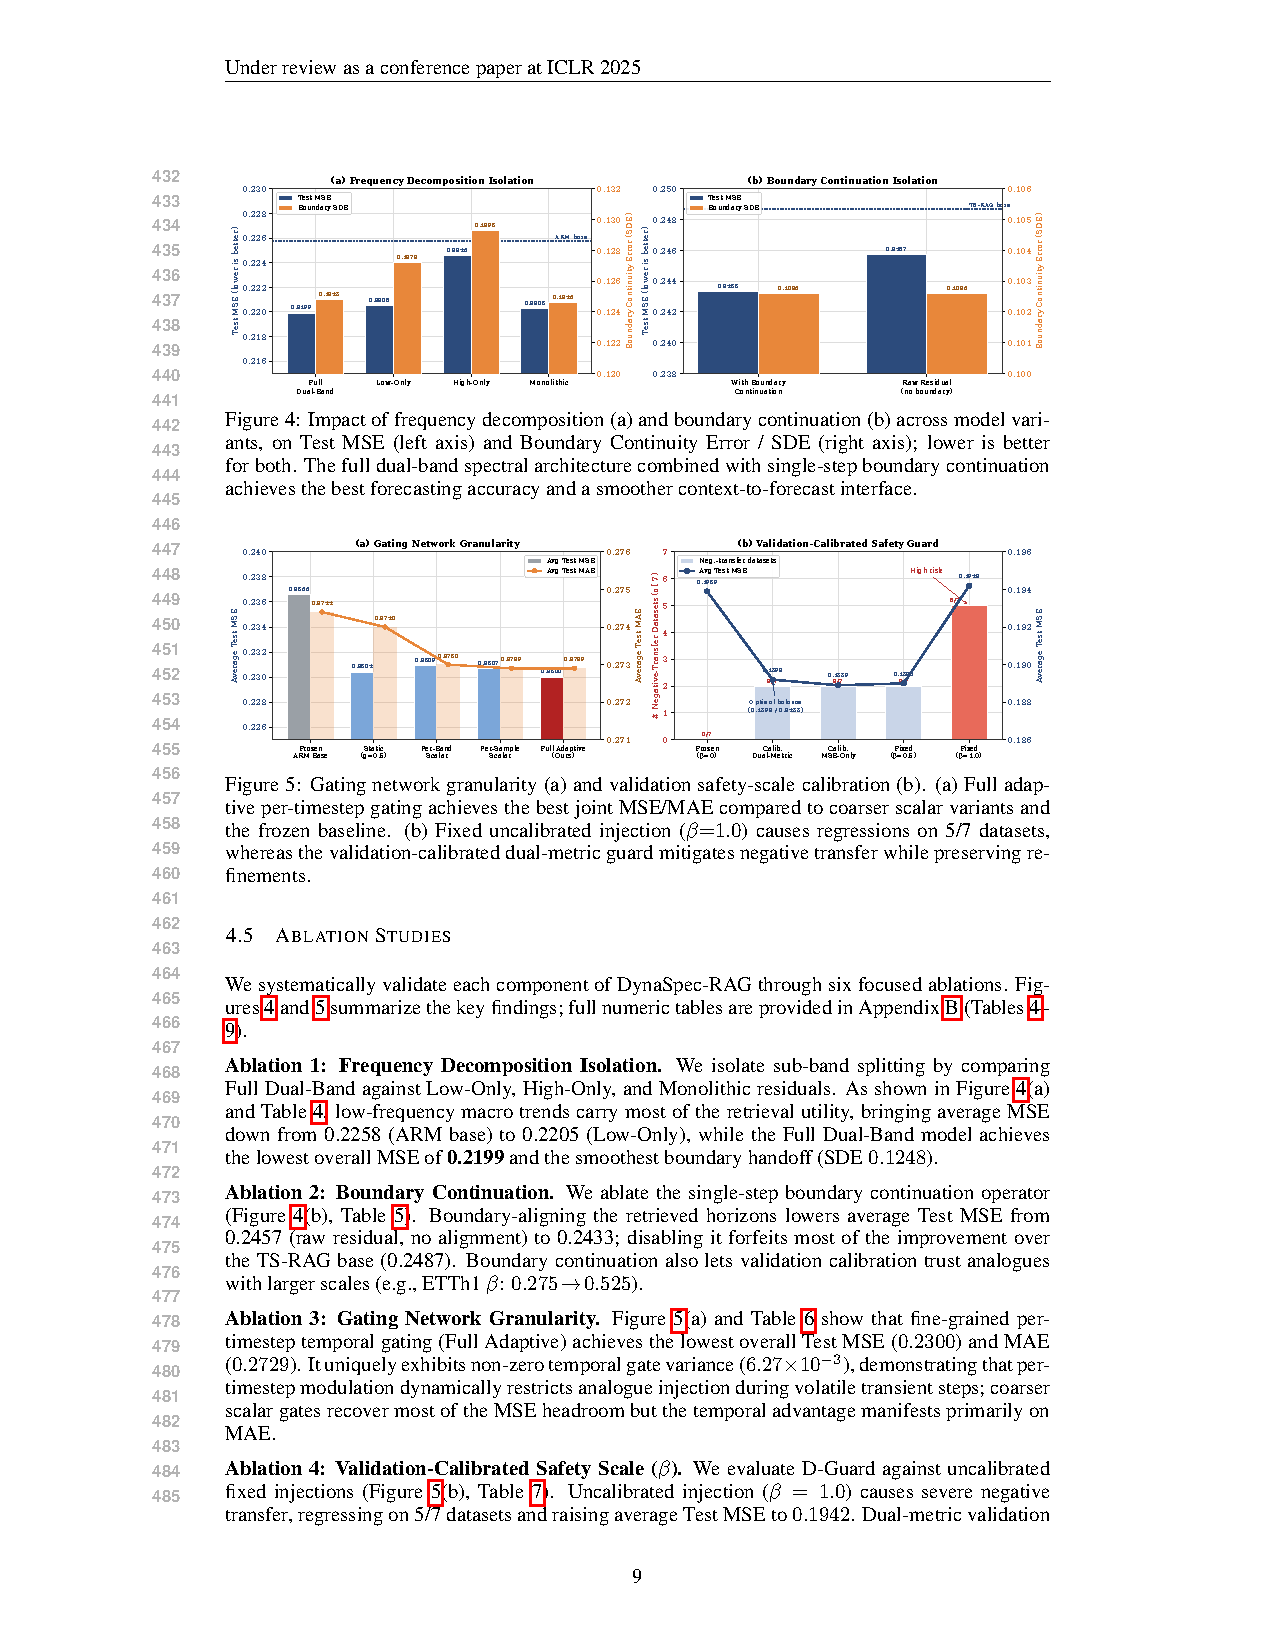
\includegraphics[width=\linewidth]{sections/dynaspec_qual/ts_rag9.pdf}
\end{figure}

\begin{figure}[t!]
    \centering
    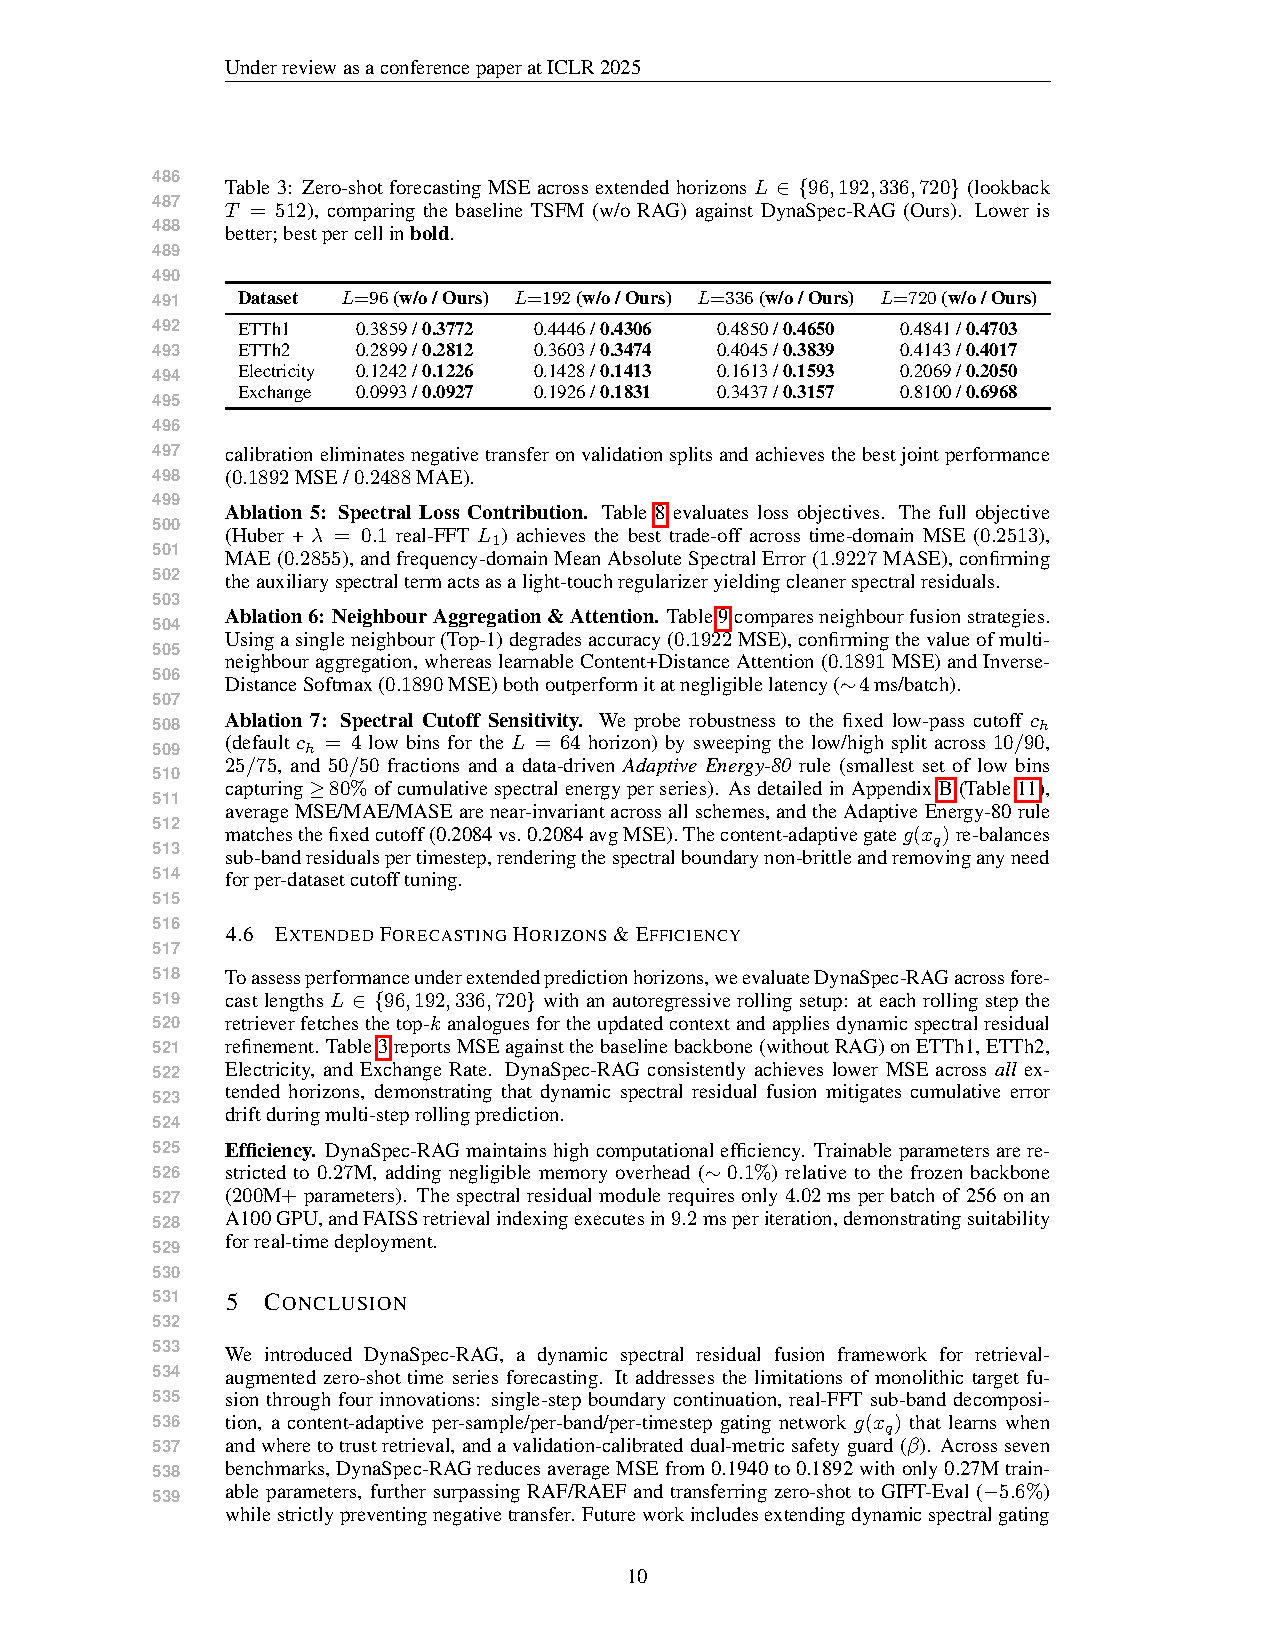
\includegraphics[width=\linewidth]{sections/dynaspec_qual/ts_rag10.pdf}
\end{figure}

\begin{figure}[t!]
    \centering
    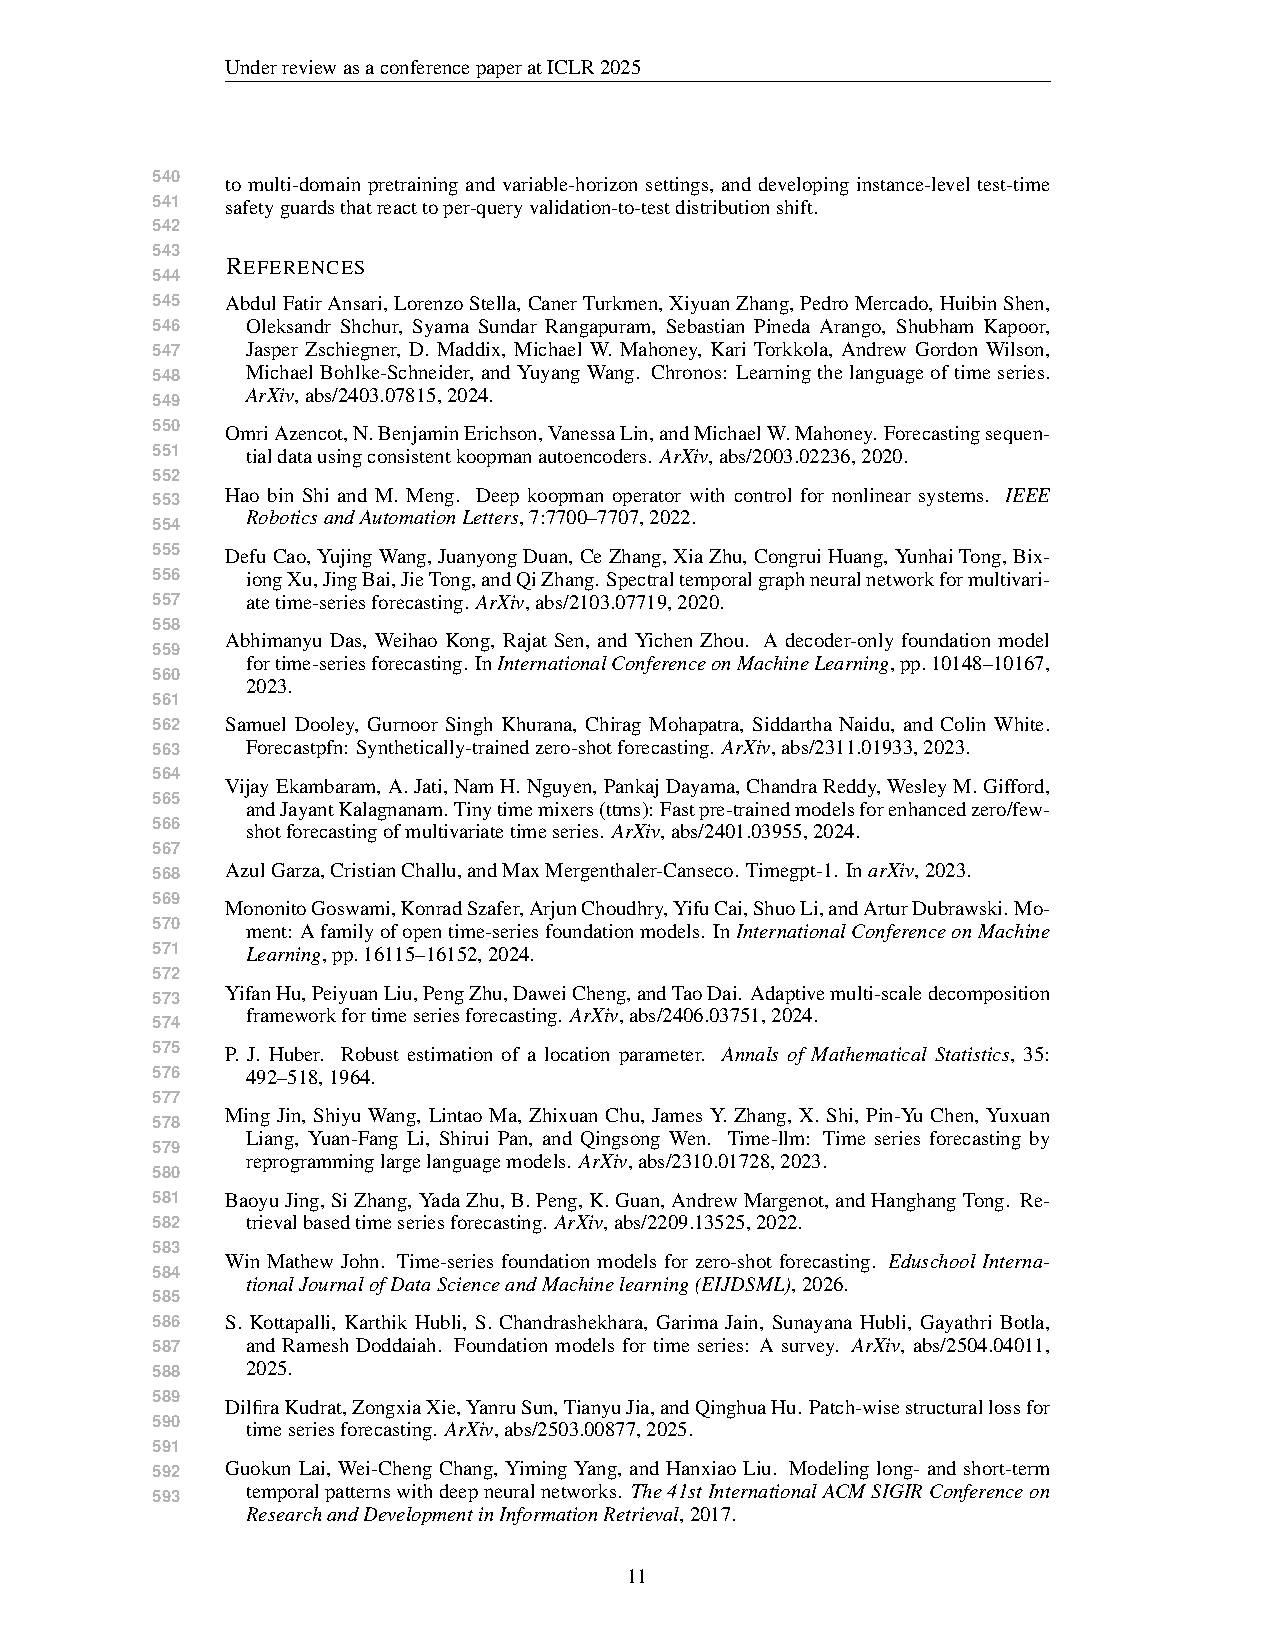
\includegraphics[width=\linewidth]{sections/dynaspec_qual/ts_rag11.pdf}
\end{figure}

\begin{figure}[t!]
    \centering
    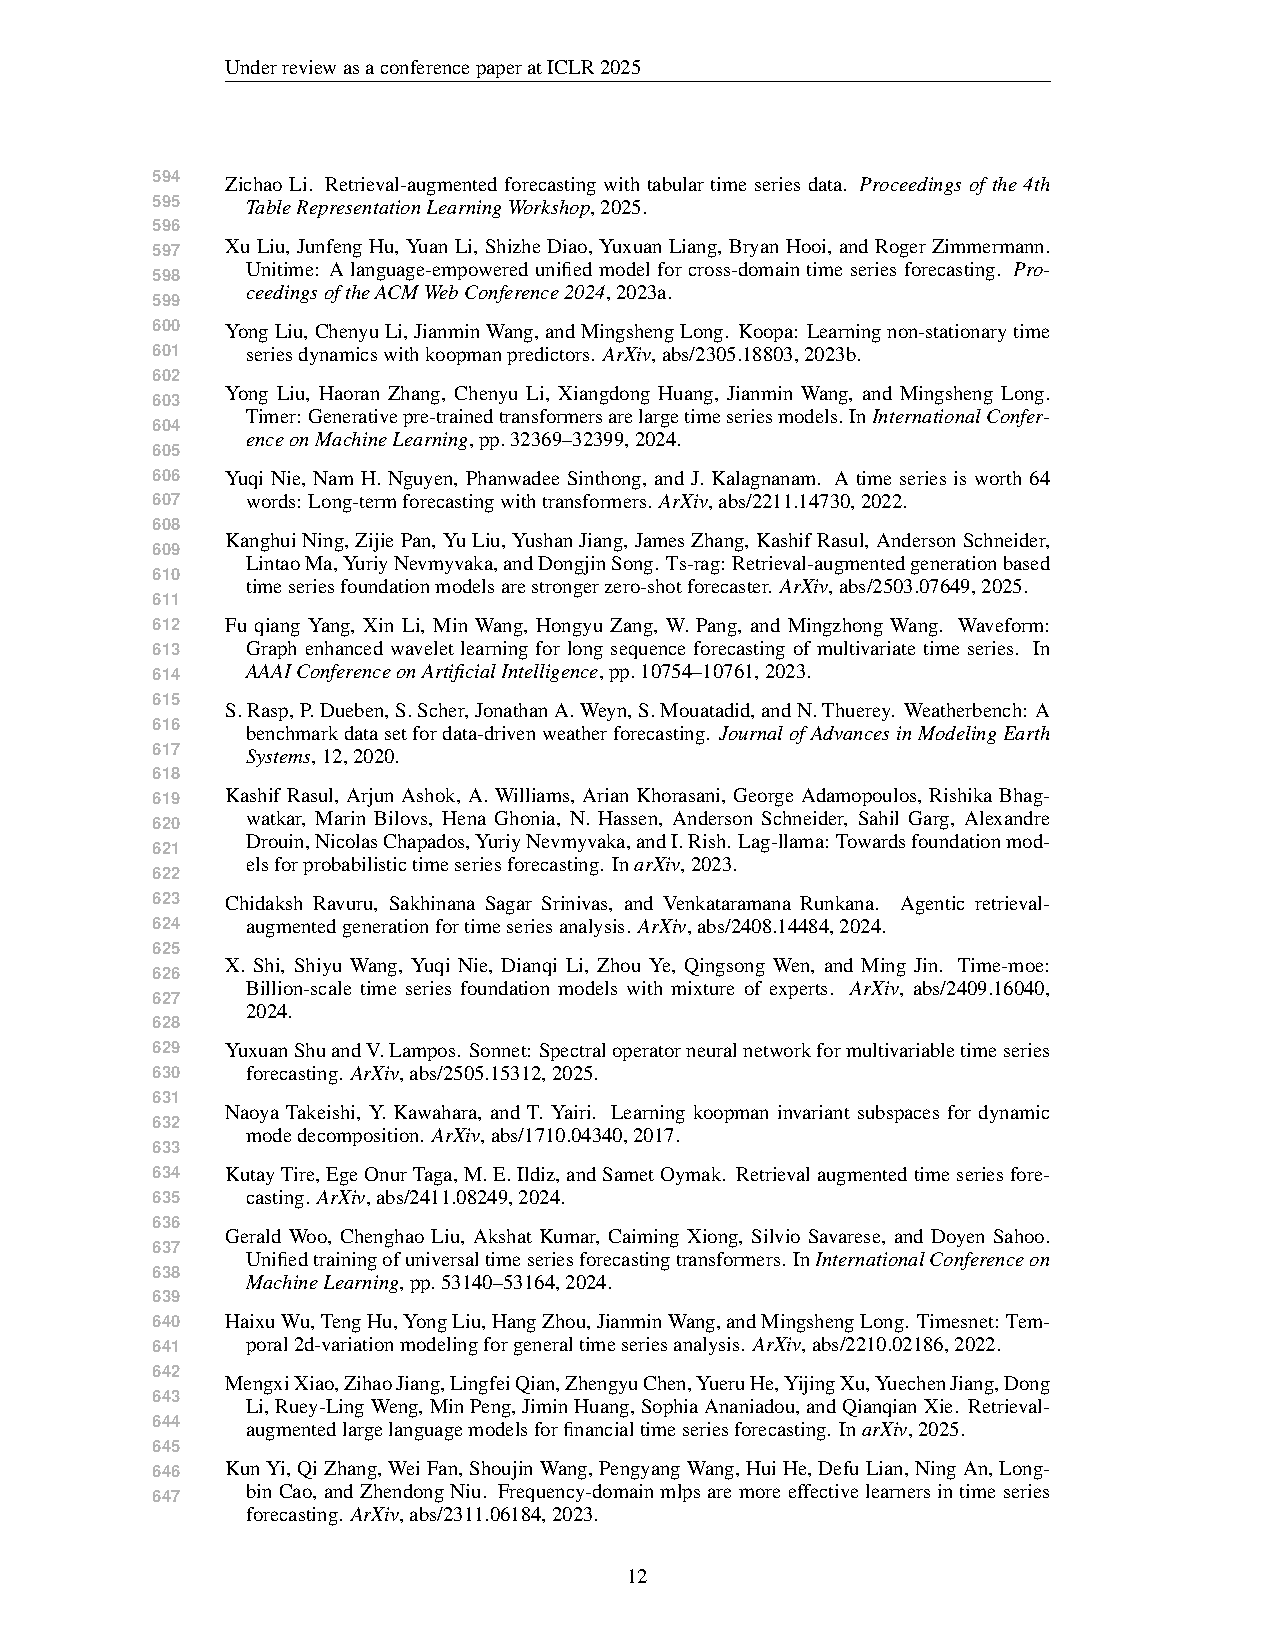
\includegraphics[width=\linewidth]{sections/dynaspec_qual/ts_rag12.pdf}
\end{figure}

\begin{figure}[t!]
    \centering
    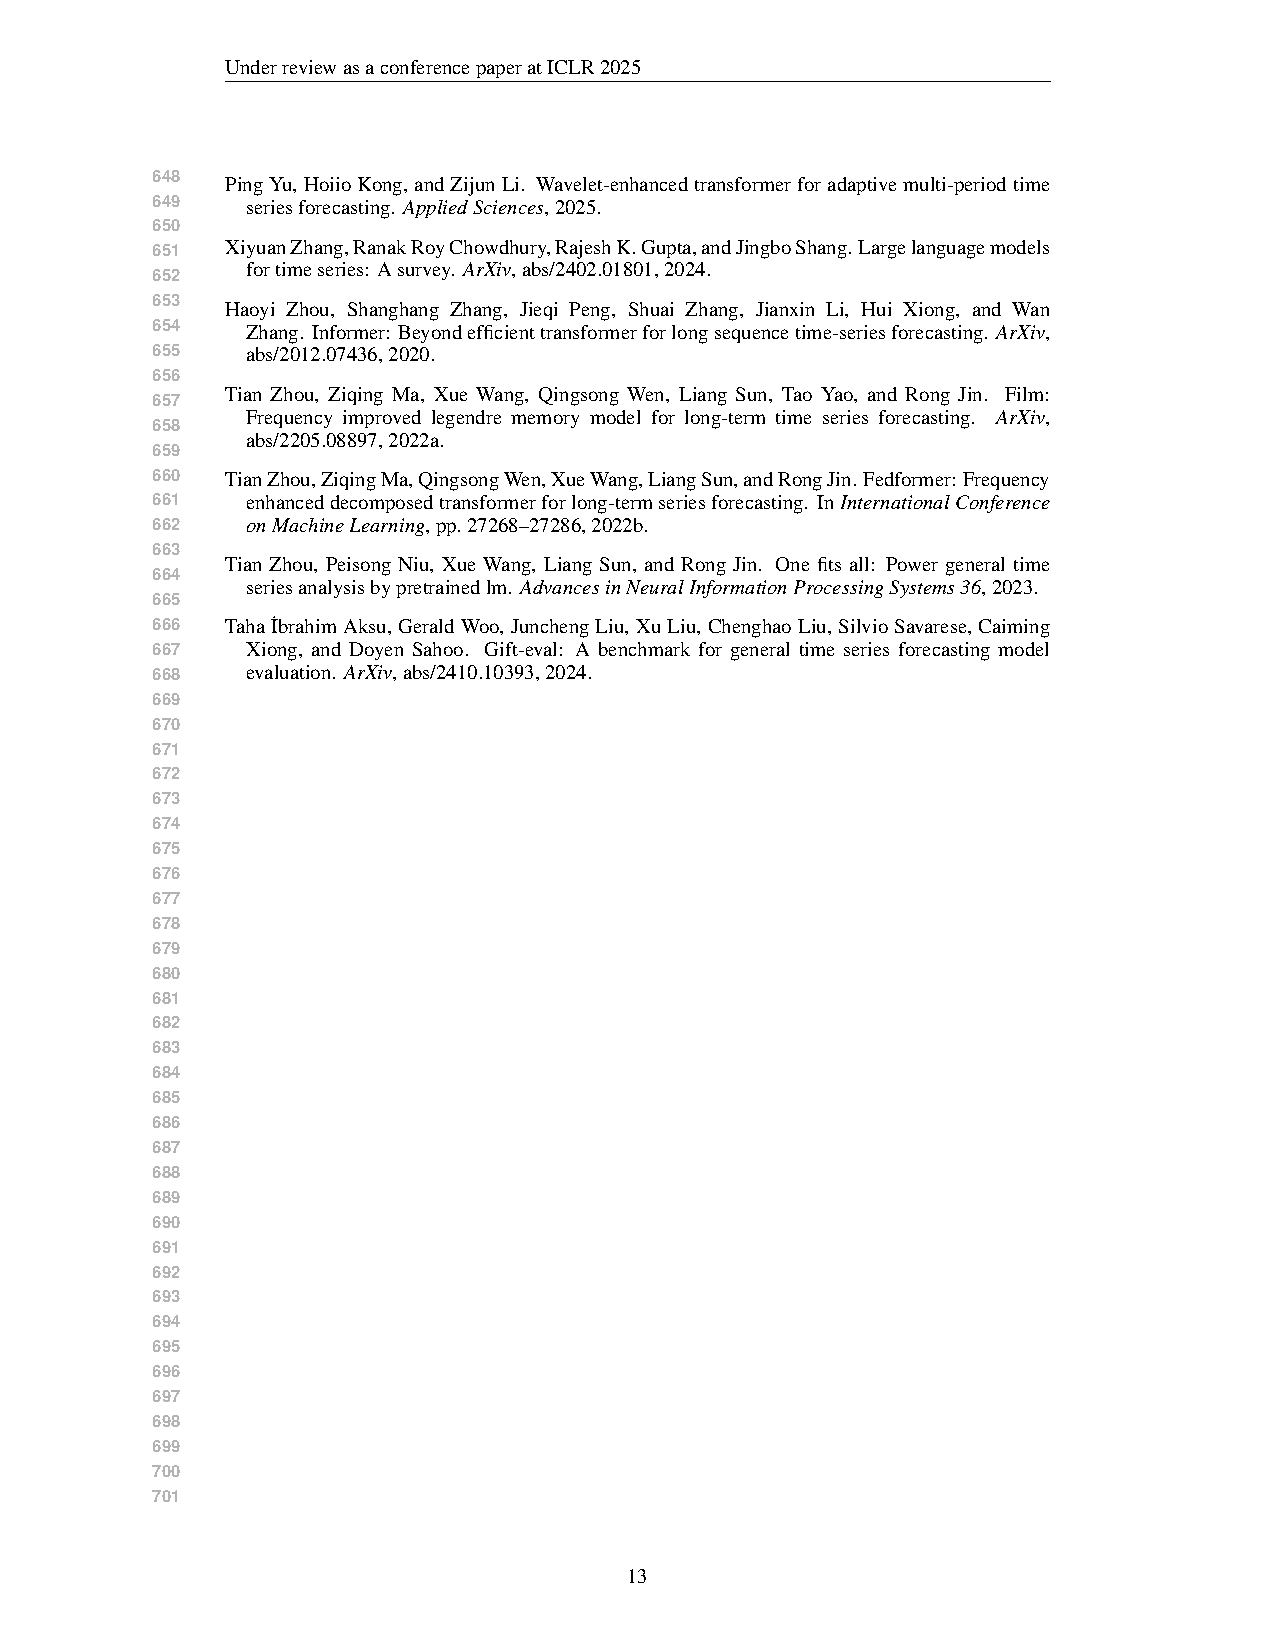
\includegraphics[width=\linewidth]{sections/dynaspec_qual/ts_rag13.pdf}
\end{figure}

\begin{figure}[t!]
    \centering
    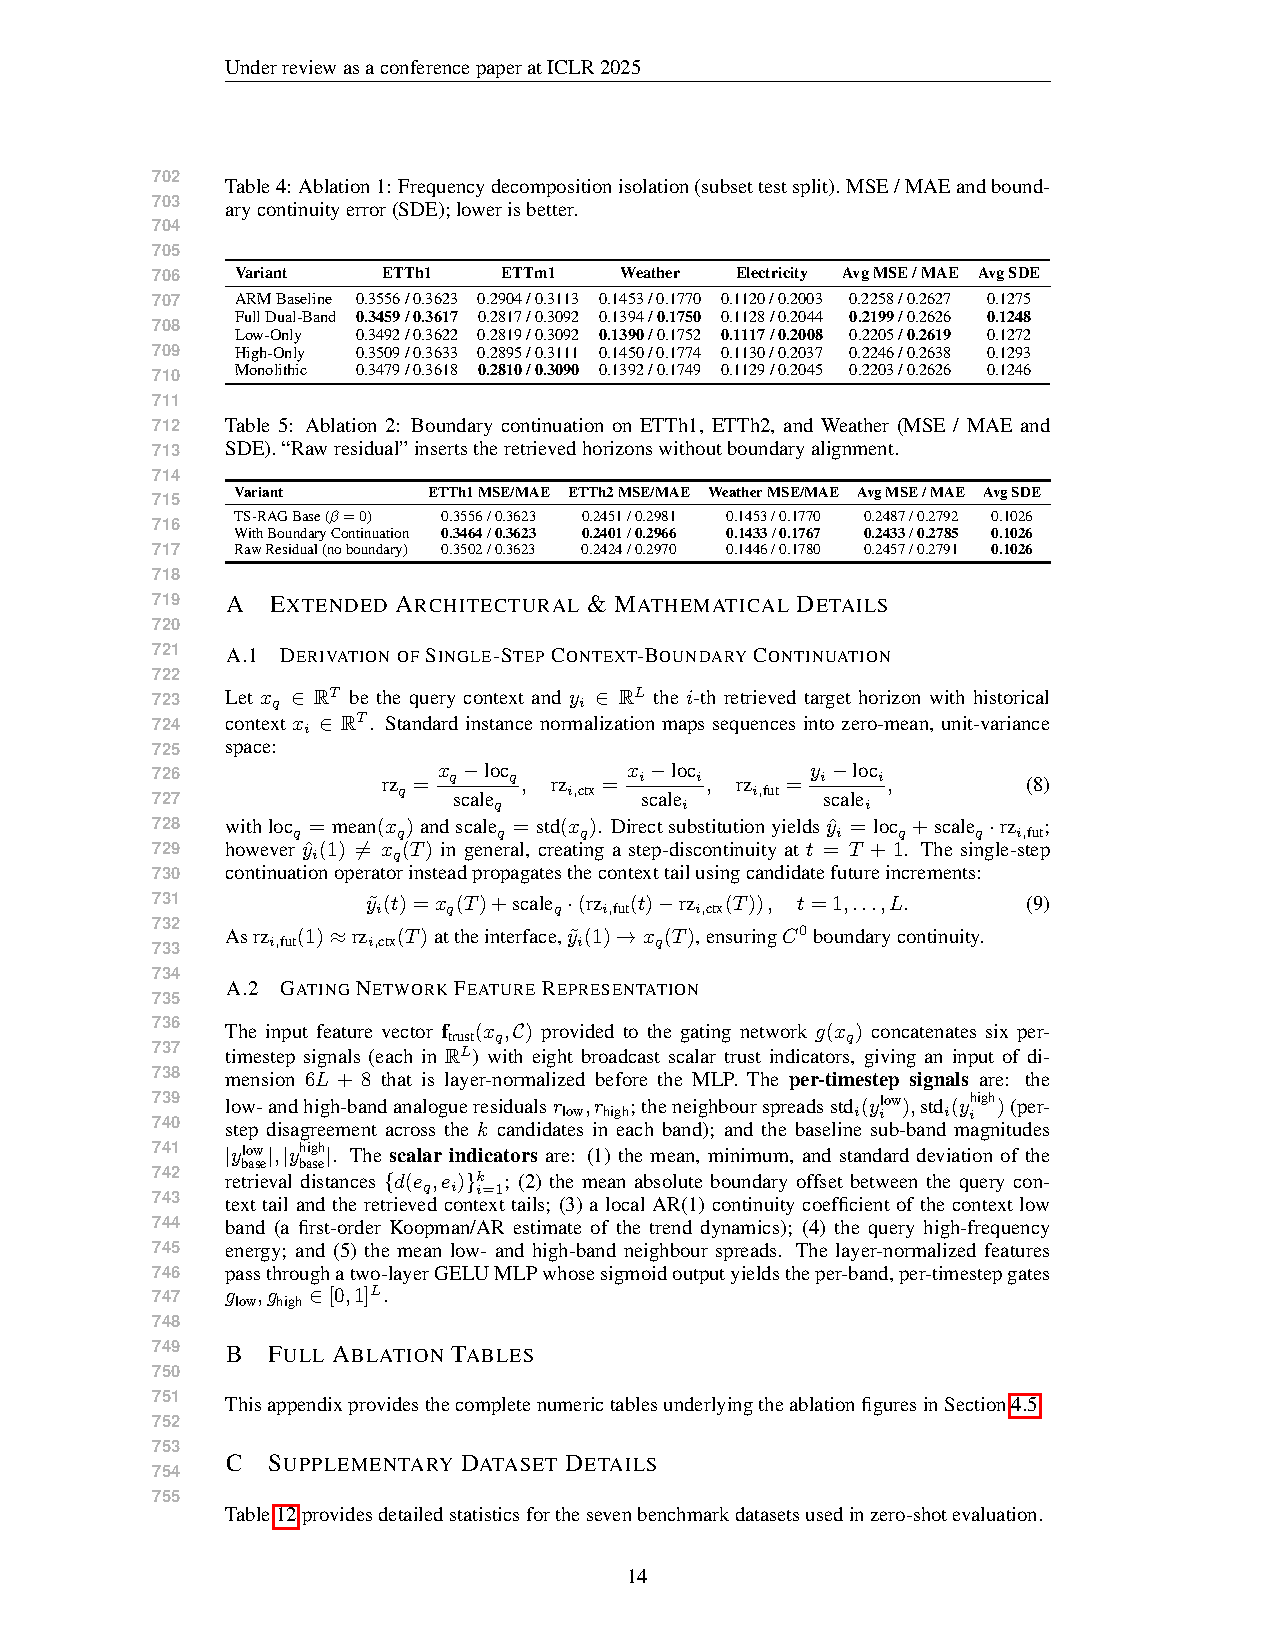
\includegraphics[width=\linewidth]{sections/dynaspec_qual/ts_rag14.pdf}
\end{figure}

\begin{figure}[t!]
    \centering
    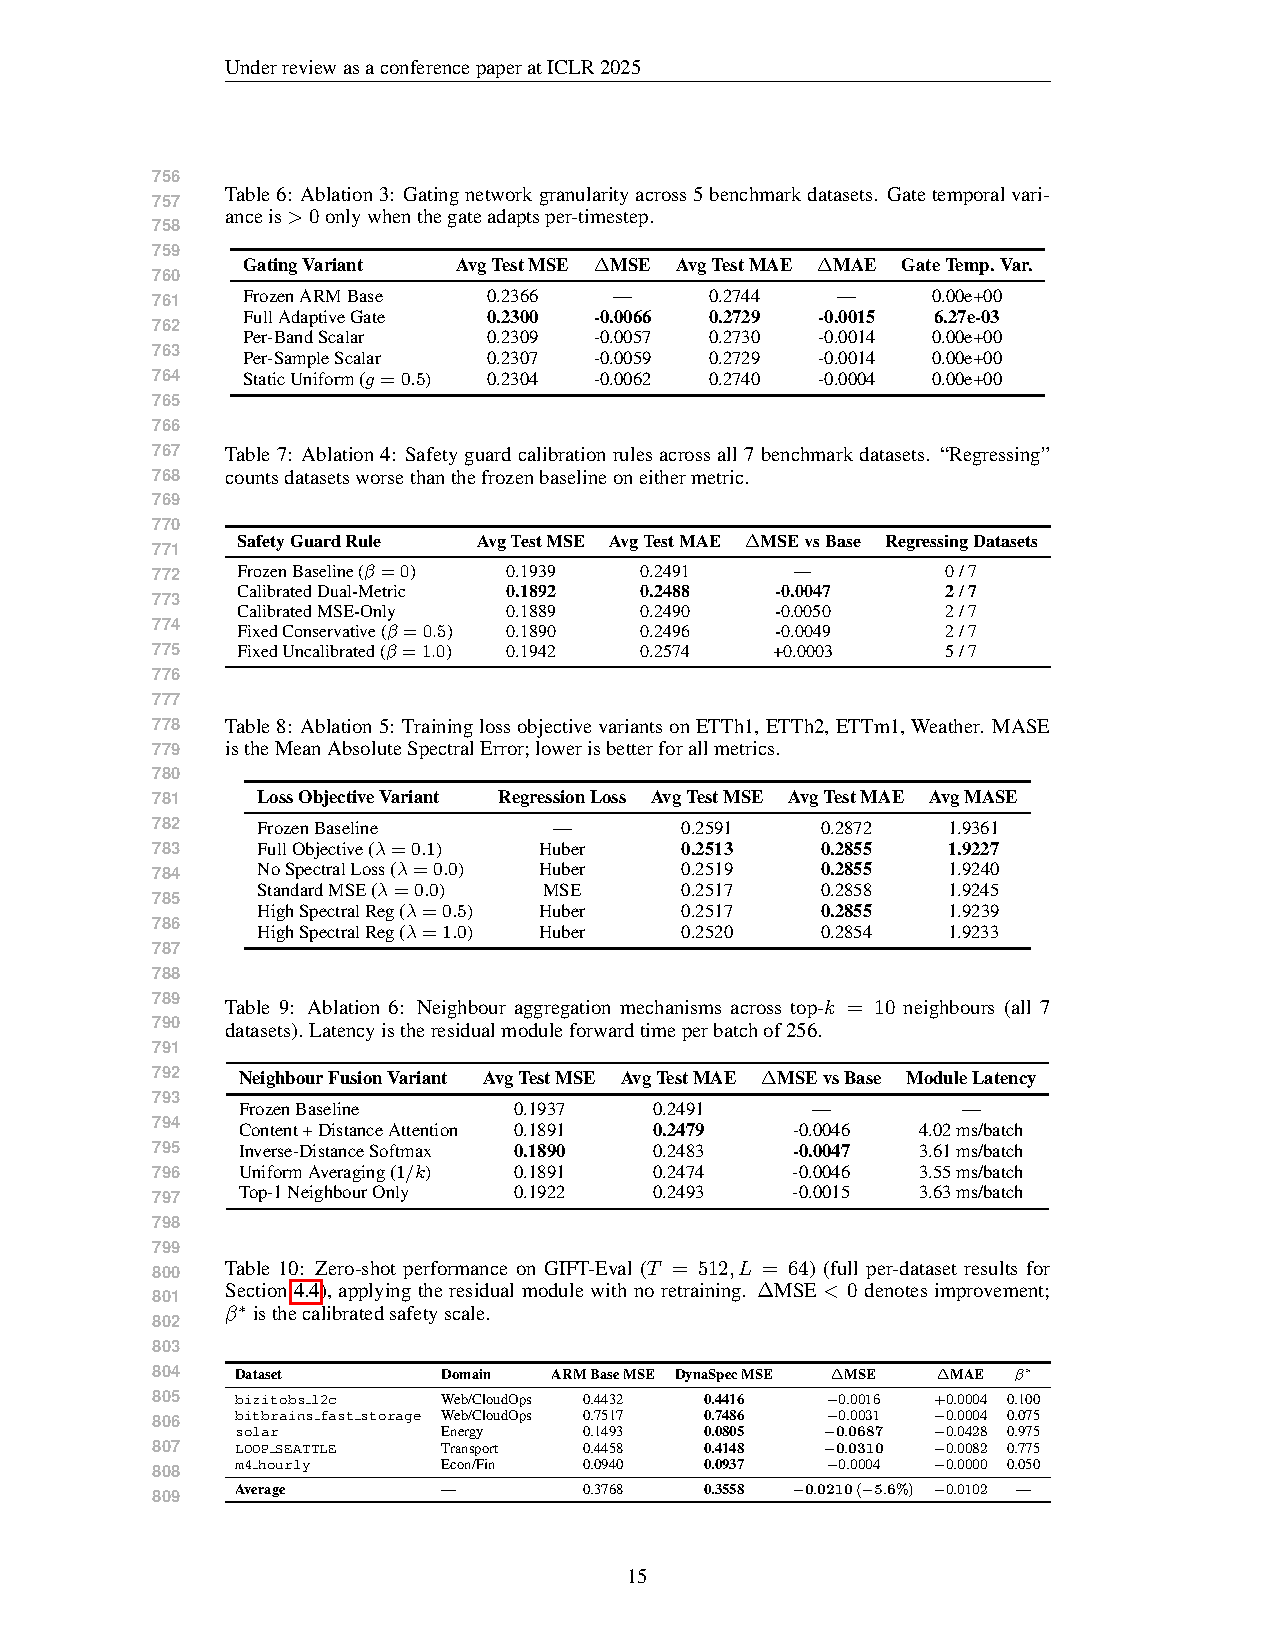
\includegraphics[width=\linewidth]{sections/dynaspec_qual/ts_rag15.pdf}
\end{figure}

\begin{figure}[t!]
    \centering
    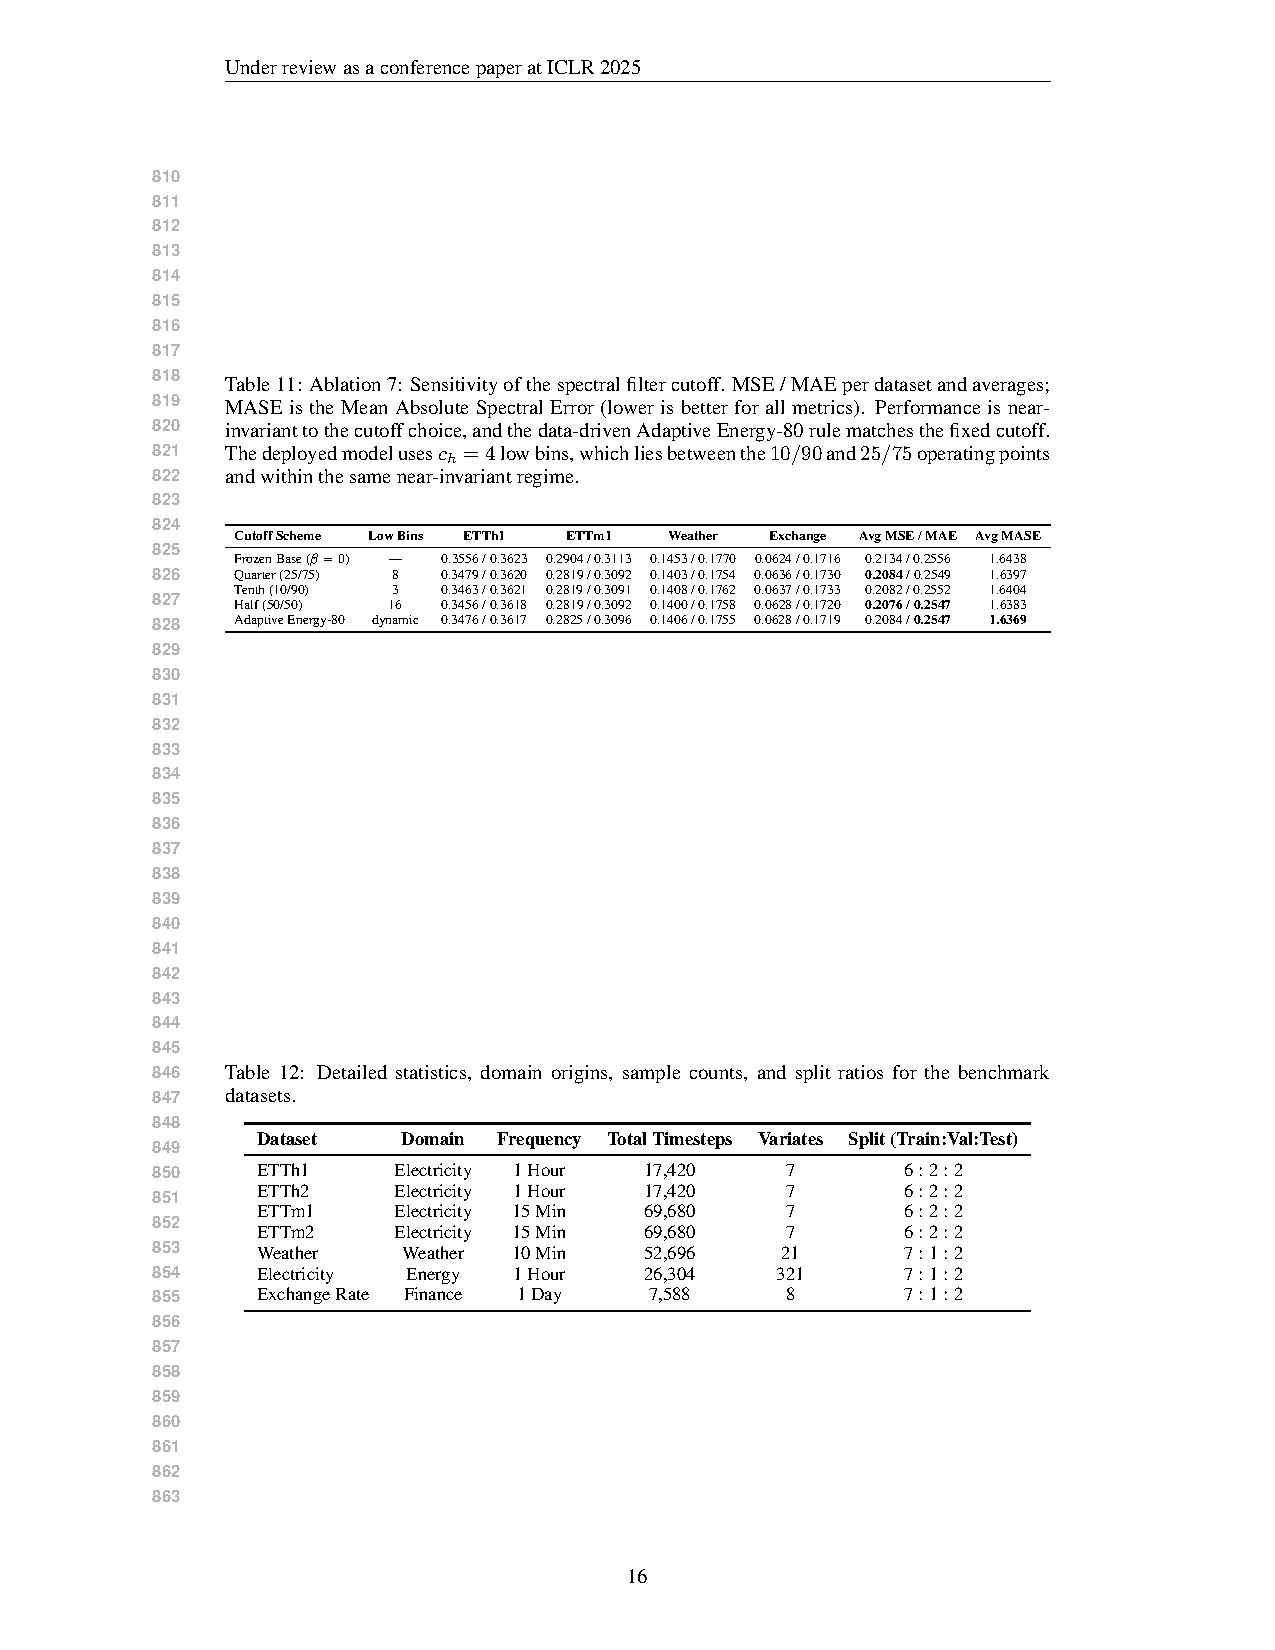
\includegraphics[width=\linewidth]{sections/dynaspec_qual/ts_rag16.pdf}
\end{figure}